% sage_latex_guidelines.tex V1.20, 14 January 2017
\documentclass[Afour,sageh,times]{sagej}

\usepackage{moreverb,url}
\usepackage[colorlinks,bookmarksopen,bookmarksnumbered,citecolor=red,urlcolor=red]{hyperref}
\usepackage{subfigure}
\usepackage{graphics} % for pdf, bitmapped graphics files
\usepackage{epsfig} % for postscript graphics files
\usepackage{mathptmx} % assumes new font selection scheme installed
\usepackage{times} % assumes new font selection scheme installed
\usepackage{amsmath} % assumes amsmath package installed
\usepackage{amssymb}  % assumes amsmath package installed
\usepackage{mathtools}
\usepackage{bm}
\usepackage{mathrsfs}
\usepackage{xcolor}
\usepackage{threeparttable}
\usepackage{multirow}
\usepackage{bigdelim}
\usepackage{algorithm}
\usepackage{algorithmicx}
\usepackage{algpseudocode}
\usepackage{graphicx}
\usepackage{comment}
\usepackage{galois}
\usepackage{array}

\newcommand\BibTeX{{\rmfamily B\kern-.05em \textsc{i\kern-.025em b}\kern-.08em
T\kern-.1667em\lower.7ex\hbox{E}\kern-.125emX}}

\def\volumeyear{-}

\setcounter{secnumdepth}{3}
\begin{document}

\runninghead{Tong Yang \textit{et al.} Smooth Non-repetitive Manipulator Coverage with Minimal Discontinuities}

\title{Smooth Non-repetitive Manipulator Coverage with Minimal Discontinuities}

\author{Tong Yang\affilnum{1}, Jaime Valls Miro\affilnum{2}, Yue Wang\affilnum{1} and Rong Xiong\affilnum{1}}

\affiliation{\affilnum{1} State Key Laboratory of Industrial Control and Technology, Zhejiang University, P.R.China\\
\affilnum{2} Robotics Institute (UTS:RI), University of Technology Sydney, Sydney, Australia}

\corrauth{Yue Wang, wangyue@iipc.zju.edu.cn}%, Yuquan Campus, Zheda Road 38, Xihu District, Hangzhou, China}


\begin{abstract}
%<TONG> abstract WAY too long. I tried to summarise further. Pls make sure what is left is correct.
%<TONG> we don't cite RSS20!!!! I will add a place for the citation in Section 1, see that you agree on how is referenced
A theoretically complete solution to the Smooth Non-repetitive Coverage Path Planning (SNCPP) problem of any arbitrarily shaped object with a non-redundant manipulator is proposed.  
SNCPP is a crucial task carried out by manipulators in industrial applications. Nonlinear manipulator kinematics and the imposition of task-specified constraints dictate that applying conventional Coverage Path Planning (CPP) solutions on the target surface invariably result in truncated end-effector motions. On the other hand, coverage paths designed directly in joint-space cannot ensure reoccurrences will not arise. 
%If considering the usage of non-redundant manipulator where the kinematic constraints are the severest, the problem becomes its most difficult form. 
Previous works have modelled the Non-repetitive Coverage Path Planning (NCPP) for non-redundant manipulators problem as the non-overlapping painting of a topological graph, constructed from valid (non-singular) simply-connected joint-space continuos configurations (each representing a single colour). %However, regardless of all singular configurations, the family of valid non-singular configurations form disjoint sets which individually is injective to the target surface under kinematic mapping. 
%Moreover, the surface to be manipulated is of simple shape and the task constraint is only the manipulability, which empirically ensure the simply-connected topology of cells in the graph. 
It has been proven that the family of simply-connected valid configurations form disjoint sets which are indvidually injective to the target surface via the kinematic mapping, and
%Under such assumptions, 
as such % <TONG> not sure this cause-effect link (injectiveness property leding to optimal solution) is true. Do you think this can be stated as this? 
all optimal solutions of the NCPP problem can be solved finitely. 
However, two key aspects have been omitted in these works. Firstly, singular configurations have been purposedly disregarded, hence invariably introducing end effector lift-offs at such poses bridging the continuous sets. 
Considering singular configurations violates the injectivity in the kinematic  mapping - hence the definition of a single colour per configuration. This work however proves that by carefully chosing permissible paths considering the rank-deficient manipulability measure, valid singularities can be leveraged to further reduce the number of necessary end-effector discontinuities.
%, hence reducing  and the manipulator EE need not suspend on the surface. 
%Considering singular configurations violates the injectivity in the kinematic  mapping - hence the definition of a single colour per configuration - a novel generalised modelling is proposed in this work. 
The scheme assumes generic represention of surfaces as discrete meshes, symbolising a null probability to locate the point corresponding to a singular IK solution, and constructs a practical method to smoothly traverse a singularity without explicitly calculating it. 
%to such a larger scope.
%Another one is that, given more sophisticated objects and more complex task constraints, the cells in the graph may be multiply-connected, whose finite solvablity has not been settled. 
Secondly, for sophisticated objects and more complex task constraints, the cells making up the graph may easily become multiply-connected. The proposed work further proves the finite solvablity for the generalised case, no matter what the resulting topological shapes from the constraints imposed on the cells may be, and a multi-stage iterative solver is designed to find all such optimal solutions. % <TONG> this is not true, we do in RSS20!
%Compared with previous works, the first contribution of this paper is to propose the necessary and sufficient condition for all kinds of task constraints that enables us to transform the SNCPP problem into a topological graph solving problem. 
%The second contribution of this paper is to generalize the scope from considering only regular configurations to also valid singularities given by the usage of rank-deficient manipulability measure, and coming up with the solution of leveraging singularities to further avoid end-effector lift-offs compared with abandoning all singularities. 
%And a mechanism to avoid end-effector suspension on the mesh is also proposed in considering both the analytic surface case and discrete representation case. 
%The third main contribution of this paper is a classification of cells through their genus, or the number of ``holes" which appear increasingly as configurations are further constrained with the introduction of additional metrics for the task at hand, e.g. manipulability thresholds, clearance from obstacles, end-effector orientations, tooling force/torque magnitudes, etc, and show that no matter what the resulting topological shapes from such quality cell constraints may be, the graph is finitely solvable, and a multi-stage iterative solver is designed to find all such optimal solutions. 
Extensive simulated and realistic experiments are carried out for examination of the proposed algorithm. 
\end{abstract}

\keywords{Optimal Cellular Decomposition, Non-repetitive Coverage Task, Non-redundant Manipulator}

\maketitle

\section{Introduction}
Full coverage of the surface of a given object with non-redundant manipulators is embodied in tasks such as automatic polishing~\cite{Tian2016Polishing}, deburring~\cite{Xie2016Grinding}, painting~\cite{Li2011Painting} or surface inspection~\cite{Molina2017Defects}, where the need for smooth non-repetitive coverage path planning (SNCPP) is paramount to avoid over revisiting. 

The kinematic relationship of a typical manipulator makes mapping between work- and joint-space non-bijective~\cite{lavalle2006planning}, which in effect drives coverage paths to be traditionally carried out in the former to ensure no revisiting of points in the surface~\cite{Oriolo2005Motion}. 
However, in further pursuing motions where the manipulator may minimise the number of reconfigurations is obliged to undertake to follow a desirable continuous end-effector (EE) path, a global optimal cellular decomposition problem in joint-space has been 
proposed to incur joint-space partitions with minimum sets~\cite{Yang2020Cellular}. 
This is illustrated in the example shown by Fig.~\ref{fig:TMech}: the external surface of a wok-like object is inspected by a non-redundant manipulator. 
Points on the surface can be reached by a variety of robot configurations. 
The three solid colour cells shown in Fig.~\ref{fig:TMech_config_cells} illustrate poses of disjoint sets reachable as a continuous set by a given configuration, visually seen by the different colours. 
These cells become the elements on a topological graph Fig.~\ref{fig:TMech_topo_graph}, where each possible colour of a cell is recorded. 
A cellular decomposition splits and merges the cells to transform the process into that of painting all points in the graph with one of the possible colours, driven by attaining a minimum set which equates to least number of EE lift-offs. 
One such optimal solution with 2 lift-offs is illustrated in Fig.~\ref{fig:TMech_solution}, 
whereby any arbitrary continuous coverage path within a colour surface area will result in maxium joint continuity of the global path. 
The addition of obstacles and the relative pose of robot and object further condition the final solution. 
\begin{color}{blue}
%The difficulty of the focused problem can be revealed through comparison to some widly-developed complex problems. Following the same vein of problem modelling in~\cite{Yang2020Cellular}, the repetitive CPP problem can be modelled as the \textit{Minimum Set Cover} problem which is a NP-complete problem in the computer field. 
%The repetitive CPP problem is an easy version of the SNCPP problem since the path that has been visited does not effect the subsequent CPP task.  
%As for the non-revisiting constraint, it is commonly investigated in the Traveling Salesman Problem which is though defined in discrete node graph but is still NP-complete. 
%Affinities to graph theory are legit. 
%Note however that the contact point, which can be safely regarded as a particle, 
%is significantly smaller than the scale of the cellular decomposition drawn up for this problem. 
%In seeking maximal joint-space continuity of the coverage path travelled by a particle as modelled by the SNCPP problem, 
%infinitesimal elements must be considered in its most abstract form, and the existance of infinitely narrow passages also 
%makes a significant difference in the resulting path solutions. 
%Hence, it is not possible to revert back to classical graph theory since no any area on the surface can be seen as an inseparable whole to form the ``vertices", and the set of ``edges" is actualy the exact solution the SNCPP problem is seeking to solve for. 
However, it is noticable that in order to model the original NCPP problem to an abstract form, strong assumptions were made to the NCPP problem~\cite{Yang2020Cellular}, which inspires two directions for further development. 
\end{color}

\begin{figure}[t]
\centering
\subfigure[]{
	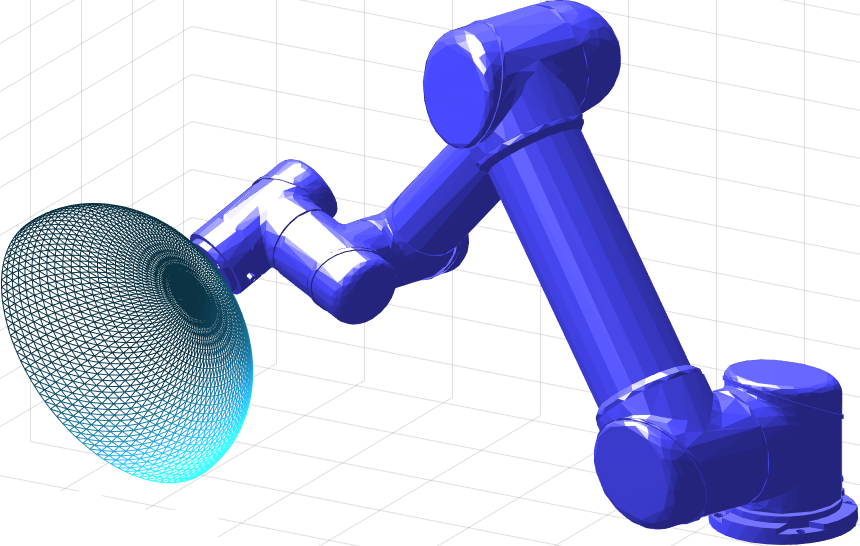
\includegraphics[width = 0.1\textwidth]{figures/TMech_simply_connected_example/design_demo_2}
	\label{fig:TMech_model}}
\subfigure[]{
	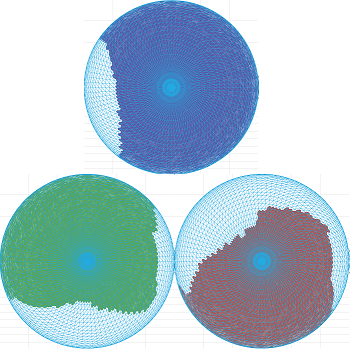
\includegraphics[width = 0.1\textwidth]{figures/TMech_simply_connected_example/design_comb}
	\label{fig:TMech_config_cells}}
\subfigure[]{
	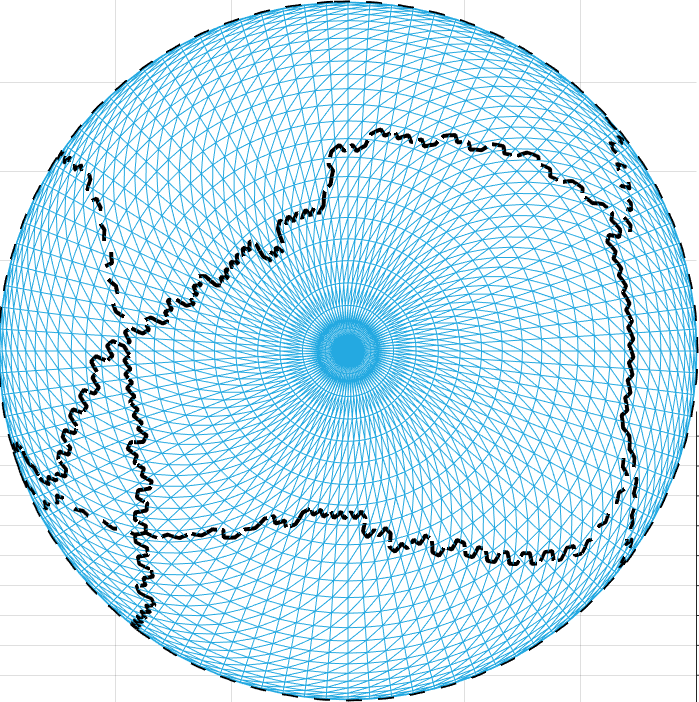
\includegraphics[width = 0.1\textwidth]{figures/TMech_simply_connected_example/design_init_graph}
	\label{fig:TMech_topo_graph}}
\subfigure[]{
	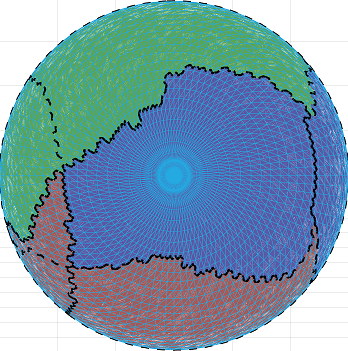
\includegraphics[width = 0.1\textwidth]{figures/TMech_simply_connected_example/design_result_graph}
	\label{fig:TMech_solution}}
\caption{Example of simply-connected cell coverage. (a) Hemispherical object placed in the workspace. 
(b) Simply-connected cells of three valid robot configurations, chosen by the optimal solution shown in (d). 
(c) Topological graph. (d) One optimal solution requiring 2 lift-offs. 
}\label{fig:TMech}
\end{figure}



\begin{figure}[t]
\centering
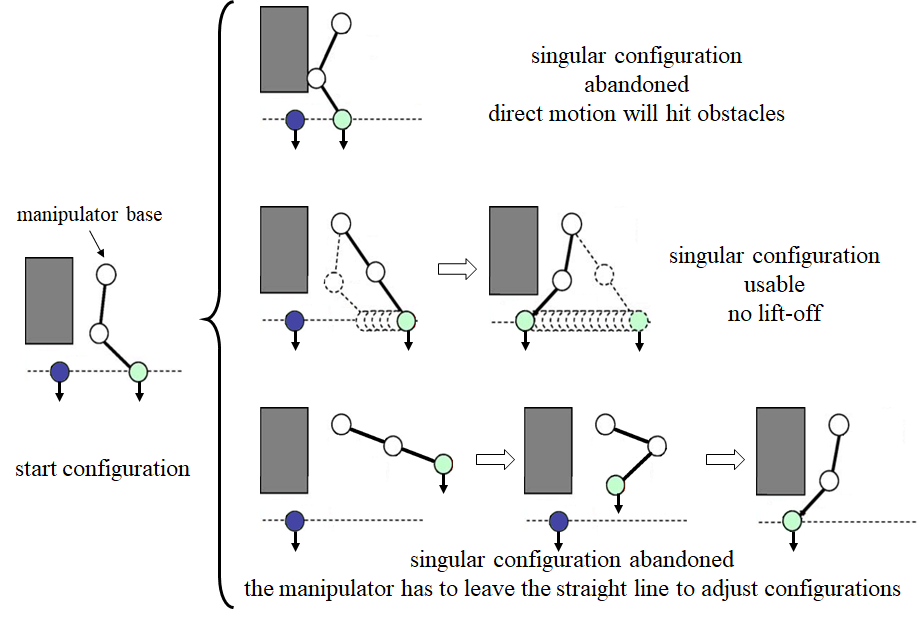
\includegraphics[width = 0.44\textwidth]{figures/other_figures/2dof_demo}
\caption{
Illustration of using a valid singular configuration to avoid one EE lift-off. To simplify the description the example is taken as a repetitive CPP task. With the last joint keeping the EE perpendicular to the dashed line, the 3DoF RRR manipulator is non-redundant. Starting from an elbow-left pose, the obstacle (gray block) obstructs the smooth EE motion towards the goal pose (the upper case). 
It is apparent that there is a valid singular configuration when the EE moves to the right most, an ``elbow-middle" configuration which smoothly connects the elbow-left poses and elbow-right poses, which reduces the number of lift-off to zero (the middle case). 
If we directly disregard all singular configurations, then one EE lift-off is required (the lower case). 
}\label{fig_2dof_demo}
\end{figure}

\begin{figure}[t]
\centering
\subfigure[]{ 
	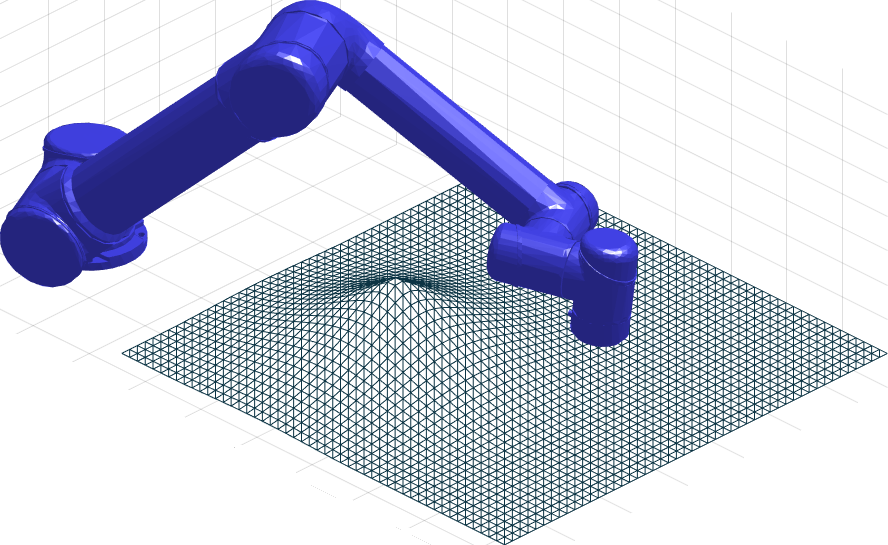
\includegraphics[width = 0.1\textwidth]{figures/RSS_related_figures/hill_exp/0_06/new/demo}
	\label{fig:hill_model}}
\subfigure[]{	
	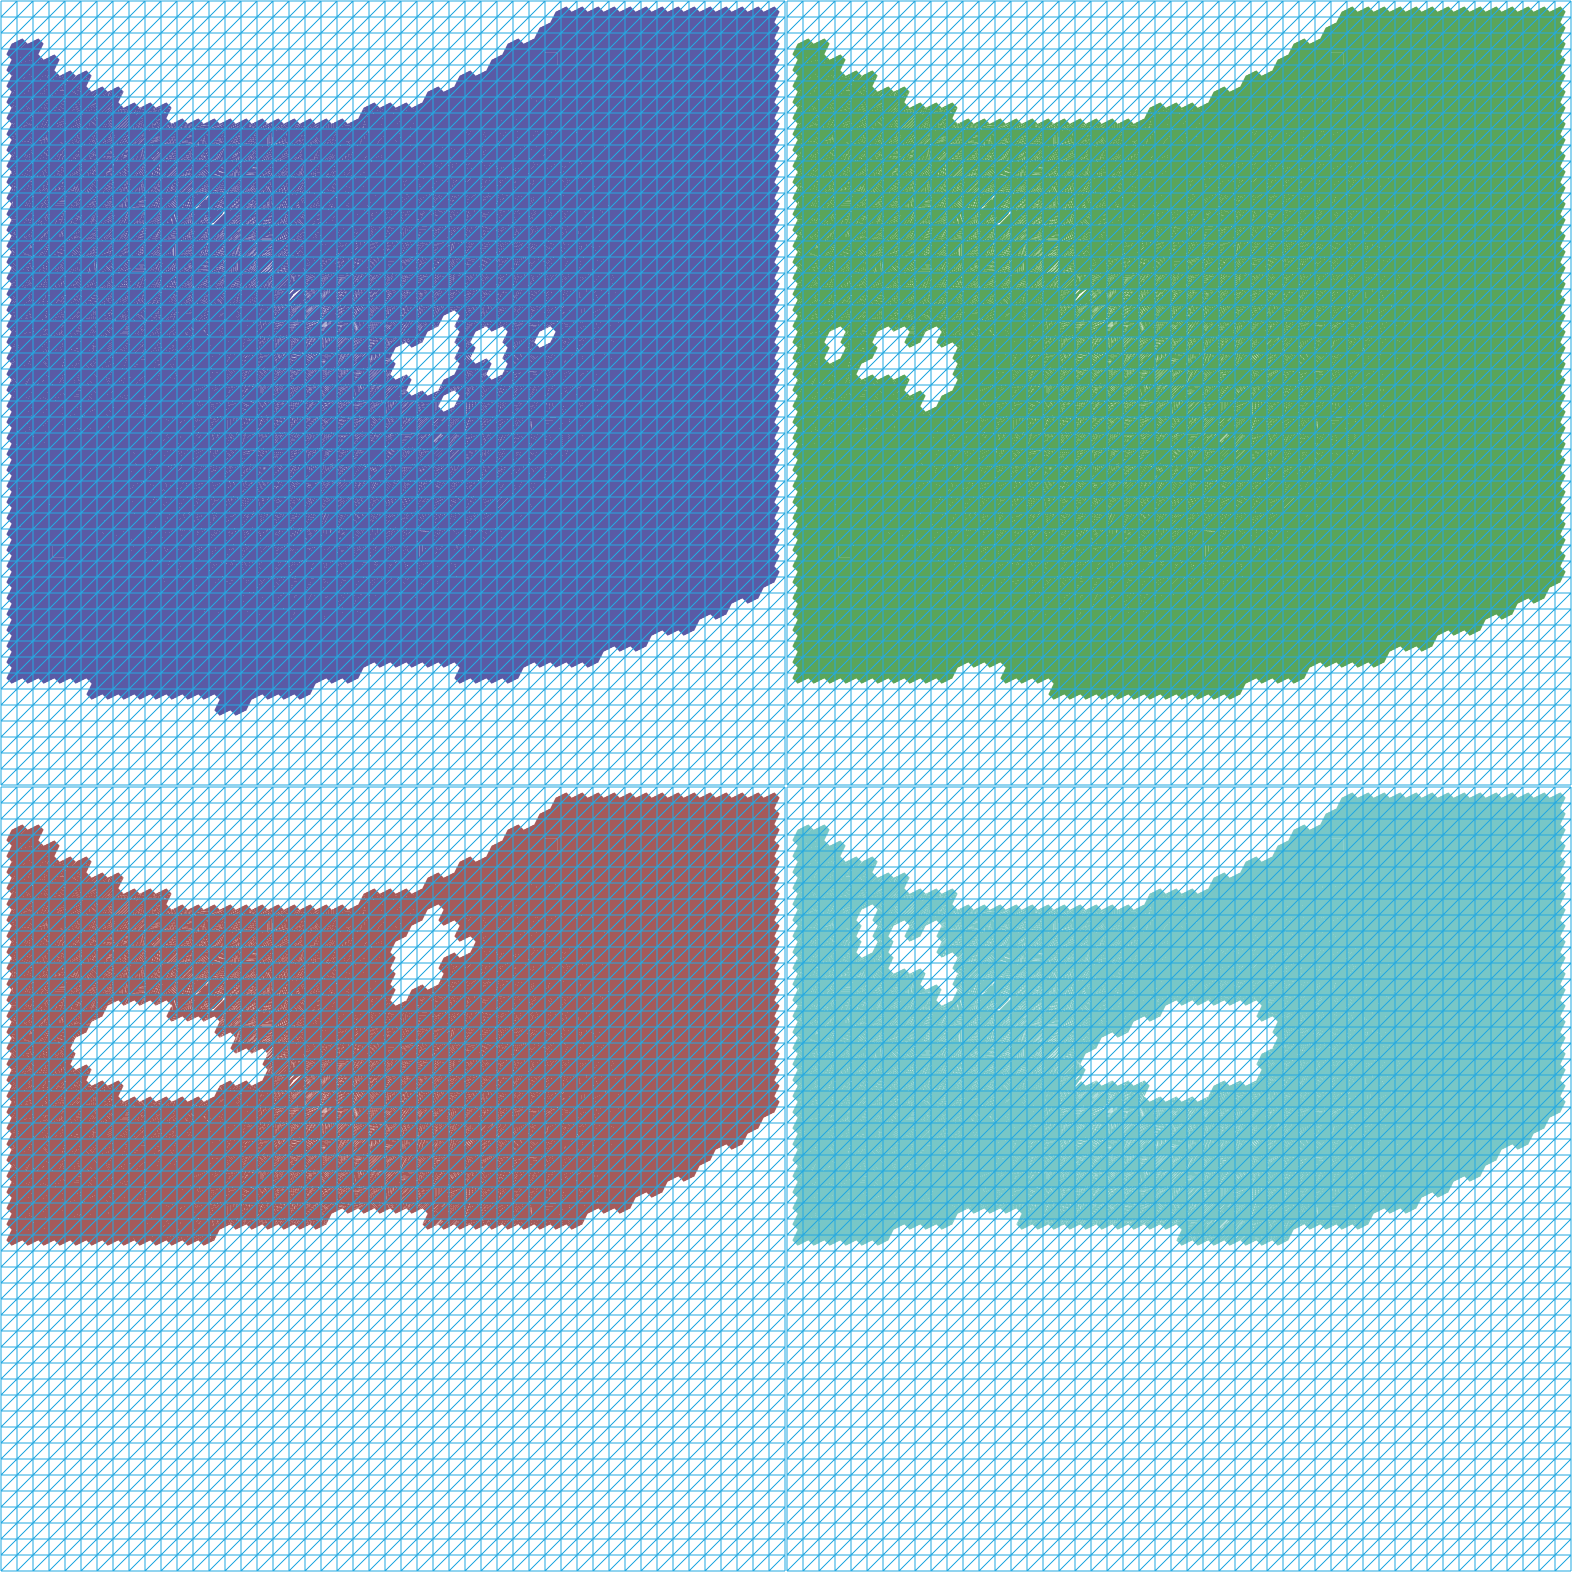
\includegraphics[width = 0.1\textwidth]{figures/RSS_related_figures/hill_exp/0_06/new/color_comb}
	\label{fig:hill_config_cells}}
	\subfigure[]{	
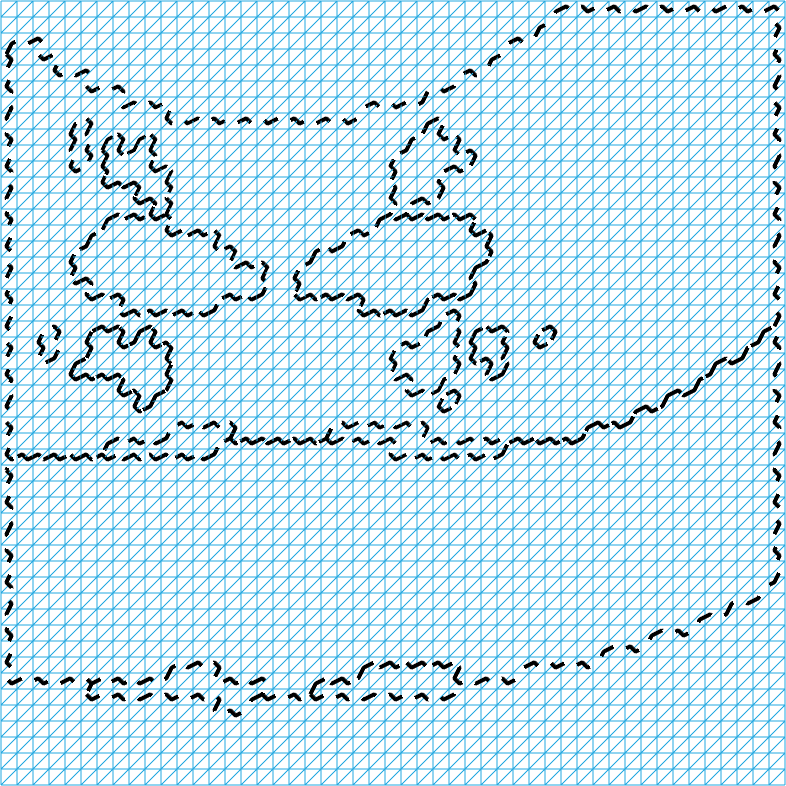
\includegraphics[width = 0.1\textwidth]{figures/RSS_related_figures/hill_exp/0_06/new/init_graph}
	\label{fig:hill_topo_graph}}
\subfigure[]{	
	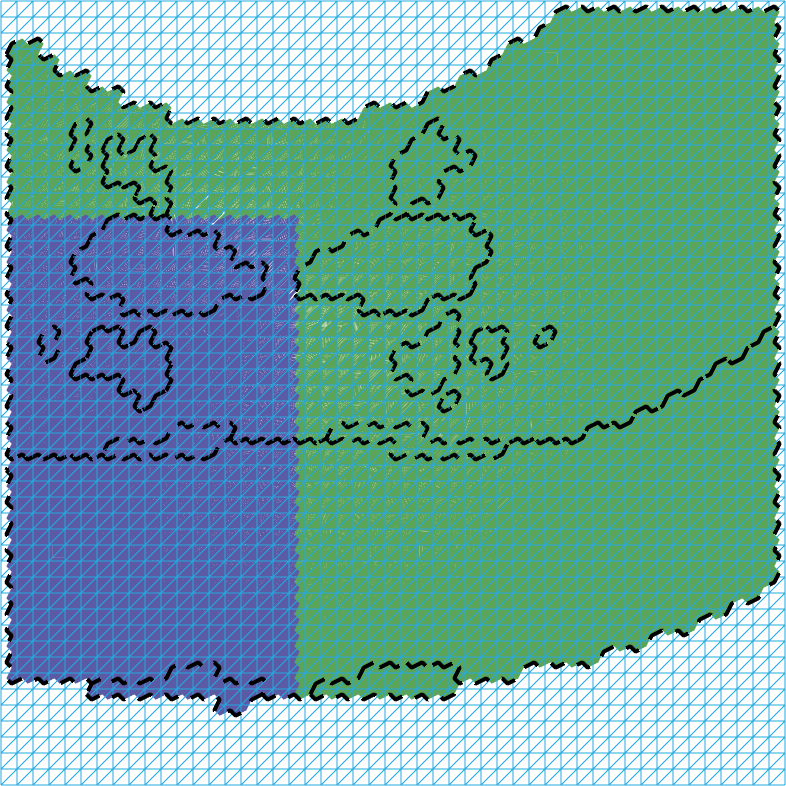
\includegraphics[width = 0.1\textwidth]{figures/RSS_related_figures/hill_exp/0_06/new/result_graph}
	\label{fig:hill_solution}}
\caption{Example of multiply-connected cell coverage. (a) Irregular ``hilly'' object placed in the workspace. 
(b) Multiply-connected cells of four valid robot configurations, chosen by the optimal solution shown in (d). 
(c) Topological graph. (d) One optimal solution requiring 1 lift-off.}
\label{fig:hill_multiply_conn}
\end{figure}



\begin{color}{blue}
First, all singular configurations are not considered in the coverage task because they lack the capability to dispense with the pertubation in some directions on the EE. This is indeed valid but is too conservative: if the pertubation in some dimensions can be safely disregarded, then singular configurations may also be valid. One most illustrative example can be seen when using a planar 3DoF manipulator covering the line segment, as shown in Fig.\ref{fig_2dof_demo}, where with the usage of an ``elbow-middle'' configuration, the elbow-left configuration is essentially joint-space continuous to the elbow-right configuration that has the same EE pose. 
Another example is that, such as in Fig.\ref{fig:TMech} and Fig.\ref{fig:hill_multiply_conn}, the EE link does not have twist offset with respect to the last link of the manipulator, thus there is no pertubation of EE torque that the manipulator need to deal with. 

For clarity, when the manipulator covers a point on the surface using a valid ``singular configuration", we refer to the point that the EE covers as a ``singular point" in contrast to ``regular point" on the surface. 
When considering the valid singular configurations in the scope of the problem, the geometric coverage path cannot be arbitrarily designed with in a result cell, because (1) At regular point, the kinematic mapping between a continuous set of valid configurations and the surface is no longer bijective. (2) At singular point, there are infinite many IK solutions which cannot be fully pre-calculated, and the manipulator EE is unable to move omnidirectionally on the surface~\cite{Egeland1991Manipulator}. And a problem in realistic environment destroys all possible generalizations from existing solution: (3) The surface is always represented in discretized form (triangular mesh, point cloud, etc.), on which there is zero probability to find a singular point. 

To understand (1), see the planar example in Fig.\ref{fig_2dof_demo}, an elbow-left pose and an elbow-right pose are continuous only if the ``elbow-middle" pose stays with them, as per they will be assigned with the same colour. Then, a coverable colour of a point does not uniquely correspond to one valid IK solution, thus a coverage path within the coverable area of a colour does not correspond to a unique joint-space path solution. 
Moreover, the worst thing is that the division of the area may lose joint-space continuity. 
If we do task-space divisions in the planar case shown in Fig.\ref{fig_2dof_demo}, which is taking an intermediate segment in the dashed line, such as one without the right-most point, then the elbow-left and elbow-right IK solutions to cover its points are essentially not joint-space continuous even if they have been given the same colour. 

To appreciate (2), when a non-redundant, say 5DoF, manipulator becomes singular, it essentially performs like a 4DoF one, where the missing one DoF gives rise to the \textit{null motion}, during which the manipulator is adjusting pose but the EE remains static. 
This calls for realistic demand to the joint-space coverage path with smooth motion of the EE on surface. More precisely, the EE cannot stop at a point for a while, for the force applied to the surface does extra work at a single contact point if the EE suspends, leading to possible damage to the surface. 

As for (3), the non-redundancy of the manipulator means that given an EE pose, there are only finite number of solutions, mainly due to the nonlinearity of the inverse trigonometric functions used for solving revolute joints' motion. The overall system of equations is a determinate system. When a non-redundant manipulator is enforced to be singular, the system is overdeterminated, i.e., has no solution unless in some exceptional case. Thus the singular points on the given surface form only zero-area region, which has zero probability to be sampled when the surface is represented in discrete form. 


\end{color}


%\begin{color}{red}
%When a non-redundant manipulator becomes singular, the EE is unable to move along its \textit{degenerate directions}~\cite{Egeland1991Manipulator}, thus is not omni-directional, which calls for extra consideration in the subsequent coverage path planning (CPP) process. 
%A realistic demand is the smoothness of the joint-space coverage path without sharp turns and suspendings on surface, i.e., the EE cannot stop at a point for a while, because the force applied to the surface does extra work at the contact point if the EE suspends for a while, leading to possible damage to the surface. 
%In the traditional CPP area, the smoothness of the geometric coverage path is established through locally modifying the shape of the geometric coverage path, such as locally replacing sharp corners with arcs, and the global innovation from the back-and-forth motion~\cite{Choset1998Coverage} to the spiral-like path~\cite{Hassan2018A}. 
%However, recall that the CPP solution is carried out in the work space, pure coverage path planner cannot obay the constraint given by manipulators when it is singular. 

%We would say that encounting valid singular configurations is not an exceptional case and is inevitable, since using non-full rank measure as a criterion for judging the valid configurations is frequently used, and we need not (and are impossible for $<6$ DoF manipulator to) consider the robustness of the EE motion in all dimensions (a $SE(3)$ space). 
%For example, in Fig.\ref{fig:TMech} and Fig.\ref{fig:hill_multiply_conn}, the EE link does not have twist offset with respect to the last link of the manipulator, thus there is no pertubation of EE torque that the manipulator need to deal with. 

%The difficulty of broadening the horizon of the SNCPP problem to envolve valid singular configurations is that, with a degree of redundancy, there are infinite many inverse kinematic solutions of a same EE pose, which leads to failure of specifying each configuration a \textit{colour}~\cite{Yang2020Cellular}. 
%Moreover, the discrete representation of the surface further compounds the problem, since we also have zero possibility to locate the points where the manipulator is singular, which is referred to as \textit{singular point} in this paper. 
%The key observation of dealing with the singularities is that the singular points form zero area set, thus whether the coverage path explicitly passes them or overlooks them makes no difference to the performance of the coverage task. And in realistic application the physical contact region between the EE and the surface must be a small region but not a particle point which can compensate the neglect of covering such points to some extent. 
%In other words, the singular configurations only do good to the task. Only what we need to do is considering leveraging singular configurations. 
%\end{color}

\begin{color}{blue}
Another observation to the existing solution of the NCPP task is the existence of multiply-connected cells in the topological graph. 
%When the object has simple surface shape and the constraint in the task is only the manipulability which removes all singular configurations, the generated topological graph often contains only simply-connected cells. 
%The connectivity of a 2D region is a basic concept in algebraic topology. A region is simply-connected means that all closed paths in the region can continuously shrink to a point, so called \textit{the homotopy class of paths is trivial}, while in multiply-connected region there exist non-homotopic closed paths. In previous works~\cite{Yang2020Cellular}, the finite solvability and the solutions are only applicable in graphs consisting of totally simply-connected cells. 
%Although empirically the case of graphs with simply-connected topology can cover large proportion of realistic applications, given complex shape of the surface to be covered and more complicated task-specific constraints, the graph may contain multiply-connected cells whose finite solvability and optimal solutions are still unsettled issues. 
\end{color}
%we further notice two aspects that generalise the scope of the applications. 
%One progress made in this paper is the observation that some singular configurations are still valid under the usage of rank-deficient manipulability measure, such as the \textit{tranlational manipulability}~\cite{yoshikawa1990translational} which only considers the ability of tranlational motion of the EE. 
%\begin{color}{blue}
%Another advance in this paper is that we remove the assumption of simply-connected topology of cells in the topological graphs. 
%\end{color}
A critical assumption to adapt the solver proposed in previous work is that the constituent surface points necessarily adopt simply-connected space topologies. 
This is reasonable for simple shapes and sparse obstacle environments, but becomes unrealistic as objects grow in complexity, 
or with the imposition of increasing motion constraints, generically deriving in multiply-connected cells. An illustrative example is given in Fig.~\ref{fig:hill_multiply_conn} where a manipulator moving over a ``hilly'' terrain generates reachable areas in the mesh which contains non simply-connected cells. 
\begin{color}{blue}
The hole appears because whatever kinds of configurations the manipulator is using, when the wrist is about to hit the hill, it has to stop and changes the configurations. And in this problem it is intuitive to see that changing between shoulder-left poses and shoulder-right poses for one time will be enough for avoiding collision with the hill, thus $1$ lift-off is the optimal solution, and the geometric specification of coverage area to different poses has large flexibility, as shown in Fig.\ref{fig:hill_solution}. 
\end{color}
The problem is further compounded when additional or more restrictive constraints are imposed, 
 as will be seen later in the results when the degree of manipulability is also considered and more ``cavities'' appear in the configuration cells and generated topological graphs.

Since the shape of cells can be classified through their genus, i.e., the number of ``holes" within the cell, in this work a 
theoretically complete solution is given by solving for cells with all possible genus. The key observation of the proposed algorithm is that whatever genus the cell is, the number of lift-off to cover it is always zero. 
A direct reflection from this is thus to reduce the genus of the cell gradually by cell divisions to eventually make it equivalent to a simply-connected cell which has been proven finitely solvable. 
This however is non-trivial: the place to put a cutting path to transform 
a genus-one cell into a simply-connected cell directly effects the order of edges on the boundary of the sub-cells, leading to different structures. 
\begin{color}{blue}
And we are interested in discovering all optimal topological solutions, because from one of the proposed solutions the practitioners can freely make any continuous modification to the shape of the cutting paths to form any geometric cellular decompositions suitable for their tasks. 
\end{color}
Existing algorithms in the literature are not able to provide a systematic cell decomposition solution to accomplish a guaranteed 
transformation from an initial graph containing large genus cells into simply connected topologies. 

\begin{color}{blue}
This work aims to fill in the above mentioned gaps towards a systematic solution of the SNCPP task using non-redundant manipulators. The three novel contributions of this paper can be summarized as:
\begin{enumerate}
\item We closely examine the geometrical distribution of the valid configurations containing valid singularities, enlarge the applicable horizon of modelling the SNCPP problem as a painting problem of graphs, and prove the existence of the smooth non-repetitive coverage path planning solution. 
\item We particularly discuss the applicability of a topological graph-based algorithm running on discretely represented surfaces leveraging valid singular configurations without explicitly finding the singular points. 
\item Finally, arbitrary genus cells are iteratively transformed into lower-genus cells under equivalent topological divisions, up to several simply-connected cells whose finite solvability has been proven. Following by existing enumerative solver~\cite{Yang2020Cellular} of a whole topologial graph, all graphs are proven finite solvable and all optimal solutions can finally be collected. 
\end{enumerate}

%This is provided in this work through 
%the analysis of equivalent topological divisions. To that extent, the finiteness of all possible divisions is first proven for a genus-one cell as 
%building block. A multi-stage iterative solver can then be introduced to transform higher-genus cells into lower-genus cells. 
%\begin{color}{blue}
%Through enumerative solving all cells, all optimal solutions can finally be collected. 
%\end{color}



%The three novel contributions of this paper can be thus summarised as:
%\begin{enumerate}
%\item Providing the necessary and sufficient condition to be able to apply the surface modeling described by the proposed topological graph structure. 
%\item Proposing a detailed discussion to the optimal SNCPP task on analytically or discretely represented surface. 
%\item Proposing a systematic solution to be applicable for any genus-$n$ cell topology. 
%\end{enumerate}


The remainder of this paper~\footnote{A video illustrating the concepts hereby described can be found 
here:\url{https://youtu.be/TqFzqGGM06Y}} is organised as follows. 
Section~\ref{section_related_works} reviews existing literature. 
Section~\ref{section_problem_statement} states the problem and proposed the necessary and sufficient condition to apply the proposed algorithm, which are detailedly proved in Section~\ref{section_finiteness_of_cells}. 
Section~\ref{section_analytic} considers the lift-off avoidance through passing the singular configurations in analytic surface.
Section~\ref{section_discrete} presents the necessary and sufficient condition for the SNCPP problem to be solved on discretized surface data. 
Section~\ref{section_simply_connected} briefly restates the existing results in~\cite{Yang2020Cellular} to solve for 
simply-connected cells. 
Section~\ref{section_genus_one} goes into further details about the finiteness of solving elementary genus-one cells, whilst 
a multi-stage iterative strategy to solve for larger genus-$n$ cells is described in Section~\ref{section_large_genus}.
Experimental results from simulations are collected in Section~\ref{section_exp}, with final concluding remarks gathered in 
Section~\ref{section_conclusion}.
\end{color}

\begin{color}{blue}
\section{Related Works}\label{section_related_works}
\end{color}

This work combines the traditional coverage path planning algorithm with the manipulator kinematics. Besides, the manipulator motion at the singularity and the sampling strategy on the constrained manifold are also considered. Here we briefly introduce them separately.  
\subsection{Coverage Path Planning}
The classical solutions of the coverage path planning (CPP) problem consists of two parts: dividing the robot's workspace into simple, easily handled cells, so called the cellular decomposition, and then planning a geometric coverage path considering the kinematic of the robot within each cell. 
The cellular decomposition algorithms can be classified into two categories: exact cellular decomposition methods~\cite{lumelsky1990dynamic} and Morse-based cellular decomposition methods~\cite{choset2000exact}~\cite{Acar2002Morse}. 
Exact cellular decomposition methods divide the free space into trapezoidal or polygonal sub-regions. 
Morse-based cellular decomposition methods apply divisions of the free space based on the critical points of Morse functions to present more flexible shapes for cells over those extracted by exact cellular decomposition. A combination of Morse decomposition and Voronoi diagrams~\cite{Choset2000Sensor-based} has also been proposed, particularly fitting to cover vast open spaces and narrow areas simultaneously.
~\cite{Atkar2003Towards} optimised the coverage path through choosing optimal starting points.
~\cite{Huang2001Optimal} reduced movement cost by remaining on straight paths as long as possible thus minimising the number of turns.
~\cite{Jimenez2007Optimal} used a genetic algorithm to achieve optimal coverage.
~\cite{Oksanen2009Coverage} considered practical aspects of agricultural machines in agricultural field plots and used a greedy strategy for cellular decomposition.

As for the geometric coverage path designing, the most widly-used ones are the boustrophedon path and the spiral path, where the former is easily to be adapted in polygonal shaper cells, and the latter one is of high energy efficiency~\cite{Mei2004Energy} because of the avoidance of the sharp turns which calls for acceleration and deceleration of the robot.~\cite{Hassan2018A} proposed a deformable spiral coverage path planning (DSCPP) algorithm to fit the spiral path inside a minimum bouding rectangle (MBR) of the area to be covered, under the assumption that the path is not necessarily to be strictly within the boundary of area. 

The non-repetitivity in the classical CPP problem is trivial, as the cellular decomposition is directly carried out on the task-space (the surface), leading to all cells non-overlapped. However, it is worthwhile noting that despite the apparent similarities in planning with mobile platforms, the discontinuities and suspensions while executing the coverage task is inherent to the kinematics of manipulator mechanisms, and as such beyond the scope of bibliograpic works from the mobile robotics community. How to generate a task-space coverage path containing maximum joint-space continuity remains a open problem.
One method to evade this problem is to restrict the object to be so small and flat that does not require large motion of the manipulator. In this case, essentially there exists such a joint-space path that is able to track the non-repetitive task-space coverage path, as done in~\cite{Atkar2008Hierarchical} for uniform coverage in automative spray painting problem. 
Another method is to use redundant manipulator~\cite{Hess2012Null}, mobile manipulator~\cite{Atkar2003Towards}~\cite{Ren2017A} or multi-manipulators~\cite{Hassan2016Modeling} for more flexibility, and hopefully the desired path can be found in a higher dimensional joint-space. 
However, the problem is never positively resolved. 
%~\cite{Ren2017A} considered the base position optimization of a mobile painting manipulator, which is actually an optimization of redundant manipulator following a given coverage path, under the assumption that the manipulator executes the painting task after the mobile base moves to a given position and stops. 
For a generic coverage task, the problem is inevitable, and most of the literatures are still staying in micro level, e.g., how the coverage path can be smoothly tracked by the manipulator given the nonlinear relation of the manipulator kinematic.
It is arguable that for surface contact tasks in particular, the cost incurred in joint discontinuities significantly 
outweighs other metrics, e.g. by switching between differing geometric paths such as boustrophedon and spirals as proposed in the works~\cite{Hassan2018A}, moreover where undesirable transitions between position and force/torque control~\cite{cheah2003brief}~\cite{heck2015switched}~\cite{mirrazavi2018a}~\cite{solanes2018adaptive}~\cite{Solanes2018Robust} become unavoidable.
%
%~\cite{rososhansky2011coverage} considered the contact mechanics problem to solve the tool-path planning problem. 
%~\cite{Hess2012Null} considered the coverage task of 3D object using redundant manipulator. 
%
%We notice that~\cite{paus2017a} considered the pose optimisation of a mobile manipulator for coverage, searching for a valid criterion for the adequacy of the relative pose between manipulator and object(s) to be handled, under the assumption that repositioning the robot is costly and that simultaneous repositioning and end-effector motion is not desired. %<ty> here we no longer need to mention Paus' work, right? 
%
%~\cite{hameed2016side-to-side} proposed a 3D coverage path for agricultural robots minimising the skip/overlap areas between swaths. 
We find no literature that explicitly considering the kinematic of the manipulator while planning coverage path in the task-space. 



\subsection{Planning Joint-Space Path in Workspace}
\subsubsection{Singularity Analysis}
The manipulator motion at singularities has been deeply investigated because it enlarges the set of  usable configurations, as it is widely known that the non-singular configurations form disjoint sets in the joint-space, also called c-bundles in some early literatures~\cite{Luck1993Self}, between which there are the singularities. 
There are two different ways to deal with the singularity as described below. 

One kind of methods is to make slight alternations of the EE path on the task-space (often ends up with a trajectory, i.e., with time frame) in the vicinity of the singularity and avoid direct passing it. 
The most commonly used strategy is the damped least squares (DLS) methods, which modifies the manipulator Jacobian to a well-conditioned one using a damping parameter. However, with a large damping parameter, the tracking error introduced may be quite high.
~\cite{Nakamura1986Inverse}~\cite{Wampler1986Manipulator}~\cite{Maciejewski1988Numerical} worked for choosing a better damping parameter and~\cite{Maciejewski1989Singular}~\cite{Deo1992Robot} looked for optimal parameters. 
Null space motion was utilized to assist motion in the degenerate direction~\cite{Oetomo2001Singularity}. 
Some other approaches were implemented in operational space formulation.
~\cite{Oetomo2009Singularity} focused on the discontinuity problem inherent in the singularity robust techniques with removal of degenerate components. 
%However, such methods require the manipulator to have extra degree of redundancy, which is typically inapplicable for non-redundant manipulators. 

Another kind of methods is to locate the singularities and propose necessary conditions for the manipulator EE passing the singularity smoothly. They allow the manipulator to move through the singularity in a robust manner instead of avoiding it.
~\cite{Vassilios1992Identification} evaluated the interplay between the individual arm/wrist singularities and the global manipulator singularities. 
An approach to generate untimed end-effector trajectories with ordinary singularities was suggested by~\cite{Kieffer1992Manipulator}.
~\cite{Singh1993Motion} introduced the accessible space coordinates and derived the constraints on the accessible space velocity and accelerations which must be satisfied at singularities.
~\cite{Kieffer1994Differential} analyzed the differential property of the manipulator motion at the bifurcations and isolated singularities.
~\cite{Nenchev1995Singularity} introduced a closed-loop kinematic control scheme for precisely keeping the direction of the EE arbitrarily close to kinematic singularities.
~\cite{Dragomir1995Tracking} proposed a closed-loop approach to achieve asymptotic convergence of the EE tracking error to zero and guarantee stability based on effective null space methods.~\cite{Krzysztop1997Singularities} investigated the kinematic singularities of non-redundant manipulators using normal forms models.
~\cite{Neil1997Removing}~\cite{Chevallereau1998Feasible} investigated the feasibility analysis of a trajectory passing singularities on the acceleration/jerk level.
~\cite{Guangyu2006Optimal} parameterized the given EE path with a geometric variable to obtain an augmented path, and then optimally designing the time along the path. 

Note that the former kind of methods does not make the manipulator passing the singular configuration while the latter algorithms do so. In fact, each singularity serves as a ``bridge" connecting different continuous sets of non-singular configurations. Avoiding passing singularity means overlooking the potential chance to avoid EE lift-off when the manipulator has to transit between different sets. 
So in the planning stage, what we should do is explicitly considering leveraging the singularities, i.e., using the latter kind of algorithms.

\subsubsection{Sampling-based Planning for Manipulator}
In 1989, based on the outstanding contribution of~\cite{Burdick1989On}, the terminology \textit{self-motion manifold} was first introduced, which represents a continuous set of redundant configurations whose EE have the same pose. 
~\cite{Luck1994Global} split the \textit{effective space} and \textit{null space} and proposed a top-down algorithm structure for better path planning. 
Nowadays we usually adapt the sampling-based planning methods to fastly capture the searching space and look for path, especially in high dimensional space. 

On one side, choosing one out of the infinite number of inverse kinematic solutions (if there exist) given a EE pose is called the redundancy resolution~\cite{Luck1994Global} problem. 
However, in the application of the non-redundant manipulator, the points where the manipulator has to perform a singular configuration to cover have zero area on the surface, and with zero possibility can we capture such a singular point in finitely sampled data, such as the triangular mesh and the point cloud. 
Hence, we will incur the problem of using null space planning and redundancy resolution, but cannot use the related algorithms, so we omit surveying it. 


On another side, designing a path in the effective space is the most interesting, since tracking an \textit{effective space} path leads to simutaneous motion of the EE in the task-space, which is desired in most of the surface task. 
~\cite{Gharbi2008A} presented a method to compute collision-free paths for multi-arm systems. 
~\cite{Berenson2009Manipulation} proposed the bi-directional rapidly-exploring random tree (CBiRRT) algorithm for planning joint-space paths with multiple constraints. 
~\cite{Berenson2011Task} then improved it to the CBiRRT2 algorithm. 
~\cite{Jaillet2010Sampling} combined the traditional RRT algorithm with transition tests to adapt new potential states in order to improve the performance of the path. 
~\cite{Stilman2010Global} proposed the tangent-space sampling RRT (TS-RRT) and first-order retraction RRT (FR-RRT) for explicitly considering the kinematic singularities. 
~\cite{Josep2012Randomized} proposed a path planning algorithm which generates charts to fastly explore the searching space, based on the fact that a manifold can be fully described by an atlas containing a collection of charts. 

Most of the modern sampling-based planner designed for manipulator has the ability of dealing with kinematic singularities, such as~\cite{Stilman2010Global}~\cite{Josep2012Randomized}. 
For the usual ``flat" joint-space area where the joint-space configurations and the $SE(3)$ EE poses are locally bijective, since the manipulator is locally omni-directional in the joint-space, such methods can fastly find a joint-space path covering the required task-space area non-repetitively. 
When facing with bifurfactions in the joint-space, they randomly choose one of the branches and continue searching, instead of having a global view of the connectivity of each branch. 
However, in the CPP problem, starting from different configurations, even if their EE cover the same point on the surface, they have totally different coverable task-space area which can be reached continuously. We will show that when facing bifurcations, going into different branches leads to totally different solutions. 
Hence, finding out the bifurcations in discretized data and choosing the correct branches for CPP are the difficulties in the cellular decomposition stage. 

%\subsubsection{Redundancy Resolution}
%Redundancy Resolution (RR)~\cite{Luck1994Global} is the problem of selecting one out of the infinite number of configurations for a given end-effector pose (position and orientation). Although in our paper the manipulator is non-redundant, it may be redundant at some singular configurations.
%
%\begin{color}{red}
%If the path planning problem is addressed exclusively in the work-space (i.e., no configuration space criteria), both issues can be addressed independently. In this case, the path planning determines an end-effector path in the work-space and RR assigns one configuration for each end-effector pose along the path. This independence can be easily observed in the velocity domain, where the null space and the range space of the Jacobian pseudoinverse (also called effective space) are orthogonal subspaces of the configuration space. 
%
%Such framework distinction has not yet become apparent in the literature because performance criteria usually combine both the redundancy resolution and the path planning into a single optimization problem, embedding the interdependence. Since it is very often the case that the path planner considers the configuration space factors such as jiont limits, singularities or dynamics, a popular path planning approach is to map entire task descriptions and constraints into the configuration space in order to solve the path planning in a single framework~\cite{}~\cite{}. 
%
%What is apparent in the literature is the difficulty of addressing both problems simultaneously, due to the added complexity. Most contributions to redundancy resolution assume that a path is given, usually in the form of an end-effector known path (e.g., straight line~\cite{}, circle~\cite{}, rectangle~\cite{}). While this may be required for a number of tasks, it becomes too restrictive for a general task. 
%\end{color} 

\section{Problem Statement}\label{section_problem_statement}
Define the surface of an object by $M$. To simplify the description, let $M$ be only the coverable part of the surface. 
The shape of other obstacles in the workspace and their relative poses in the workcell are assumed static and known.
Given the kinematics of the non-redundant manipulator, we denote the joint-space by $\bar{\mathscr{C}}$, and the set of all singular configurations by $S$. 
The set of all valid \textcolor{blue}{and non-singular} manipulator configurations is denoted by $\mathscr{C}$ and is explicitly pre-calculated, where the validity of a configuration is evaluated by some given quality constraints denoted by $\{F_k\}_{k\in \mathbb{N}}$. 
Classic examples would be manipulability or the minimum distance from an obstacle. 
\begin{color}{blue}
Note that pre-calculating $\mathscr{C}$ does not impose extra computational load to the entire coverage task, since even if the we do not explicitly collect all usable configurations in the CPP stage, they will still be gathered in the controlling stage, because the EE will finally visit all reachable points on the surface. 
And it makes no difference to consider $\mathscr{C}$ as a pure set of discrete configurations, or samplings points of an analytical surface with explicit expressions, or the inverse kinematics to all vertices of a triangular mesh or all points in point cloud data. 
\end{color}
The optimal SNCPP problem is to find a joint-space path consisting of valid configurations whereby the manipulator EE covers the workspace non-repetitively 
and ensures the least number of discontinuities requiring lifting from the object's surface and least number of EE suspension on the surface deteriorating the performance of the coverage task. 
\begin{color}{blue}
The assumption of point contact between surface and EE is natural in dealing with global CPP problem. 
We claim that the scope is formally defined as long as the thresholds of the given quality constraints are defined by strict inequalities, i.e., the $k$-th constraint should be expressed as
\begin{equation}\label{equ_strict}
F_k(c) > \delta_k = \delta_k(c, F_1, \cdots, \hat{F}_k, \cdots, F_{n}), \forall c\in \mathscr{C}
\end{equation} 
where ``$\hat{\ }$" means excluding the term. $\delta_k$ can be a function of other metrics instead of a constant value, leading to wider applications. 
For example, let $F_1$ represent the manipulability~\cite{yoshikawa1990translational} 
and $F_2$ represent the minimum distance between the manipulator and all obstacles, then an inequality such as
\begin{equation}
F_2(c) > \delta_2 = 0.01+0.05(1-F_1(c))
\end{equation}
could be imposed to indicate that when $F_1(c)$ is small, i.e. the manipulator is in a ``badly-conditioned" configuration, it should be farther from obstacles than would be desirable otherwise. 


Using stricted inequalities as constraints has realistic significance to get rid of lengthy discussion about how to cover the common boundary of cells. Based on our contruction of cells, their boundaries, the sets of points where at least one of the constraints reaches equality, are abandoned. Thus all cells are open regions with non-empty internal area, which make all homeomorphic transformation applicable. 
From another perspective, it is compatible with low level planning of geometric coverage path. Although we will prove that the number of cells is always finite even if we consider infinite number of valid configurations, typically in the global planning stage we will only use finite sampling configurations, and thus the gaps between two configurations belonging to different cells can be seen as a ``neutral zone", allowing the low-level planner to do more flexible treatment. 
\end{color}




\section{Finiteness of Cells}
\label{section_finiteness_of_cells}
When a non-redundant manipulator adopts a regular poses, there are only a finite number of inverse kinematic solutions. When it is singularity, a point on the surface may theoretically be covered by infinite inverse kinematic solutions. In order to discuss So this section is split into two parts: In subsection \ref{subsection_regular_finiteness} we temporarily ignore all singular configurations and their neighbours, and in subsection \ref{subsection_all_finiteness} we take them back into consideration. 

\subsection{Finiteness of Cells for Non-Singular Robot Configurations}\label{subsection_regular_finiteness}
\begin{color}{blue}
When all singular configurations are disregarded together with their neightbours which are judged by a joint-space distance threshold $\epsilon_{\rm sing} > 0$, then 
\begin{equation}\label{equ_threshold}
d(c, s) > \epsilon_{\rm sing}, \forall c\in \mathscr{C}, \forall s\in S
\end{equation}
where $d(\cdot, \cdot)$ can be any joint-space distance metric. So there is a clear gap between disjoint sets of configurations. In practical usage, $\epsilon_{\rm sing}$ is automatically given by the manipulability constraints and we need not write it in an explicit form. 
\end{color}

For a non-redundant manipulator, for any point on the surface $\forall m\in M$, there exist a finite number of valid configurations to cover $m$. 
By following the constraint laid out in the problem statement, a topological graph will be generated. 
A sufficient condition to solve it is thus guaranteeing the finitness in the number of cells on this graph. For that, let us define a topological 
cell $C_i$ (where $i$ represents its index) as a maximal set of continuous points where the valid configurations to cover them are 
pairwise continuous, i.e., $\forall m, m'\in C_i$, let the valid configurations to cover them be 
\begin{equation}\label{equ_pm}
P_{m} = \{c_{m1}, \cdots, c_{mn}\}\subset \mathscr{C}
\end{equation}
\begin{equation}\label{equ_pm'}
P_{m'} = \{c_{m'1}, \cdots, c_{m'n'}\}\subset \mathscr{C}
\end{equation}
then $n = n'$ and
$\forall c_{mi}\in P_m, \exists c_{m'j} \in P_{m'}, c_{mi}$ and $ c_{m'j}$ are joint-space continuous.

A topological edge $E$ is a maximal set of continuous points  between $C_i$ and $C_j$ whereby
%\begin{equation}
\begin{flalign}
 E & =   \, E(C_i, C_j) \nonumber \\
       & =  \left\{m\in M| \forall (m\in )U_m, \exists m_i, m_j\in U_m, m_i\in C_i, m_j\in C_j\right\}
\end{flalign}
%\end{equation}
where $U_m$ is an open set containing $m$. 
Note that the intersecting points of topological edges 
\begin{equation}
\{m| \forall (m\in )U_m, \exists m_i, m_j, m_k\in U_m, m_i\in C_i, m_j\in C_j, m_k\in C_k\}
\end{equation}
are distinct points, which is negligible when discussing the connectivity of the cells. 
The topological graph is the ordered cells and edges, $G = (\{C_i\}, \{E_j\})$. 
\begin{color}{blue}
In all figures we visualize the edges in the topological graph as dashed curves, as shown in Fig.\ref{fig:TMech_topo_graph} and Fig.\ref{fig:hill_topo_graph}. 
\end{color}

To prove the finitness of this graph, let us randomly choose a point $m\in M$ which can be covered by a set of valid 
configurations $P_m$ defined by (\ref{equ_pm}), then 
\begin{equation}
F_k(c_{mi}) > \delta_k, \forall k, \forall i = 1, \cdots, N
\end{equation}
the strict inequalities (\ref{equ_strict}) enable us to find valid open sets $U_{mi}$ for each configuration $c_{mi}$ in the joint-space:
\begin{equation}
\begin{aligned}
&\exists (c_{mi}\in )U_{mi} \subset \mathscr{C}, \forall i = 1, \cdots, N \\
\mbox{s.t.}\mbox{  } F_k(c) > \delta_k + &\frac{1}{2}(F_k(c_{mi}) - \delta_k)> \delta_k, \forall k, \forall c\in U_{mi}
\end{aligned}
\end{equation}
since the kinematic function of the manipulator (${\rm FK}$) is continuous and $c_{mi}\in U_{mi}$, 
\begin{equation}
m\in {\rm FK}(U_{mi})\subset M, \forall i = 1, \cdots, N
\end{equation}
so does the intersecting area of those images, 
\begin{equation}\label{equ_finite_intersect}
m\in A_m \triangleq\bigcap\limits_{i = 1}^N\left({\rm FK} (U_{mi})\right)\subset M
\end{equation}
\begin{color}{blue}
The intersection of finite number of open sets is still an open one. 
\end{color}
Follow the definition of our topological cells, all points within the intersecting area belong to a same cell. 

For $\forall m\in M$, the corresponding open set $A_m$ exists, as such %Apparently
\begin{equation}
\bigcup\limits_{m\in M}A_m\supseteq M
\end{equation}
hence the left term forms an infinite cover of $M$. 
The Heine-Borel Theorem~\cite{Simmons1964Introduction} states that if a compact region can be covered by infinite many open regions, then one can find finite many of them that still fully cover this region. Since all closed sets in the Euclidean space are compact sets, so is the manipulator 
task space in which the boundaries are well-defined. Thus, we can find finite elements from $\{A_m\}_{m\in M}$ that also fully 
cover $M$. Recall that each $A_m$ belongs to only one cell, hence the total number of cells in the graph must be finite. 
\begin{color}{blue}
Thus the sufficiency has been proved.

Inversely, the necessity is easy. Recall that without the singularities, the manipulator forward kinematic is continuous and injective, and restricted in each continuous set of valid configurations the kinematic is bijective. 
Since the openness and closeness are invariants under homeomorphic mapping, if we want cells to be boundary-free, the joint-space sets should also be boundary-free, i.e., the joint-space configurations that exactly satisfy the given constraints, staying at the boundary of the set, should be removed. Hence, the validity criteria are described by strict inequalities. 

In summary, adapting strict inequalities as task constraints is a sufficient and necessary condition for the SNCPP problem to be modelled into a well-defined topological graph solving problem. 

\subsection{Finiteness of Cells for Singular Robot Configurations}
\label{subsection_all_finiteness}
When taking singular configurations into consideration, our previous proof in Section \ref{subsection_regular_finiteness} is no longer valid, because there may be infinite number of valid singular configurations to cover a singular point on the surface. 
It is well known that the intersection of infinite number of open regions may no longer be an open one but a closed one, i.e., (\ref{equ_finite_intersect}) does not hold at the singular point. 

Our result comes from two perspective. 
First we claim that singular points must form only zero-area sets. If $\Gamma$ is a continuous set of singular points on the surface with non-zero area, then we only need to split the surface into two parts, $M\backslash \Gamma$ and $\Gamma$, and limit our scope on the former one. Actually, the SNCPP problem in redundant case is always easier than the non-redundant case, and it may be trivial if the manipulator has enough extra redundancy to deal with configuration adjustment, or be degenerated to finite-solution cases if one used some \textit{redundancy resolution} strategies~\cite{Hauser2018Global}.  

Now that the singular points form zero area-set, neither the EE passes them for multiple times nor overlooks them make difference to the performance of the coverage task. 
%And in realistic application the physical contact region between the EE and the surface must be a small region but not an ideally particle point which can compensate the neglect of covering such points to some extent. 
Let $\{x_\lambda\}_{\lambda\in\Lambda}$ be all singular points in a surface $M$ with well-defined boundary. Let $B(x_\lambda, \delta_{x_\lambda})$ be an open circle on the surface (say, under geodesic measure, which makes no difference) centering at $x_\lambda$ with radius $\delta_{x_\lambda}$. then 
\begin{equation}
\bar{M} = M\backslash \left\{\bigcup\limits_{\lambda\in\Lambda}B(x_\lambda, \delta_{x_\lambda})\right\}
\end{equation}
is a closed surface without any singular point. 
Let $\delta_{x_\lambda}\rightarrow 0^+$, then $\bar{M}$ converges to $M$ with no area deficiency but consists of all regular configurations, whose finiteness of cells has been proven. 
Then, for each singularities $s\in S$, we consider the number of disjoint sets ${\rm card}(\cdot)$ of valid configurations in $\mathscr{C}\cup \{s\}$. If
\begin{equation}\label{equ_add_singular}
{\rm card}\{\mathscr{C} \cup s \} < {\rm card}\{\mathscr{C}\}
\end{equation}
we take $s$ into consideration, in which case $s$ is connectable to more than one set of valid configurations. If (\ref{equ_add_singular}) is not satisfied, we just omit $s$. 
In summary, the singular configurations considered in the problem will only do good to reducing EE lift-offs. 
%Only what we need to do is considering leveraging singular configurations. 

Note that when singular configurations is contained in a cell, the colour assignment becomes confusing, i.e., the kinematic relation between the cell region on the surface and the corresponding configurations is not bijective. 
Given configurations defined by (\ref{equ_pm}) and (\ref{equ_pm'}), with a valid singularity $s$ added, if $c_{mi}$ and $s$, $c_{m'j}$ and $s$ were pairwise continuous, then $n\neq n'$ and $c_{mi}$ and $c_{m'j}$ would have the same colour. 
%However, it makes no difference to the algorithm because all configurations are continuous traversable. 
An algorithm to deal with non-bijective kinematic mapping is given in Section \ref{section_analytic} and Section \ref{section_discrete}. 

\end{color}


\begin{color}{blue}
\section{Manipulating with Singularity}\label{section_analytic}
\end{color}
In this section we focus on analyzing the structure of the non-bijective colour assignment after singularities were introduced, and prove the existence of a coverage path with joint-space continuity. 
For the rank-deficient manipulability measure, the translational manipulability~\cite{yoshikawa1990translational} is adapted and the Jacobian has one column co-rank at the singular configuration. 
Recall that we refer the points on the surface that can be covered by singular configurations as singular points, thus all ``points" are in the task-space and all ``configurations" are in the joint-space. 

The main result of this section is: \textbf{Compared with disregarding all singularities, through properly designing the instant motion direction when the EE passes the singular point, the manipulator can further avoid EE lift-offs. }


\subsection{Dimension Analysis and Choice of Frame}
Let the velocity relation between the EE and the joint-angles be as follows: 
\begin{equation}\label{equ_total}
\left[
\begin{matrix}
v_x\\
v_y\\
v_z\\
\omega_x\\
\omega_y\\
\omega_z
\end{matrix}
\right]= \left[
\begin{matrix}
\bar{J}_{5\times 5}\\
\bar{N}_{1\times 5}
\end{matrix}
\right]\left[
\begin{matrix}
\omega_1\\
\omega_2\\
\omega_3\\
\omega_4\\
\omega_5
\end{matrix}
\right] + \left[
\begin{matrix}
0\\
0\\
0\\
0\\
1
\end{matrix}
\right]
\omega_{ee}
\end{equation}
where the left term is the $SE(3)$ tranlational and rotational velocity of an orthonormal frame defined at the contact point between the EE and the surface, $\omega_i, i = 1, \cdots, 5$ is the joints' velocity, and $\omega_{ee}$ is the rotational speed of the EE. Here we explicitly write the equation in $6$ dimensions because $\omega_z$ has a physical meaning, the rotational velocity about $z$-axis of the EE, which we can safely ignore given the rotating nature of the EE. Then the reduced joint space motion is 
\begin{equation}
\dot{\bar{x}}_{5\times 1} = \bar{J}_{5\times 5}\bar{\omega}_{5\times 1}
\end{equation}
where $\dot{\bar{x}} = \left[ v_x, v_y, v_z, \omega_x, \omega_y \right]^T$, $\bar{\omega} = \omega = \left[ \omega_1, \omega_2, \omega_3, \omega_4, \omega_5 \right]^T$.

\subsubsection{Dimension Analysis}
The results mainly come from previous work~\cite{Singh1993Motion}, where the most significant points are the definition of the \textit{accessible space} and the \textit{modified joint-space}. Here we briefly re-state it and show its direct application on the coverage task of 5DoF non-redundant manipulator. 

To diagonalize the matrix, we apply the \textit{singular value decomposition}~\cite{} to $\bar{J}$, 
\begin{equation}
\bar{J} = \bar{U}\bar{\Sigma}\bar{V}^T
\end{equation}
where $U, V$ are orthonormal matrices, and $\bar{\Sigma}$ is not of full rank since the manipulator is singular, 
\begin{equation}
\bar{\Sigma} \triangleq \left[
\begin{matrix}
\sigma_1 &&&&\\
& \sigma_2 &&&\\
&& \sigma_3 &&\\
&&& \sigma_4 &\\
&&&& 0
\end{matrix}
\right],\ \sigma_1 > \sigma_2 > \sigma_3 > \sigma_4 > 0
\end{equation}
The \textit{accessible space coordinates} of $\dot{\bar{x}}$ is defined as 
\begin{equation}
\dot{\hat{x}} = \bar{U}^T \dot{\bar{x}}
\end{equation}
and the \textit{modified joint-space velocity} is defined as 
\begin{equation}
\hat{\omega} = V^T\bar{\omega}
\end{equation}
so the work space motion can be resolved only if expressed in the modified joint space its last component vanishes, which is call the motion on the \textit{restricted sub-manifold}
\begin{equation}
S_x = \{\dot{\hat{x}}_5 = 0\}
\end{equation}
This can be further clarified after we decompose the whole joint-space motion into two orthogonal components, 
\begin{equation}
\bar{\omega}^- \triangleq \bar{V}\hat{\omega}^- = \bar{V}\left[
\begin{matrix}
\hat{\omega}_1\\
\hat{\omega}_2\\
\hat{\omega}_3\\
\hat{\omega}_4\\
0
\end{matrix}
\right],\ \bar{\omega}^\perp \triangleq \bar{V}\hat{\omega}^\perp = \bar{V}\left[
\begin{matrix}
0\\
0\\
0\\
0\\
\hat{\omega}_5
\end{matrix}
\right]
\end{equation}
where $\bar{\omega}^-$ leads to an actual $4$-dimensional motion of the EE in the 5DoF task-space, and $\bar{\omega}^\perp$ only performs the \textit{null motion}.

\subsubsection{Choice of Local Frame}
Following the above theoretical result, we construct a local orthonormal frame $\{x; e_1, e_2, e_3\}$ at the contact point as 
\begin{equation}
\left\{
\begin{aligned}
&e_3\mbox{: The unit outer normal vector of $M$ at $x$}\\ 
&e_1\mbox{: The axis that the EE can rotate about}\\ 
&e_2 = e_3\times e_1
\end{aligned}
\right.
\end{equation}
Following the definition of $\omega^-$ and $\omega^\perp$ we know that $e_1$ is the rotation axis of $\omega^-$, and the EE cannot rotate about the $e_2$ axis. 

\subsection{Parameterization of Permissible Path}\label{subsection_parameterization}
When the manipulator visits a singular configuration, the EE is no longer locally omni-directional in the task space, but loses the ability of moving in the \textit{degenerate direction}~\cite{Egeland1991Manipulator}, as is rotating about the $e_2$ axis based on our definition of local coordinates. 
Since the EE motion is essentially a constrained motion in the surface curvilinear coordinate, i.e., a 2D motion, losing the capability of moving in one dimension means it can only move in the other dimension. 
Hence, at the singular point the \textit{permissible path} is a joint-space smooth path with specified tangent.
In this case, the EE can smoothly traverse the singular point without lift-off or suspension. 

We use the Gauss mapping for better visualization. 
The Gauss mapping is a transition movement of the outer unit normal vector from the point on the surface to the origin, which describes the curvature of the surface,
\begin{equation}
g: M\rightarrow \mathbb{S}^2,\ x\mapsto g(x)
\end{equation}
It induces a tangent mapping from the tangent plane $T_xM$ to the tangent space of $\mathbb{S}^2$ at $g(x)$,
\begin{equation}
\begin{aligned}
g_*: T_xM&\rightarrow T_{g(x)}\mathbb{S}^2\\
u&\mapsto g_*u
\end{aligned}
\end{equation}
where $u$ is any tangent vector of $M$. 

\begin{figure}[t]
\centering
\subfigure[]{
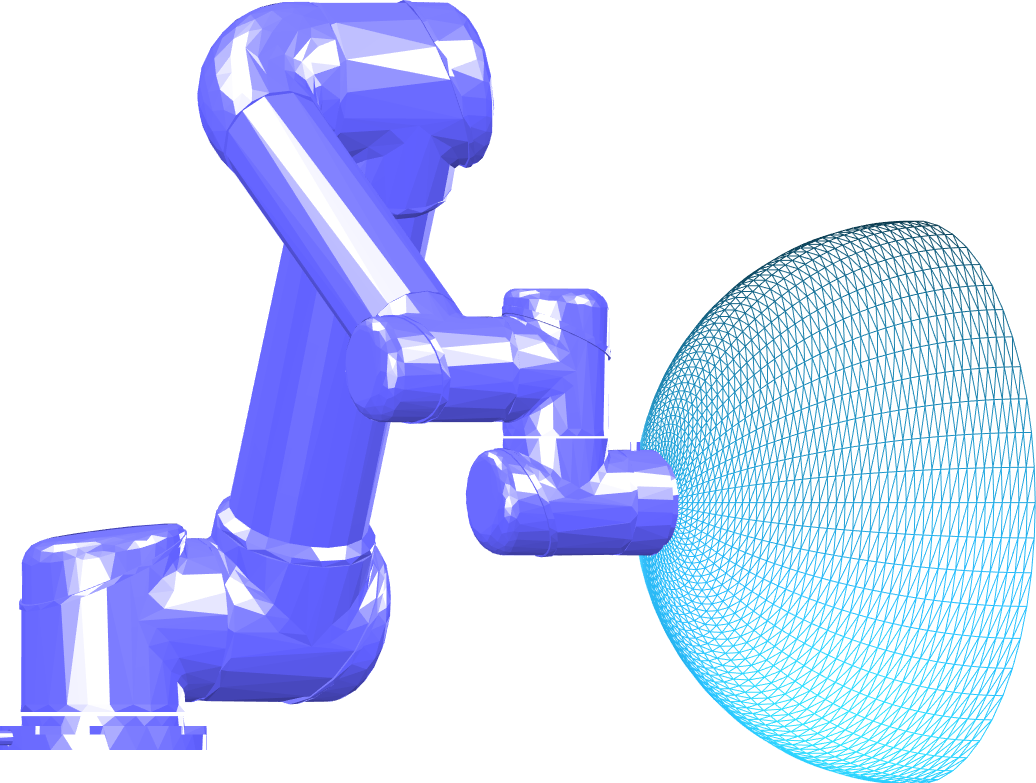
\includegraphics[width = 0.14\textwidth]{figures/other_figures/hemi_demo/center_90}\label{fig:isolated:a}
}
\subfigure[]{
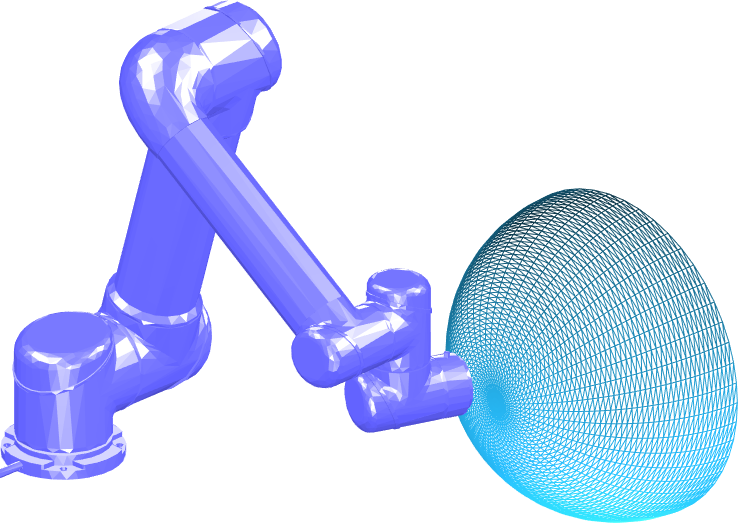
\includegraphics[width = 0.14\textwidth]{figures/other_figures/hemi_demo/offset_90_1}\label{fig:isolated:b}
}
\subfigure[]{
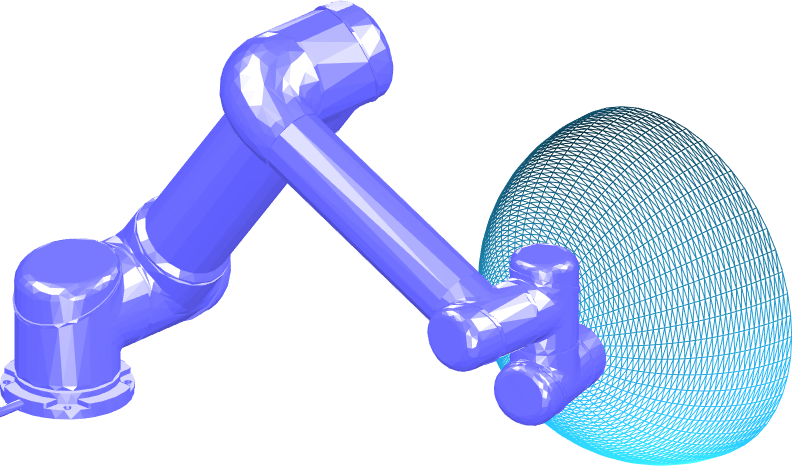
\includegraphics[width = 0.14\textwidth]{figures/other_figures/hemi_demo/offset_90_2}\label{fig:isolated:c}
}
\subfigure[]{
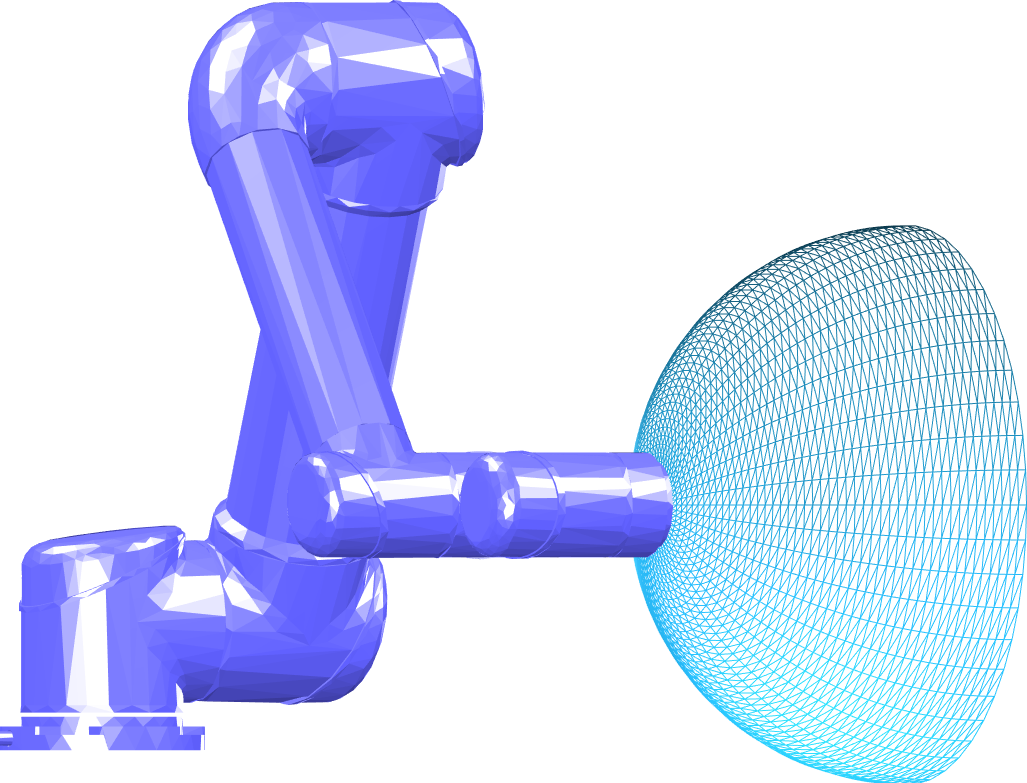
\includegraphics[width = 0.14\textwidth]{figures/other_figures/hemi_demo/center_180}\label{fig:isolated:d}
}
\subfigure[]{
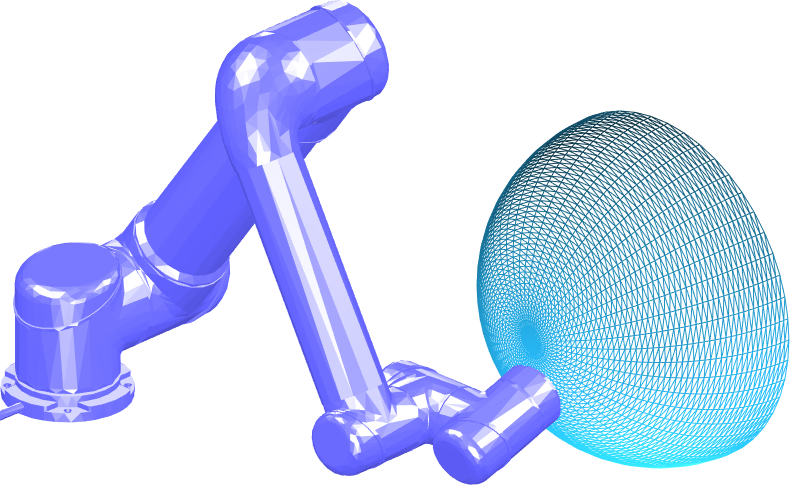
\includegraphics[width = 0.14\textwidth]{figures/other_figures/hemi_demo/offset_180_1}\label{fig:isolated:e}
}
\subfigure[]{
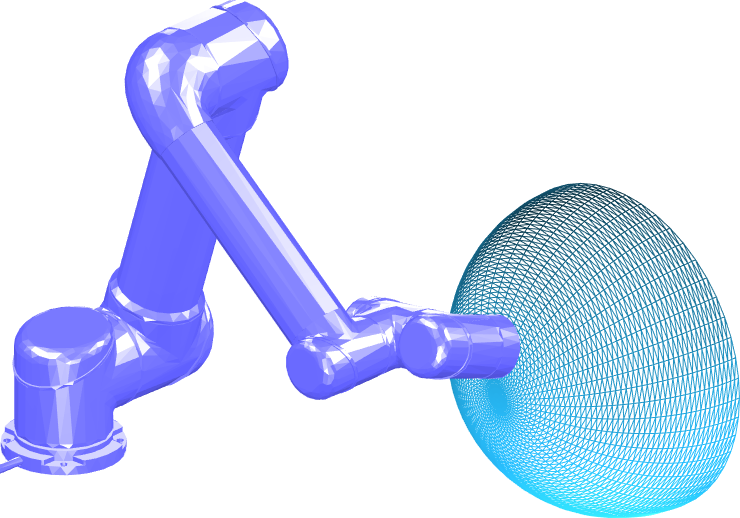
\includegraphics[width = 0.14\textwidth]{figures/other_figures/hemi_demo/offset_180_2}\label{fig:isolated:f}
}
\caption{Illustration of a coverage task with isolated singular point. 
}\label{fig:isolated}
\end{figure}


\begin{figure}[t]
\centering
\subfigure[]{
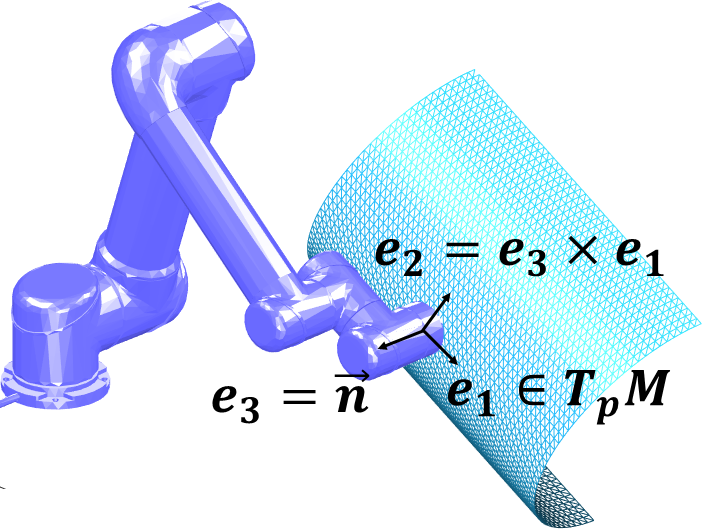
\includegraphics[width = 0.14\textwidth]{figures/other_figures/cylinder_demo/parallel_with_frame}\label{fig:curved:a}
}
\subfigure[]{
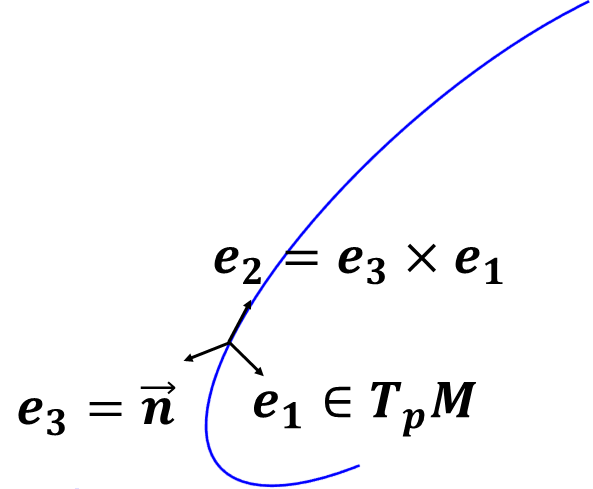
\includegraphics[width = 0.14\textwidth]{figures/other_figures/cylinder_demo/gauss_image_parallel}\label{fig:curved:b}
}
\subfigure[]{
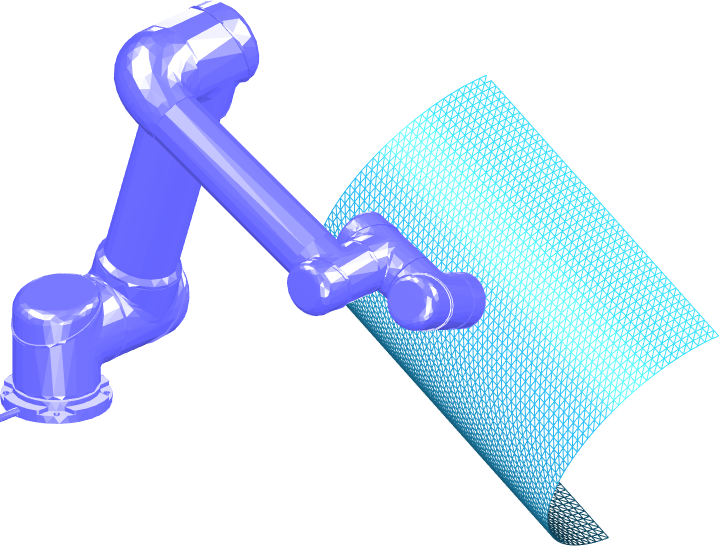
\includegraphics[width = 0.14\textwidth]{figures/other_figures/cylinder_demo/offset_parallel}\label{fig:curved:c}
}
\subfigure[]{
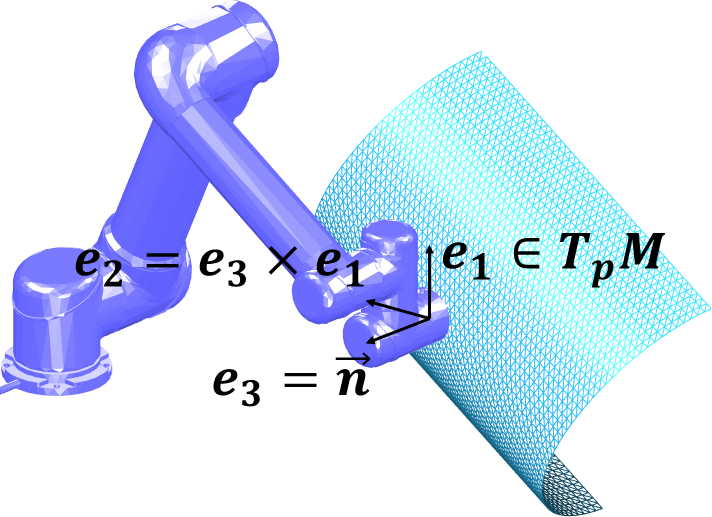
\includegraphics[width = 0.14\textwidth]{figures/other_figures/cylinder_demo/center_90_with_frame}\label{fig:curved:d}
}
\subfigure[]{
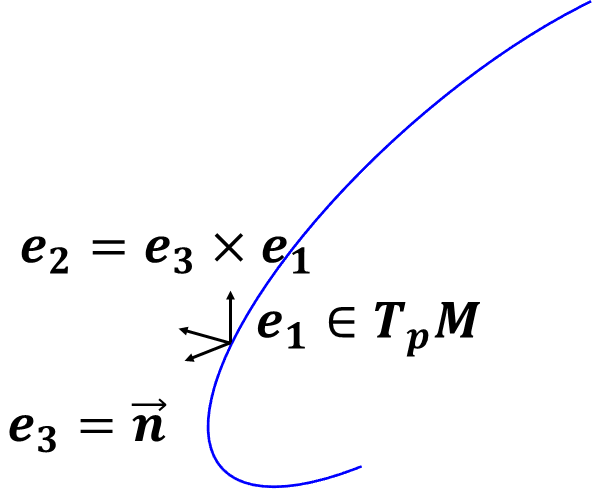
\includegraphics[width = 0.14\textwidth]{figures/other_figures/cylinder_demo/gauss_image_perp}\label{fig:curved:e}
}
\subfigure[]{
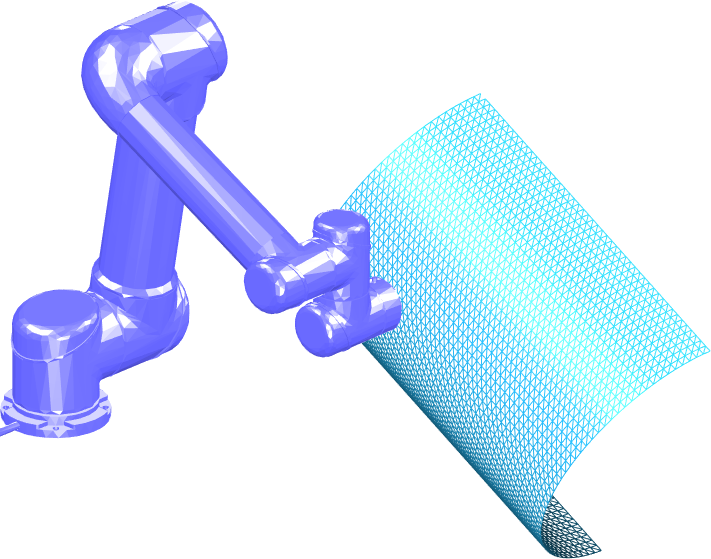
\includegraphics[width = 0.14\textwidth]{figures/other_figures/cylinder_demo/offset_90}\label{fig:curved:f}
}
\caption{Illustration of a curve of singular points where the Gauss mapping is not bijective. 
}\label{fig:curved}
\end{figure}

On one hand, let the Gauss mapping around $x$ be bijective.
For any path $\gamma$ on the sphere pass $g(x)$, 
\begin{equation}\label{equ_gamma}
\forall \gamma: [-1, 1]\rightarrow \mathbb{S}^2, 0\mapsto g(x)
\end{equation}
satisfying that its tangent at $g(x)$ is restricted to 
\begin{equation}\label{equ_gamma_direction}
\frac{d\gamma(s)}{ds}|_{s = 0} // g_*(e_2)
\end{equation}
we can always find its preimage, a path $\gamma_M$ on the surface, satisfying that 
\begin{equation}\label{equ_gammam}
g(\gamma_M) = \gamma\Rightarrow \gamma_M = g^{-1}(\gamma)
\end{equation} 
Then $\gamma_M$ is a permissible path that is smoothly traversable because $g_*$ is a homogeneous tranformation, 
\begin{equation}\label{equ_gamma_para}
\frac{d(g^{-1}(\gamma(t)))}{ds}|_{t = 0} // e_2
\end{equation}
which means that the instant motion of the EE tracking $g^{-1}\comp\gamma$ need not rotate about $e_2$. 
So a workspace coverage path is smoothly traversable as long as we precisely design the tangent of the coverage path to satisfy (\ref{equ_gamma_para}). 

On the other hand, the preimages of a same Gauss image have parallel unit outer normal vectors, the motion between whom does not require any rotational motion. 
So if the Gauss mapping is not bijective at point $x$, a joint-space path of pure translational motion can be inserted in the result path taking the place of $g^{-1}(\gamma(0))$, i.e., between
\begin{equation}
g^{-1}(\gamma([-1, 0)))\mbox{ and }g^{-1}(\gamma((0, 1])))
\end{equation}
and the doability is guaranteed by the translational manipulability. 
Hence, if the surface has a locally planar region (curve) around $x$ that allows pure translational motion, besides $\gamma_M$ constructed as above, the EE may alternatively choose any coverage path within the planar region. 


For example, in Fig. \ref{fig:isolated} there is a singular point in the center of a wok-like object, because when the EE is covering the central point, the $2$-nd, $3$-rd and $4$-th joints of the manipulator are rotating in a same 2D plane, as shown in Fig. \ref{fig:isolated:a} and Fig. \ref{fig:isolated:d}. However, it is easy to verify that they are still valid in the sense of translational manipulability. 
The surface is part of a sphere, so the Gauss mapping is equivalent to shrinking the surface to the unit sphere. The configurations shown in Fig. \ref{fig:isolated:b} and Fig. \ref{fig:isolated:c} are the continuous configurations that are smoothly traversable from the one shown in Fig. \ref{fig:isolated:a}, from which the EE can only move horizontally. 
And Fig.\ref{fig:isolated:e} and Fig.\ref{fig:isolated:f} are continuous to Fig.\ref{fig:isolated:d}, from which the EE can only move vertically. 

Another example is shown in Fig.\ref{fig:curved}. 
The object is part of a cylinder, whose unit normal vectors are parallel along the generatrix, so the Gauss image is only an arc in the unit sphere. 
When the manipulator is at a singular configuration like shown in Fig.\ref{fig:curved:a}, the $g_*(e_2)$ axis is tangent to the Gauss image of the cylinder, so the manipulator is able to perform motion in two dimensions, along the generatrix (through pure translational motion of EE) and perpendicular to the generatrix (shown in Fig.\ref{fig:curved:c}). The case remains the same if the wrist joint flips exactly $\pi$ rad. 
However, for other valid singular configurations such as the one shown in Fig.\ref{fig:curved:d}, it is easy to see that the manipulator cannot track any path with nontrivial Gauss image on the semicircle, because all of them have non-zero projection on the $g_*(e_1)$ axis, thus require rotational motion about the $g_*(e_2)$ axis. However, the EE can still move along the generatrix which requires only translational motion, as shown in Fig.\ref{fig:curved:f}. 


\subsection{Existance of Non-Pausing Motion}
Notice that in (\ref{equ_total}) $\bar{N}$ is not necessary to be $\bm{0}$. 
When
\begin{equation}\label{equ_notzero}
\bar{N}\cdot \bar{\omega}^\perp = \sum\limits_{i = 1}^5 \bar{N}_{1i}\bar{V}_{i5}\hat{\omega}_5 \neq 0
\end{equation}
the null motion changes the manipulator configuration with the 5D pose of the EE remaining static, i.e., rotating about the $e_3$ axis. 
%Note that whether (\ref{equ_notzero}) is non-zero depends on the singular configuration that the manipulator is currently at. 
Rotating about $e_3$ means changing the direction of $e_1$ and $e_2$ in the tangent plane of the surface, hence the application of the null motion indirectly yields another dimension of motion at the singular point.  

Combining the motion along the permissible path and the null motion, we claim that the EE never has to suspend at the singular point. 
When there is a curve of singular points the EE obviously need not suspend, because the manipulator can always adjust its configuration while performing translational motion among singular points. 
The case of isolated singular point is also easy to prove. 
Given any valid singular configuration $c$, recall that the task constraints are given by strict inequalities. 
Even if the instant motion has been restricted to a specfic orientation, as long as there exists a permissible path $\gamma_M: [-1, 1]\rightarrow M$, $\gamma_M(0) = x$, there must exists a small open interval $(-\delta, \delta)$ such that all IK solutions to cover $\gamma_M((-\delta, \delta))$, which are continuous to $c$, satisfy all task constraints. 

%\end{color}

%For example, in the hemisphere example, we use a twisted surface as the visualization of valid configurations in covering the central part of the object. 
%See Fig.\ref{fig_structure_demo_1} and Fig.\ref{fig_structure_demo_2} for illustration of the distribution of valid regular configurations and all configurations. 
%The horizontal coordinate of each point in the twisted surface is the EE position of the corresponding configuration on the surface, and the height coordinate is set to be the angle value of the $4$-th joint. 
%At any point on the object other than the central point, there are only finite number of image points, while at the central point there are infinite many image points. 
%At the central point, through null motion, the manipulator can traverse to any height, which however requires the suspension of the EE at the central point. 
%Hence, although at any height, the intersection between the image surface and the horizontal plane is just a line, as long as the coverage path is smooth when passing the singular point, the EE need not suspend on it. 

%We can see from Fig.\ref{fig_structure_demo_2} that the configurations belonging to different colours are connected with the usage of the singular configurations, which makes two colours become a single one. Although the colour distribution is folded in the task-space, in analytic surface the choice of configurations to continuously track a given coverage path is still well-defined, because at any valid configuration the traversable direction in the joint-space is two-dimensional. 
%However, in discretized mesh, how to choose the correct continuous adjacent configurations becomes a big problem, which is the main focus of the next section. 


%\begin{figure}[t]
%\centering
%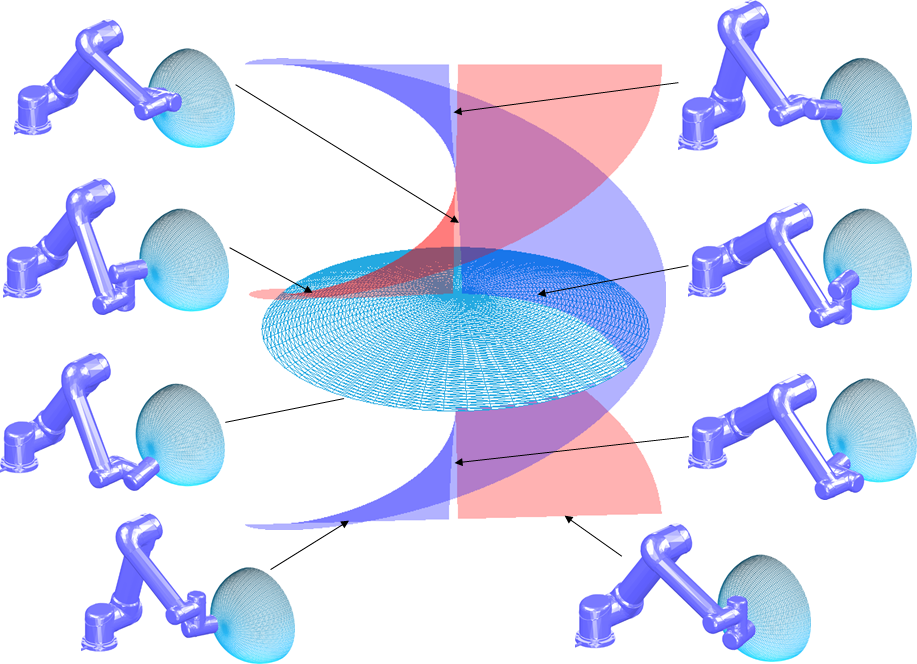
\includegraphics[width = 0.44\textwidth]{figures/other_figures/structure_demo_1}
%\caption{Illustration of the valid configurations to cover near but excluding the singular point. Note that the top part and the bottom part of the helicold structure correspond to same configurations, so the distribution of the blue (or red) configurations is like a mobi\"{u}s strip (here we omit other constraints, such as the collision avoidance, considering which may cut off the strip). 
%For better illustration, we omit doing collision detection between the wrist and the fore-arm. }\label{fig_structure_demo_1}
%\end{figure}
%
%\begin{figure}[t]
%\centering
%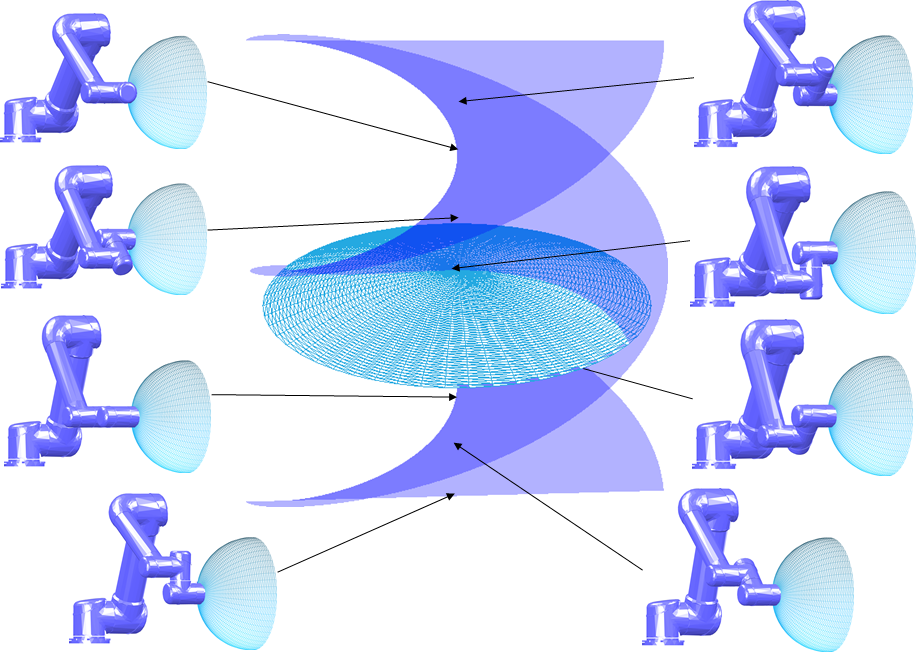
\includegraphics[width=0.44\textwidth]{figures/other_figures/structure_demo_2}
%\caption{Illustration of the valid singular configurations that covers the singular point required in Fig.\ref{fig_structure_demo_1}. After envolving the valid singular configurations, the manipulator can freely transit from a ``red" configuration to a ``blue" configuration, i.e., they are merged to a single color. }\label{fig_structure_demo_2}
%\end{figure}

%\subsection{Construction of Topological Cells}
%Since the only concern about smooth visiting the singular point is the motion direction of the coverage path, we may adopt the polar representation in the local coordinate around the singular point. Then we can refer to different configurations by their position in the polar coordinate. 

%Following the criterion of constucting topological cells and based on the assumption of this paper that the surface is analytical, after we collect some valid singular configurations, 

%Theoretically, when the forward kinematic mapping from the joint space to the work space is non-bijective, it is also a non-homemomorphic one, then the cell is no longer boundary-free. 
%A simple example is shown in 


\subsection{Summary of Results and More Generalization}
In summary, no matter how many degrees of freedom that the non-redundant manipulator has, since the EE motion on the surface of the object is a 2D one, if the manipulator is in a valid singular configuration under rank-deficient manipulability constraints, losing the capability of the EE moving in one dimension means there is only one dimension left, leading to a restricted motion direction of the coverage path on the singular point. Thus through properly design the motion direction of the EE when passing the singular points, the manipulator can smoothly track the coverage path without EE lift-off or suspension. 

%From another perspective, passing through singular points may lead to smooth transition between configurations which belong to different colours when overlooking the singular configurations. So if possible we should always consider visiting the singular point to avoid EE lift-offs. 

\begin{color}{blue}
\section{SNCPP in Discretized Data}\label{section_discrete}
\end{color}
It is noticable that the singular points only form zero-area region on the target surface. If we finitely sample some waypoints or do CPP on the vertices of a triangular mesh, there is zero probability to know the exact position of the singular points. 
On a side note, it also means that some ``sampling in manifolds" algorithms for path planning task is unapplicable, because the structure of bifurcation cannot be properly modelled. 
What makes the problem become more complex is that we can neither leverage the null space path during planning, because following a ``designing-tracking" scheme the coverage path is designed on the surface, where a null space path only corresponds to a single EE point. 
We observe that two consecutive waypoints indicate a straight path connecting them, so even if we cannot find the singular point, the coverage path may still pass it as long as two waypoints stay opposite to it. 

In this section, we present the necessary and sufficient condition to leveraging singularities without precise knowledge about their position, and proposed a practical strategy to both leveraging the singularities and adapting conventional CPP solutions. 
%From another perspective, we are designing a sampling strategy to construct an appropriate mesh enabling the usage of the singularities. 

\begin{figure}[t]
\centering
\subfigure[]{
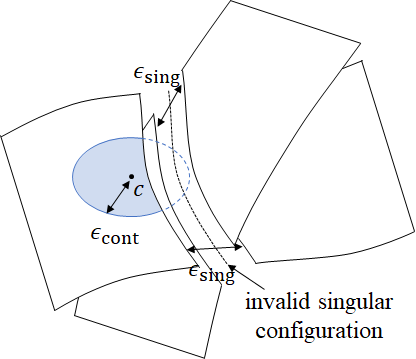
\includegraphics[width=0.22\textwidth]{figures/other_figures/cspace_gap}\label{fig:gap:a}
}
\subfigure[]{
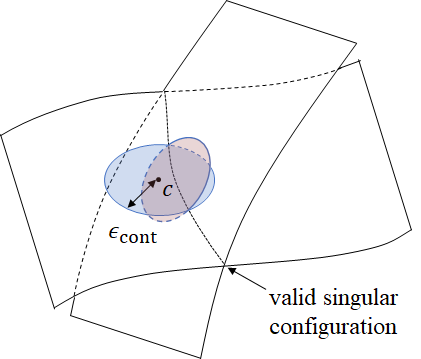
\includegraphics[width=0.22\textwidth]{figures/other_figures/cspace_nogap}\label{fig:gap:b}
}
\caption{Illustration of the valid configurations near singularities. If the singular configuration cannot satisfy the manipulability constraint, then a gap exists between the singular configurations and the valid configurations with width $\epsilon_{\rm sing}$. For $\epsilon_{\rm cont} < \epsilon_{\rm sing}$, regarding $\epsilon_{\rm cont}$ as a threshold of judging the continuity of configurations, the algorithm always performs correctly. However, for the valid singular configurations, there does not exist such a gap, thus for any precision of $\epsilon_{\rm cont}$, the algorithm will inevitably make mistakes.
}\label{fig:gap}
\end{figure}

\begin{figure}[t]
\centering
\subfigure[]{
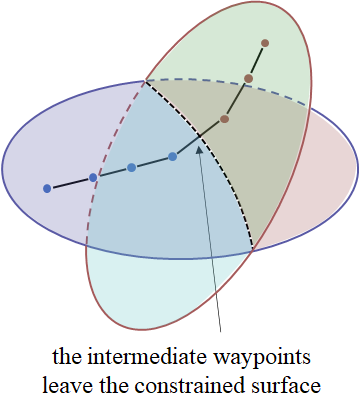
\includegraphics[width=0.22\textwidth]{figures/other_figures/demo_planning_path}
}
\subfigure[]{
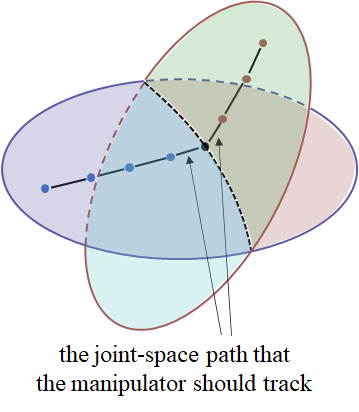
\includegraphics[width=0.22\textwidth]{figures/other_figures/demo_controlling_path}\label{fig:indicated:b}
}
\caption{Without the singular configuration as a waypoint, the indicated joint space motion given by the CPP planner is not trackable. The tracking problem will be solved by the low level controller, but then the coverage path will requires null motion which means EE suspension on the surface. 
}\label{fig:indicated}
\end{figure}

\begin{figure}[t]
\centering
\subfigure[]{
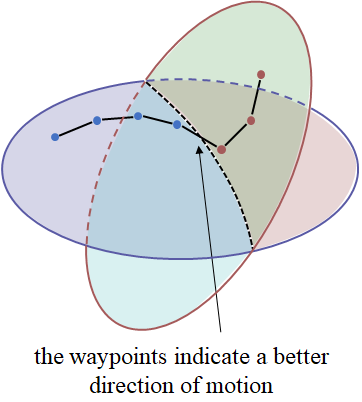
\includegraphics[width=0.22\textwidth]{figures/other_figures/demo_better_planning_path}
}
\subfigure[]{
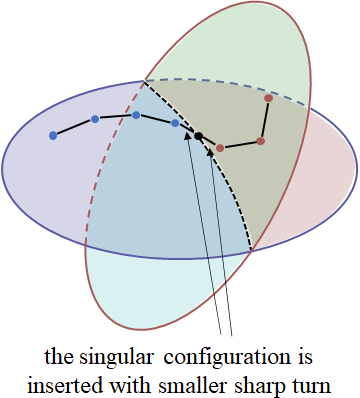
\includegraphics[width=0.22\textwidth]{figures/other_figures/demo_better_controlling_path}
}
\caption{Illustration of a better solution of the case in Fig.\ref{fig:indicated}. Although the coverage path neither contains the singular point, the motion orientation of the two waypoints vary, which makes the indicated straight path closer to the singular point. Then after the path be optimized to a continuous trajectory by a low-level controller, it contains a smaller sharp turn. Ideally, there exists one motion direction (the permissible path discussed in Section \ref{section_analytic}) that the straight path implicitly passes the singular point, then there is no sharp turn in the optimized joint-space trajectory. 
}\label{fig:better}
\end{figure}

\subsection{Why EE Suspending}
When the algorithm deals with discrete data and cannot capture the singular point, it has to use a discrete distance threshold to label the continuous configurations, such as
\begin{equation}\label{equ_continuous}
\forall c_1, c_2\in \mathscr{C}, c_1, c_2\mbox{ are continuous}\Leftrightarrow d(c_1, c_2) < \epsilon_{\rm cont}
\end{equation}
where $d(\cdot, \cdot)$ can be the joint-space distance, and $\epsilon_{\rm cont} > 0$ is a pre-determined joint-space distance threshold. 
$\epsilon_{\rm cont}$ depends on the resolution of the mesh and $\epsilon_{\rm sing}$. 
When the mesh is of higher quality, the configurations covering adjacent vertices on the mesh have smaller joint-space difference, which is good for judging continuity. 
However, for sparse mesh, $\epsilon_{\rm cont}$ has to be a little bigger so that two discrete but essentially continuous (without passing singularity) configurations can be still correctly seen as continuous. 
And $\epsilon_{\rm cont}$ should be less than $\epsilon_{\rm sing}$ so that the algorithm would not mistakenly see two configurations (passing invalid configurations) as continuous. See Fig.\ref{fig:gap:a} for illustration. Note that $\epsilon_{\rm sing}$ is in an implicit form, so $\epsilon_{\rm cont}$ is chosen as small as possible. 
(This also means that the mesh cannot be too sparse, or else no suitable $\epsilon_{cont}$ can be found: either some continuous configurations are assigned with different colours, or some discontinuous configurations are given same colour.)
However, it is noticable that when there exist valid singularities, no matter how small $\epsilon_{\rm cont}$ is, it will always make wrong judgement, because the singular configurations between different continuous sets have zero-area, i.e., $\epsilon_{\rm sing} = 0$. See Fig.\ref{fig:gap:b} for illustration. 
We claim that the algorithm will come up with correct result, i.e., cellular decompositions, but will give inappropriate coverage path. 

The reason of having correct results is that, although we have zero possibility to sample the singular point $x$, we have non-zero probability to find two configurations, one in each colour, which are close enough (with distance less than $\epsilon_{\rm cont}$). 
For example, denote the singular configuration to cover the singular point $x$ as $s$ which is sub-resolutional. We can always find two configurations $c_1$ and $c_2$ near $s$ belonging to different colours. They are so near that 
\begin{equation}\label{equ_near}
d(c_1, s) <\frac{\epsilon_{\rm cont}}{2}\ \&\ d(c_2, s) < \frac{\epsilon_{\rm cont}}{2}
\end{equation}
then 
\begin{equation}
\begin{aligned}
&d(c_1, c_2) < d(c_1, s) + d(c_2, s)<\epsilon_{\rm cont}\\
\Rightarrow &c_1, c_2 \mbox{ are thought to be continuous} 
\end{aligned}
\end{equation}
Since the algorithm will be only ``mistakenly connecting" but no ``mistakenly disconnecting", when the SNCPP problem is modelled with finite but dense discrete mesh, even without capturing the valid singular configurations, the optimal number of EE lift-offs and the optimal cellular decompositions are automatically correct results. 

But we also claim that the coverage path would be almost surely false. It is intuitive following the illustration in Fig.\ref{fig:indicated}, where the straight path connecting two waypoints (configurations) is off the constrained manifolds. In other words, the path planner does not provide a trackable solution for the subsequent low-level trajectory generator. 
However, this is all what the planner can do. 
And in the subsequent controlling stage, a controller might have a more precise model about the local distribution of the valid configurations (maybe an analytic model of the surface), and thus may be able to optimise the untrackable path gradually onto the constrained manifolds and generate speed commands. And following the discussion in Section \ref{section_analytic}, a singularity must lie in the optimized trajectory. 
Since the path did not indicate a smooth transition between colours, a conventional trajectory optimizer will finally add a sharp turn at the singularity, as shown in Fig.\ref{fig:indicated}. 
If the planner could have provided two consecutive waypoints that are almost aligned with the permissible direction of smoothly visiting the singularity, then after the indicated joint space path being modified by the controller, the angle variation at the sharp turn would be smaller, which requires less null motion. See Fig.\ref{fig:better} for a better coverage path indicated by discrete waypoints. 


\subsection{Condition for Asymptotically Optimal Solutions}\label{subsection_asymptotical}
We claim that the necessary and sufficient condition of leveraging singular points on discretized data structure is that, the sampling strategy is asymptotically finding all elements in the unit tangent bundle of the surface. Here the unit tangent bundle is the set of all unit tangent vectors of all points on the surface $M$, denoted by $UM$, which is a 3D space. 

The sufficiency is intuitive to show if we regard the waypoints of the coverage path as the elements in $UM$, i.e., each waypoint possesses the instant motion direction when the EE passes it. 
From the previous discussion we know that the only constraint when passing the singular point is the restricted motion orientation, so given any non-zero smoothness criterion of the joint space path, we can find an element arbirarily close to the desired ``singular point position -- permissible direction" pair. 

The proof of necessity is also easy through constructing a counterexample. If there exists a point on the surface in which unit tangent space is not asymptotically completely sampled, then we may precisely choose a pose of the object to put this point to EE position of a singular configuration with the permissible orientation be just overlooked by the incomplete sampling process. Unable to find a smooth joint-space path visiting the singular point, the result joint-space path has to either perform one extra lift-off if the path planner does not think the two colours are continuous, or perform a sharp turn in the optimized trajectory at the singular point with EE pausing.

\begin{figure}[t]
\centering
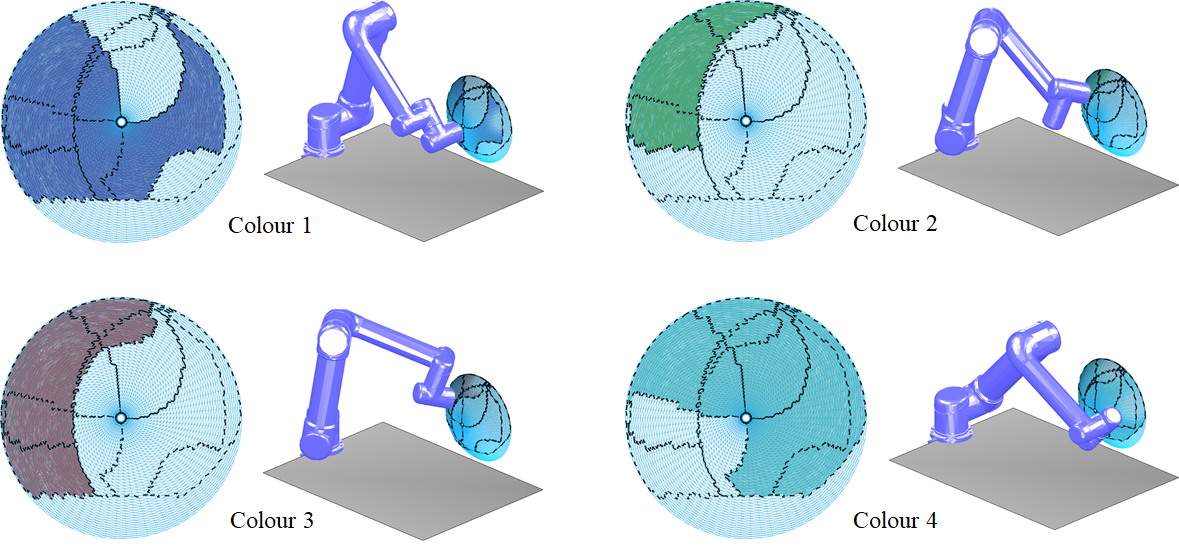
\includegraphics[width = 0.44\textwidth]{figures/exp_central_sphere/ground_truth_demo_color_2}
\caption{Illustration of the examples of available configurations, colour distributions and initial topological graph in covering part of a sphere. 
The singular point is at the center of the mesh. 
In order to visualize all valid configurations, we need the kinematic mapping to be one-to-one, so we remove showing the continuity given by the singular point. 
From the detailed explanation in Fig.\ref{fig:bad_mesh} we know that colour $1$ and colour $4$ are actually continuous when considering the singularities. 
%The mesh is dense, and properly designed near the singular point, so this figure can be seen as the ground truth. 
}\label{fig_ground_truth}
\end{figure}

\subsection{Counterexample of CPP in Non-complete Configuration Set}
In this section we show a counterexample that if the waypoints for CPP are not complete, then the CPP solution cannot leverage the valid singularities to avoid EE lift-offs. We first show a groundtruth solution, and land back to the actual situation on the discrete mesh. 
We again take the sphere as an example. 
For better illustration, we add a ground plane to remove all elbow-down configurations and delete most part of the mesh to focus only on the central part around the singular point. 

The demo of available configurations, colour distributions and initial topological graphs are shown in Fig.\ref{fig_ground_truth}. 
The center of the surface is a singular point following the discussion in Section \ref{subsection_parameterization}, and the EE can smoothly traverse the singularity as long as the instant motion direction does not change, i.e., colour $1$ and $4$ are continuous when considering the valid singular configurations. 
The connectivity of different colours provided by the valid singularities is not shown in this figure, or else the configurations belonging to color $1$ and $4$ would be assigned with a same colour, and the whole graph would be just in a single cell. It is apparent that the optimal number of lift-off is $0$ when considering the singularity: the manipulator covers the left part using colour $1$ and then smoothly transform to colour $4$ through passing the singularity, and finally covers the right part using colour $4$. 
Following are discussion about the algorithm running on discrete mesh. 


\begin{figure}[t]
\centering
\subfigure[IK solutions of vertices when the mesh is sparse. No path planner will regard any two configurations in the figure as continuous, because moving the EE along any of four mesh edges requires much adjustment to the manipulator pose.]{
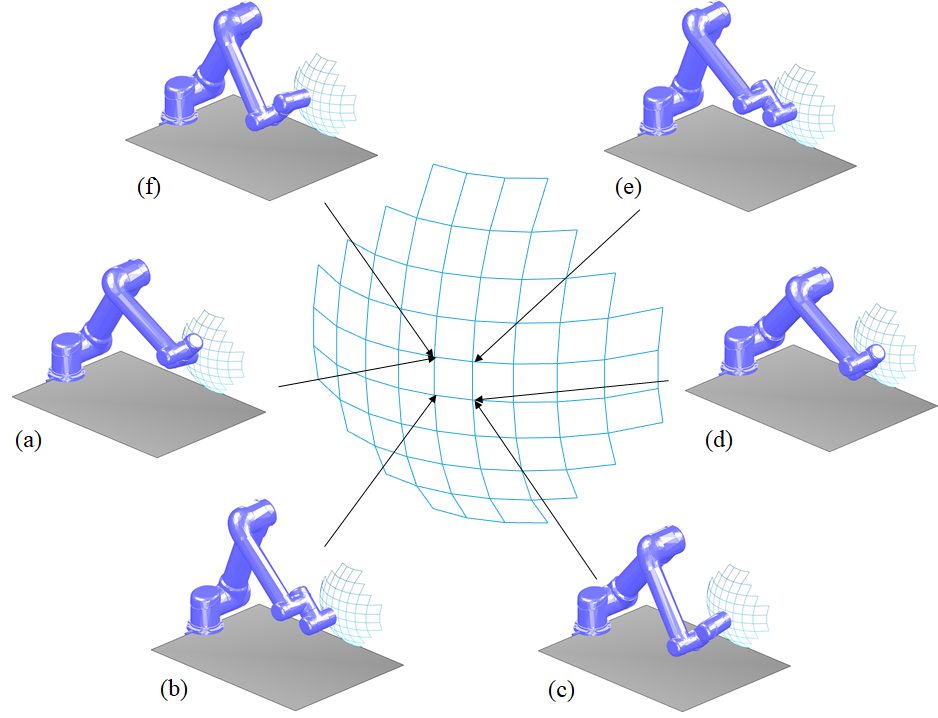
\includegraphics[width = 0.44\textwidth]{figures/exp_central_sphere/sparse_confs_2}\label{fig:nearest:a}
}
\subfigure[IK solutions of vertices after the mesh is refined. (b') and (c') are denoted as the same colour, but it does not mean that the EE can move directly from (b') to (c'). They are continuous because the configurations (g)(h) are inserted as waypoints, which makes (b) and (c) continuous. So (b') and (c') are labelled as a same colour does not necessarily mean that we can arbitrarily design a path connecting (b') and (c') (denoted by a $\times$ in the enlarged figure). ]{
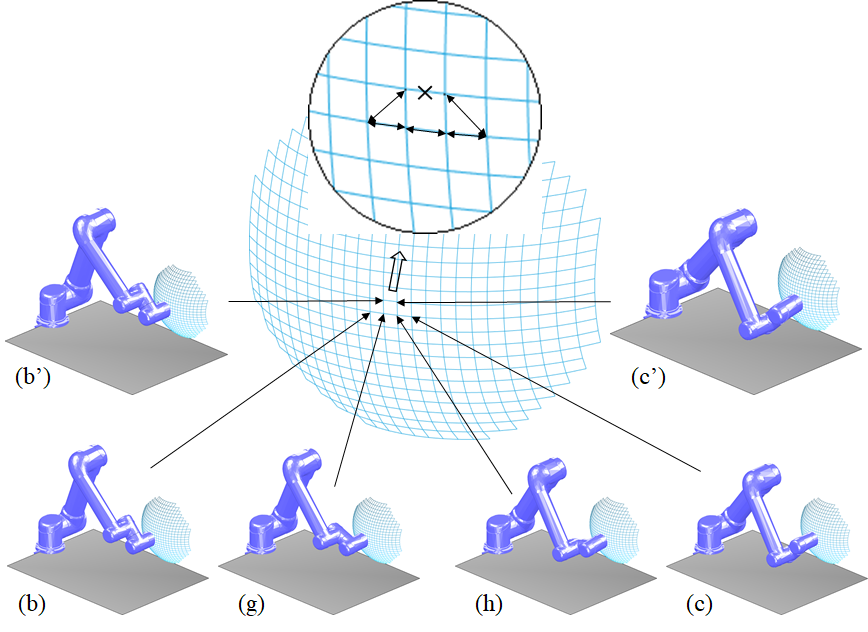
\includegraphics[width = 0.44\textwidth]{figures/exp_central_sphere/sparse_refined}\label{fig:nearest:b}
}
\caption{Illustration of how configurations are connected and how the singularity cannot be leveraged. The colour number follows the definition in Fig.\ref{fig_ground_truth}. }\label{fig_nearest}
\end{figure}

We first show how the algorithm can connect the configurations belonging to a same colour without passing singularity. Let the pattern of mesh be as follows: 
Denote the radius of the sphere by $R$, and the surface is sampled using a planar $n\times n$ grids template, with rising of the vertices in the third dimension. I.e., we first design the vertex $p_{ij}$ on a planar grid, 
\begin{equation}
p_{ij} = \left(\frac{2i-n}{n}R, \frac{2j-n}{n}R\right), i, j = 1, \cdots, n
\end{equation}
a sampling point $\tilde{p}_{ij}$ is chosen as
\begin{equation}
\tilde{p}_{ij} \triangleq \left(\frac{2i-n}{n}R, \frac{2j-n}{n}R, \sqrt{1 - \frac{(2i-n)^2}{n^2} - \frac{(2j-n)^2}{n^2}}R\right)
\end{equation}
$n$ is set as an odd number, so that there is always no vertex that precisely represents the singular point. 
The configurations covering the four nearest vertices to the singular point are depicted in Fig.\ref{fig:nearest:a}, where in such a sparse selection of configurations, no path planner would see them as continuous configurations. However, we can see that (a)(b)(c) are continuous and (d)(e)(f) are continuous as the mesh is refined, see Fig.\ref{fig:nearest:b}. Although the configuration (b')(c') still have huge wrist joint angle difference thus are not considered as directly connectable by the planner, they are assigned with the same colour, because the connectivity goes from (b')$\leftrightarrow$(b)$\leftrightarrow$(g)$\leftrightarrow$(h)$\leftrightarrow$(c)$\leftrightarrow$(c'). 
In this case, if the coverage path planner directly connects of (b') and (c') in the coverage path, a low-level controller can always find the smooth motion with the EE precisely following the edge connecting (b') and (c'), although the wrist joint requires large adjustment since the manipulator path is very near the singularity. 

%Especially, we focus on the colour $1$ configuration of covering the left bottom vertex and the colour $4$ configuration of the right-bottom vertex. 
%From the ground truth result in Fig.\ref{fig_ground_truth}, we know that they are joint-space continuous, but the joint space path contains a null motion during which the EE stays at the singular point.
In contrast to the connection between (b) and (c), now we show how (b) can also connect to (d), a configuration with same EE pose with (c) which breaks the local bijectivity of kinematic mapping assumed in previous works~\cite{Yang2020Cellular}. 
The connectivity is given in Fig.\ref{fig:bad_mesh}, where there is a null motion inserted in between. 
Whenever we simutaneously refine the mesh by adding the same number of horizontal and vertical edges, the four nearest vertices to the singular point are always central symmetric and the four nearest mesh edges form a square, so the connection between (b) and (d) always has a sharp turn of $\frac{\pi}{2}$ rad.  
Obviously, the planner grid has asymptotically captured all points in $X-Y$ dimensions, while it cannot find the connectivity between (b) and (d), thus it becomes a counterexample strategy that is not asympotitally complete to leverage the singularities to avoid EE lift-offs. 

\begin{figure}[t]
\centering
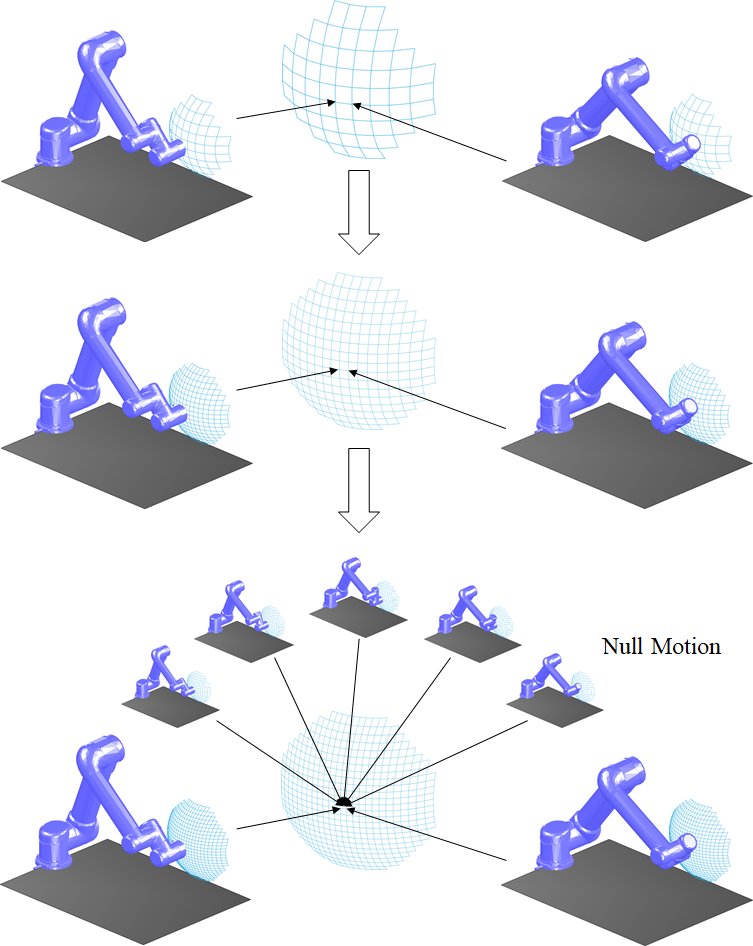
\includegraphics[width = 0.44\textwidth]{figures/exp_central_sphere/pass_to_controller}
\caption{
When the grid is refined both horizontally and vertically, the singular point is always at the center of a square. Hence no matter how precise the mesh is, it does not have a smooth transition of the singular point.  
If the low-level controller is given such two configurations whose straight-path connection is off the surface, assume that it has better local model of the surface, then it might able to gradually optimize the path onto the constrained manifold, i.e., insert the null motion shown in the figure. In this case, the EE lift-off is avoided but EE suspension still exists.}\label{fig:bad_mesh}
\end{figure}

%\begin{figure}[t]
%\centering
%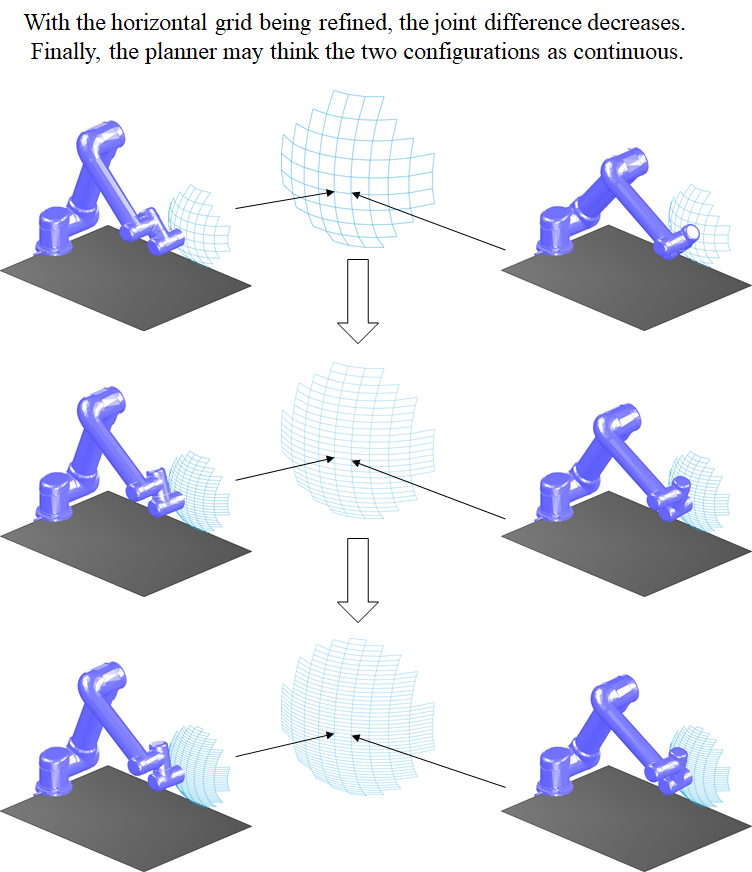
\includegraphics[width=0.44\textwidth]{figures/exp_central_sphere/asymptotically_continuous}
%\caption{Illustration of two configurations which are continuous if we consider the singularities. With the mesh being refined horizontally, the motion between configurations is asymptotical to letting the EE pass the singular point horizontally which is accessible, so we will see that the motion between such two consecutive waypoints looks more and more natural. }\label{fig_asymptotical}
%\end{figure}

%A more interesting example is shown in Fig.\ref{fig_asymptotical}, where we only do horizontal refinement of the mesh but make no changes to the vertical edges. From the figure we can see that the EE is asymptotically able to horizontally visit the singular point without suspension. 
%However, this is just an exceptional case that the singular point is coincidentially traversable horizontally, which is vulnerable given different setting of the SNCPP problem. 
%A simple changing in the environment to show the failure would be adding a tiny obstacle at a precisely chosen position which only abandones the wrist-unflipped configurations (e.g. put it at the wrist position). Since horizontal refinement of the mesh can only capture the horizontal motion visiting the singular point, if horizontal motion hits obstacles thus is unavailable, then the problem of EE suspension still exists. 

In summary, not all discrete representation of surfaces admit a coverage path corresponding smooth EE motion without suspension, and the necessary and sufficient condition for valid discrete representations is proposed and proved in this subsection. 

%\begin{color}{red}
%\subsection{Examples and Counter-Examples of Discrete Representation}\label{subsection_example}
%\noindent
%\indent
%In this subsection we present some examples and counter-examples for refining the surface for sequent geometric CPP solution. 
%
%\textbf{Parameterizing Surface with Grids.} 
%\begin{figure}[t]
%\centering
%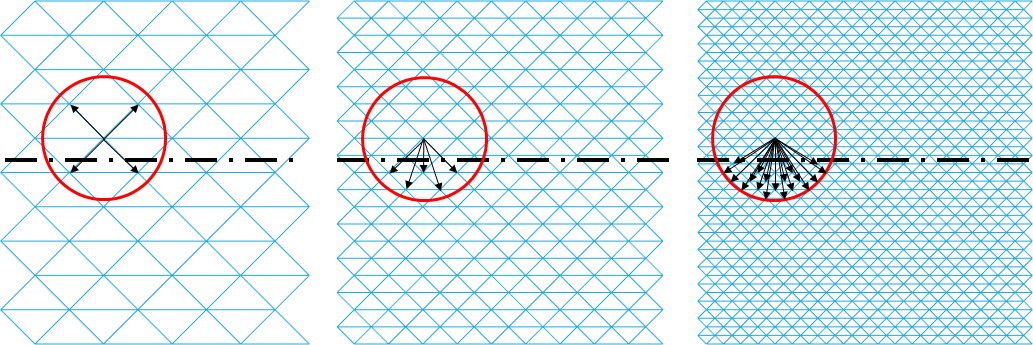
\includegraphics[width = 0.44\textwidth]{figures/other_figures/refine_grid}
%\caption{The connectivity of a vertex using distance based threshold. The singular points is marked in dashed line and the red circle is the distance threshold. As the mesh is refined, the vertex can be connected to more vertices with different motion directions. It is easy to see that the available motion is asymptotical to every direction. }\label{fig_refine_grid}
%\end{figure}
%See Fig.\ref{fig_refine_grid} for illustration. A classical solution of generating triangular mesh on a regular surface (all smooth surfaces are regular surfaces) is first creating the \textit{curvilinear coordinate} of the surface, and then dividing each grid into two triangles. However, at each vertex of the mesh, there are only finite number of orientations that are captured (the basis of the curvilinear coordinate and two $\frac{\pi}{4}$-rad ones), hence, seeing the IK solutions of all vertices as candidates of waypoints and the edges of the mesh as the connectivities between waypoints, it can never find a continuous motion passing the singularities. 
%
%\textbf{Parameterizing Surface with Hexagonal Grid. } 
%We show that it is also improper to parameterize the surface using the hexagonal grids. Such parameterization is always doable because a planar region can be filled in with regular hexagons with arbitrary resolution, and under homeomorphic mapping the 2.5D surface can be also parameterized, as shown in Fig.\ref{} for an example of the hemisphere. The failure is obvious, since there is no waypoints that is passed by a straight segment of path. 
%
%\textbf{Refining the Triangular Mesh by Connecting the Midpoints of Edges. } The simplest method to improve the resolution of a triangular mesh is first creating additional sampling points on the midpoint of each edges, and connecting them to divide the original triangles into four smaller ones, as shown in Fig.\ref{}. However, it is neither applicable because any existing vertex is not connected with new edges, so the orientations passing the vertex is not asymptotically completely sampled. 
%
%\textbf{Refining the Triangular Mesh by Connecting the Incenter. } One of the valid refining strategies of the triangular mesh is connecting the vertices with the incenter of each triangle. The incenter is the intersection of the angle bisectors, hence the newly-added edges will create further sampling on the motion orientation of the existing vertices. Follow a same analysis, the \textit{Barycentric Subdivision}~\cite{} in algebraic topology is also applicable, whose 2D case is that the barycenter is connected to each vertex and each midpoint of edges. 
%
%As a straightforward corollary, purely random sampling on the surface combining with distance-based connectivity is always a valid strategy. 
%\end{color}

\subsection{Practical Solution to SNCPP in Discrete Mesh}
\begin{figure}[t]
\centering
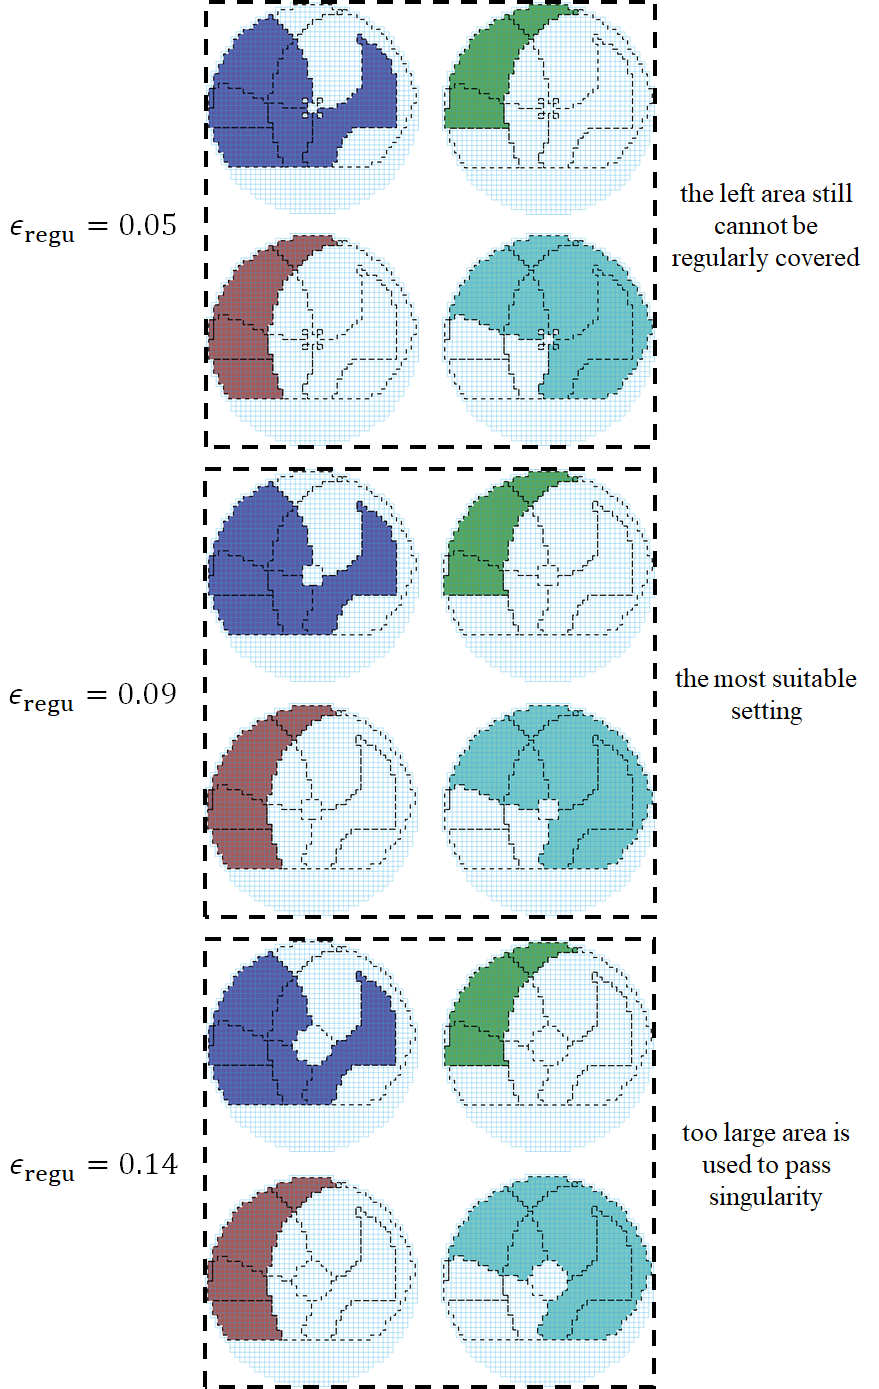
\includegraphics[width = 0.48\textwidth]{figures/exp_central_sphere/choose_threshold_2}
\caption{Illustration of different $\epsilon_{\rm regu}$ for assigning a most suitable region for passing the singularity. It depends on the configuration continuity threshold $\epsilon_{\rm cont}$. 
Having chosen the value of $\epsilon_{\rm cont}$, whatever value it is, since the joint-space near singularity is not flat, the continuity is always wrongly judged. $\epsilon_{\rm regu}$ is set to split those irregular configurations and other configurations which can be connected through template coverage paths. 
$\epsilon_{\rm regu}$ actually prevents some configurations from being chosen in template coverage path, so it should be as small as possible. 
In this example, $\epsilon_{\rm regu} = 0.05$ is not enough, because there are still four configurations that cannot be judged as continuous to adjacent configurations, i.e., they cannot be used as waypoints of template coverage paths. 
(We omit showing the demos of manipulator configurations here, and the reader is referred to the associated video for the visualizations.)
$\epsilon_{\rm regu} = 0.14$ is a valid parameter, however, it splits too many configurations, reducing the region that could have been covered by template paths. In contrast to $0.05$ and $0.14$, $\epsilon_{\rm regu} = 0.09$ is a better setting. 
}\label{fig:choose_threshold}
\end{figure}

\begin{figure}[t]
\centering
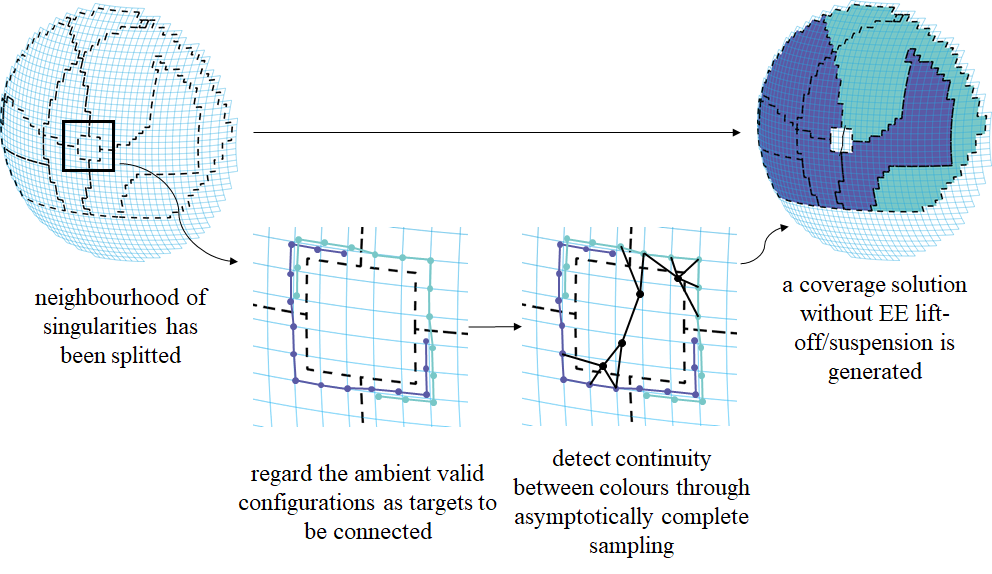
\includegraphics[width = 0.48\textwidth]{figures/exp_central_sphere/complete_sampling/complete_sampling}
\caption{Concept of asymptotically complete path finding in the splitted area. Points with different colours mean different IK solutions to cover the mesh vertices. The configurations to be connected are naturally symmetrical around the singularity, so the desired connection is actually easy to find. After the black path is planned, the coverage task for this object requires $0$ EE lift-off. }\label{fig:complete_sampling}
\end{figure}

As a simple corollary to the result in Section \ref{subsection_asymptotical}, ``pure ramdom sampling with distance-based continuity" is obviously a valid strategy to select EE poses asymptotically ensuring smooth passing singularities. However, if the waypoints are not regularly sampled, such as using the template grids, then conventional coverage path solution (e.g. the back-and-forth path) cannot be easily adapted. Doing CPP on a non-regular mesh is equivalent to put a Travelling Salesman Problem (TSP) problem to the geometric coverage path planner, which is undesired in realistic application. 
Recall that in Section \ref{subsection_all_finiteness} we have splitted the whole surface $M$ into two parts, 
\begin{equation}
M = \bar{M} \cup \left\{\bigcup\limits_{\lambda\in \Lambda}B(x_\lambda, \delta_{x_\lambda})\right\}
\end{equation}
where $\bar{M}$ can be covered with full non-singular configurations, and the last term goes to infinitely small to make $\bar{M}$ and $M$ having same surface area. This motivates us to practically assign a small piece of joint-space region specially for leveraging the singularities, whilst other region can be covered through regular template coverage path solutions, such as the boustrophedon path. 
Following this idea, we split the valid configurations into two parts. One part consists of configurations near the singularity, which cannot be leveraged by a template coverage path designed on the task-space, while another part consists of configurations where the manipulator kinematic mapping is relatively ``flat" so templated coverage paths can be applied. 
$\epsilon_{\rm regu}$ is adapted to be the threshold. 
Within the $\epsilon_{\rm regu}$-neighbourhood of the valid singularity, we try obtaining connectivity among the surrounding non-singular configurations. The configurations are symmetrically distributed to the singularity, thus are pairwise likely to be connected, so such connectivity is easy to get. 
See a concept map in Fig.\ref{fig:complete_sampling}. 
Sampling-based planners (such as the RRT*~\cite{Karaman2011Sampling} algorithm) can be easily adapted to asymptotical completeness and we omit further description. 

In our case, through analyzing the kinematic of the manipulator, we know that valid singularities appear when the $5$-th joint angle equals to $0$ or $\pi$ rad, so $\bar{M}$ is constructed as long as the configurations with 
\begin{equation}\label{equ_remove_neighbour}
\omega_5\in [-\epsilon_{\rm regu}, \epsilon_{\rm regu}]\cup [\pi-\epsilon_{\rm regu}, \pi+\epsilon_{\rm regu}]
\end{equation} 
are removed. 
The colour distribution in the hemisphere case after splitting the neighbours of singularity are depicted in Fig.\ref{fig:choose_threshold}. Since all colours have access to the singularity, all of them are splitted a little near the singularity, making the central part of the surface uncoverable by template coverage paths. It is just a coincidence and not always the case. Later we will show in Section \ref{subsection_realworld} that some singular points can be covered by other non-singular configurations. 

For a visualing illustration of choosing an appropriate $\epsilon_{regu}$, see Fig.\ref{fig:choose_threshold}. Note that it is not our focus to finding the optimal parameter $\epsilon_{regu}$ for a concrete object, or choosing different optimal parameters for different singularities on the object. We concentrate on how to simultaneously applying conventional solutions for the CPP task and leveraging the valid singularities, and the proposed strategy works for this. 

\subsection{Summary}
In Section \ref{section_analytic} and \ref{section_discrete} we face with the problem of adapting valid singular configurations in the SNCPP problem, which makes the mapping from valid configurations to task space regions to be non-bijective, and the coverage path in cells becoming non-arbirarily designed. 
Seeing that the singularities only form zero-area region, we prove the finiteness of cells in the graph. We prove that the transition between colours on the surface is applicable when passing singularities, and a non-stopping smooth EE motion can be established if it goes in the permissible direction when passing singular point. 
For discretely represented surface meshes, we propose necessary and sufficient condition for the waypoints selection to implicitly pass the singularities without a mesh vertex staying exactly on the singular point. A practical method is proposed to simultaneously leverage singularities and template coverage paths.  

Eventually, even if the colours in the SNCPP problem becomes non-bijective, the problem can still be completely separated into two independent stages, the optimal cellular decomposition stage and the coverage path designing and tracking stage. 
Hence the solution of the SNCPP problem can still land back to discussion on solving all kinds of topological graphs.

\begin{color}{blue}
\section{Preliminary Results about the Solutions}\label{section_preliminary}\label{section_simply_connected}
\subsection{Topological Cellular Decomposition}
Given the initial topological graph, the output result can be seen as a colouring scheme that specifies each point one of its available colours. The common boundary between two regions of different colours is called a cutting path. 

The optimality of the cellular decomposition is ``topological" because, compared with the cutting paths of other cellular decompositions in the conventional sense, such as the sweeping lines used in the Trapezoidal Decomposition~\cite{Seidel1991Simple}, the only optimality that our cellular decomposition keeps is the number of continuous sets of different colours constructed by the cutting paths to be the minimum. 
Even if the position and shape of cutting paths vary, as long as the topological (connectivity) structure of the colouring scheme does not change, the cellular decomposition remains optimal. 


\subsection{Homeomorphic Mapping and Classification of Surfaces}
\noindent
\indent
Homeomorphic mapping is a continuous, invertible mapping between two sets. The homeomorphism means the equivalence in the shape of surfaces. As in our case, the surface of any 3D object will always become a 2.5D one by adding cut loci, and is then homeomorphic to a 2D canonical region. And it is well known~\cite{Simmons1964Introduction} that the planar regions are classified into different categories through their genus, i.e., the number of holes within the outer boundary. So in order to cover all situations of cells appeared in realistic application, we only need to consider the solution of cells with all genus. Especially, under homeomorphic mapping, the discussion can be safely splashed on standard unit discs, concentric rings, etc.  

\subsection{All Optimal Solutions}
\noindent
\indent

The output of the proposed algorithm is ``all optimal cellular decompositions". 

Obviously, there are infinite number of different optimal cellular decompositions. 
By adapting the terminology ``topological", we regard different cellular decompositions whose cutting paths are homotopic~\cite{Simmons1964Introduction} as a single type of topological cellular decomposition, which is equivalent to making a \textit{quotient space} to the space of all optimal solutions under the equivalent condition of homotopic modification of cutting paths. 
However, even so, there are still infinite number of elements in the quotient space. 
The only way to obtain all optimal solutions is to keep finding equivalent cellular decompositions in the sense of same number of lift-offs, i.e., find more equivalent conditions to create a smaller quotient space. After finding enough number of equivalent conditions, the quotient space is so small that it is proven with only finite number of elements. Then, any enhausted strategy will collect all optimal solutions as desired. The solution being enumerated is a representative of all other cellular decompositions in the same equivalent class, hence all optimal solutions are collected. 

\subsection{Complexity of Algorithms}
In the proposed algorithm, the cell is solved one by one, so as long as the solution of one cell is not of constant complexity, the overall complexity is always exponential. Thus we do not care much about further reducing the coefficient of the exponential function, but focus on proving the finiteness of the solving process and showing the mechanism to assure all optimal solutions. 
Although there may exist more efficient algorithms that come up with one optimal solution with lower algorithmic complexity, we argue that finding all solutions performs more heuristic to the community. 
Conversely, counterexamples can be easily constructed to show that the exhausted strategy in the quotient space is necessary to assure all optimal solutions. 




\subsection{Solutions of Simply-Connected Cells}
\begin{figure}[t]
\centering
\subfigure[Example shows that it is sufficient to consider cutting path which starts and end at the topological edge endpoints.]{
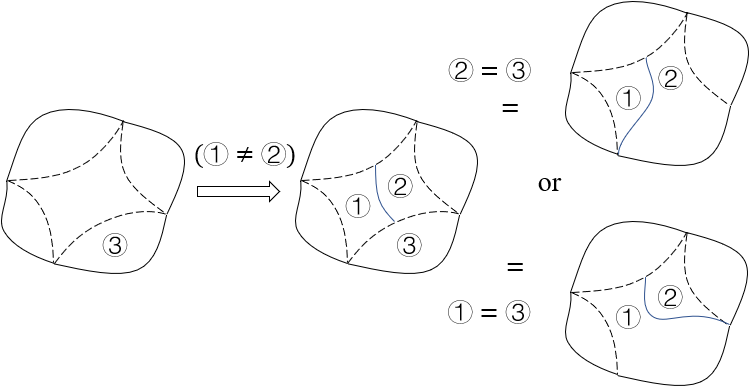
\includegraphics[width = 0.39\textwidth]{figures/TMech_simply_connected_example/equiv_cutting_path}\label{fig:from_endpoint}
}
\subfigure[Example shows that it is unnecessary to consider cutting paths that stretch across edges.]{
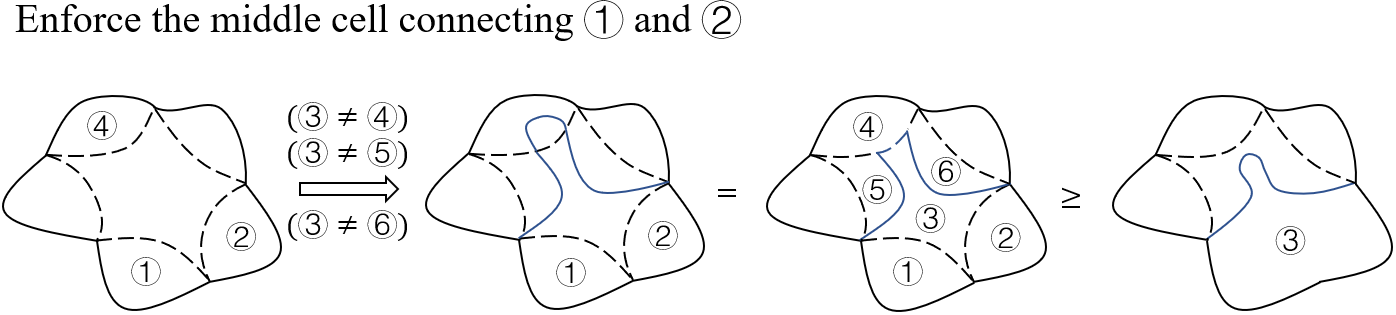
\includegraphics[width = 0.44\textwidth]{figures/TMech_simply_connected_example/equiv_cutting_path2}\label{fig:no_intersect}
}
\subfigure[Example shows that intersecting cutting paths can be discarded.]{
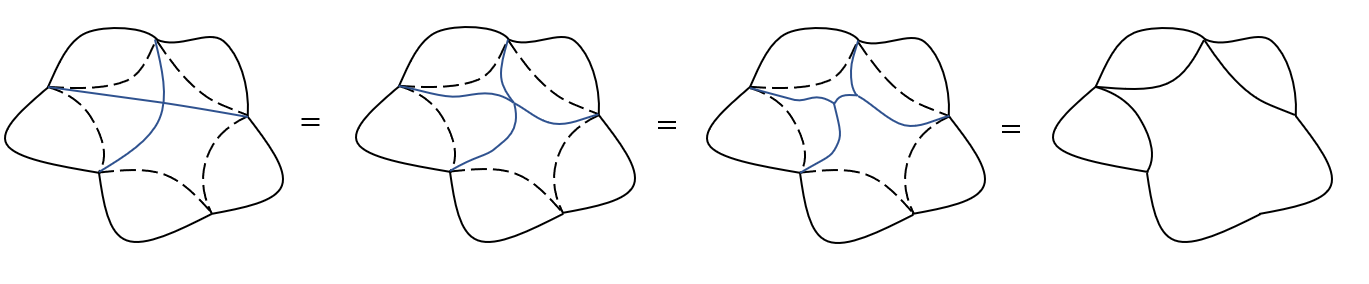
\includegraphics[width = 0.44\textwidth]{figures/TMech_simply_connected_example/equiv_cutting_path3}\label{fig:no_crossing}
}
\caption{Unnecessary or sub-optimal cell divisions cases can be safely discarded.}
\end{figure}

In earlier work~\cite{Yang2020Cellular}, the optimal SNCPP problem with least discontinuities was modelled as a 
topological graph with simply-connected cells, and the solution transformed into an optimal design strategy of a colour (configuration) scheme whereby the strategic placement of cutting paths would invariably 
lead to different colour vertices on both sides of a partition. An illustrative example is provided by Fig~\ref{fig:TMech}. 
In proving the finiteness of simply-connected cells, the following observations were proposed:
\begin{enumerate}
\item It is sufficient to consider cutting paths that start and end at the topological edge end-points. See Fig.\ref{fig:from_endpoint}. Let a cutting path divide the middle $4$-edge cell ending at an arbitrary point of the edge connecting to cell $3$, it implicitly specifies the subcell $1$ and $2$ to have different colours. If $1\neq 3$ and $2\neq 3$ then the division is trivial. However, whatever $1 = 3$ or $2 = 3$, we can continuous move the endpoint of the edge to the intersection of topological edges without breaking the connectivity of colours. Hence, for a complete solution it is sufficient to only consider cutting paths which start and end at the intersection of edges.
\item It is unnecessary to consider cutting paths that stretch across edges. See Fig.\ref{fig:no_intersect}. Because if a cutting path go across an edge, after we homotopically transform the cutting path back onto the edges, some sub-cells may be prevented from being coloured together, which leads to non-optimality, such as the cell $4$ and cell $5$ in this case. 
\item Intersecting cutting paths can be discarded. See Fig.\ref{fig:no_crossing}. The cutting paths can be always continuously transformed onto the edges, thus can be safely disregarded. 
\end{enumerate}

\begin{figure}[t]
\centering
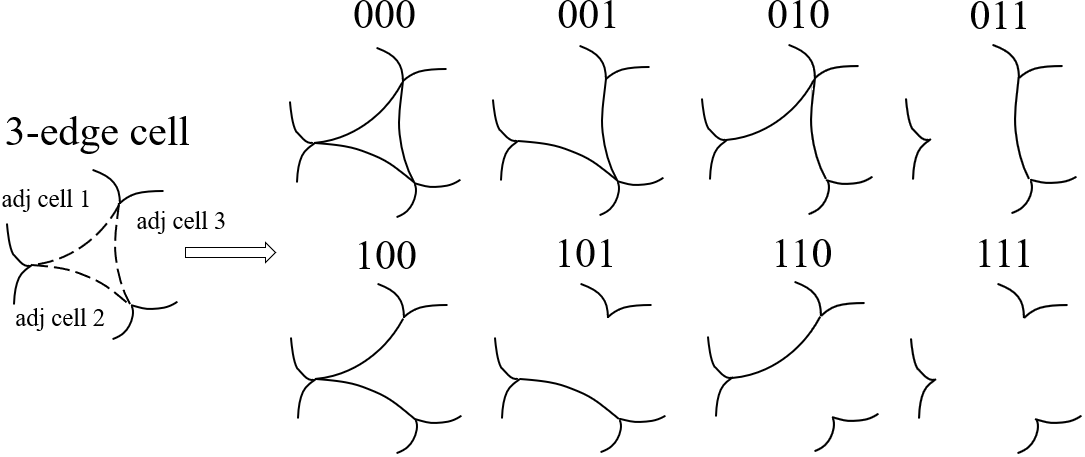
\includegraphics[width = 0.44\textwidth]{figures/TMech_simply_connected_example/cell3}
\caption{Possible divisions of a $3$-edge cell, as the most complex situation that need not further divisions. It can be observed how some of them are the same in terms of topological structure (e.g. $001, 010$ and $100$), or the division is impossible (e.g. $011$ is enforced, but cell $1$ and $2$ do not have the same colour), it is clearly already a finite problem, and the description of further simplifications is omitted for clarity and space constraints. }\label{fig:3cell}
\end{figure}

In solving the simply-connected cells, all different cellular decompositions of a simply-connected cell with $K$ topological edges are indexed by a binary number of length $K$ which represents the connectivity between this cell and its adjacent cells, $1$(connected, removing the edge), $0$(disconnected, keeping the edge). An illustration of a $3$-edge cell is shown in Fig.\ref{fig:3cell}. 
Instead of designing the cutting paths, we only need to specifying the connectivity (the binary number), then the corresponding topological cellular decomposition is unique. 
To solve a simply-connected cell with $K$ edges, the total number of different divisions $\Phi$ is bound by 
\begin{equation}
\label{equ_Psi}
\Phi(K) \leq 2^K
\end{equation}
where for simplicity we omit a constance of the exponential function corresponding to the number of possible colours to paint this cell. 
The cost of a (partly filled) graph is the number of colour segments in the current portion of the graph, i.e., $1$ colour equals to cost $ = 1$. The cost calculation is then described incrementally, whereby after a cell is solved, 
\begin{enumerate}
\item if its connectivity is all zero, then the cost will increase $1$ after freshly colouring this cell. 
\item if its connectivity has only one $1$ connection to an already solved cell, then the cost will remain unchanged, because the cell can be filled together with the connected adjacent cell. 
\item if its connectivity has $i$ 1s, there may exist multiple edges which connecte the same adjacent cell, as per the illustration in Fig.\ref{fig:cost}. In order to be consistent with the physical meaning of the cost, if these edges connect $j$ distinct solved cells, then the variation of cost is
\begin{equation}\label{equ_cost}
\Delta\mbox{cost} = 1-j
\end{equation}
\end{enumerate}
\begin{figure}[t]
\centering
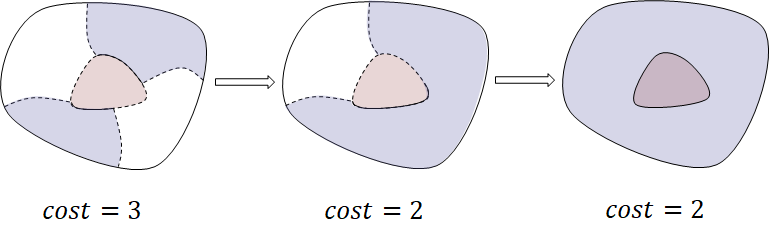
\includegraphics[width=0.44\textwidth]{figures/TMech_simply_connected_example/cost}
\caption{Cost variation calculation. 
Left: the right cell connects two distinct cells with same colour, so cost variation (\ref{equ_cost}) is $1-2 = -1$. Right: two edges connect with the same adjacent cell, cost variation (\ref{equ_cost}) is $1-1=0$.}\label{fig:cost}
\end{figure}

%<ty> I want the following part to appear in RSS21/TRO together with the instant solution of graph
\begin{comment}
\begin{color}{blue}
Another note is about the computing process. Although the algorithm is visually illustrated thorough this paper, the solving process can be purely algebraic. For example, let the cell $1$ have adjacent cells indexed by $2, 3, 4, 5, 6, 7, 8, 9$, then specifying connection between between $3$ and $7$ means the following separation and concatenation of the connectivity strings
\begin{equation}
\begin{aligned}
&\mbox{cell 1:}(x_2, x_3, x_4, x_5, x_6, x_7, x_8, x_9)\\
\Rightarrow&\left\{
\begin{aligned}
&\mbox{cell 1:} (x_2, 0_{10}, x_8, x_9), \mbox{color:}p_1\\
&\mbox{cell 10:} (0_{1}, x_3, 0_{11}, x_7), \mbox{color:}p_{10}\\
&\mbox{cell 11:} (0_{10}, x_4, x_5, x_6), \mbox{color:}p_{11}
\end{aligned}
\right.
\end{aligned}
\end{equation}
which means that the original cell $1$ is divided into three sub-cells, where the one connecting cell $2$ is still labeled as cell $1$, while other sub-cells are given new labels $10$ and $11$. The new number $0_{1}, 0_{10}, 0_{11}$ take the place of the corresponding sub-strings, which correspond to the cutting paths. 
If $x_2 = 1_2$ but $p_1\neq p_2$ then we get a contradiction and stop further searching process in this branch.
It is easy by inspection that after all $x$ and $p$ in the algebraic expression are determined, the group of numbers corresponds to a unique designing scheme of cutting paths. 
\end{color}
\end{comment}

In the following sections, a generalisation to genus-$n$ cells is derived.
\end{color}

\section{Solution of Genus-One Cells}
\label{section_genus_one}
\noindent
\indent
A cutting path connecting the inner part and the outer part of a genus-one cell will transform the cell into a 
simply-connected cell, proven to be finitely solvable. 
In this section we consider two cases: keeping the genus-one structure or transforming the genus-one cell into 
simply-connected sub-cells. In the former case, we prove that the inner part and the outer part can be seen as two independent problems. 
While in the later case, by efficiently discarding equivalent cellular decompositions, the number of possible subdivisions is proven to be finite, 
and all optimal solutions thus finitely solvable. An upper-bound on the complexity of solving a genus-one cell is also derived.  

For notation, a genus-one cell is denoted by $\Omega$, with its inner boundary and outer boundary denoted by $\omega$ and $\omega'$, 
respectively. The edges and cutting paths are denoted by $\alpha$. 

\subsection{Independence of Inner and Outer Parts}
\label{subsection_un_inner_cell}
\begin{figure}[t]
\centering
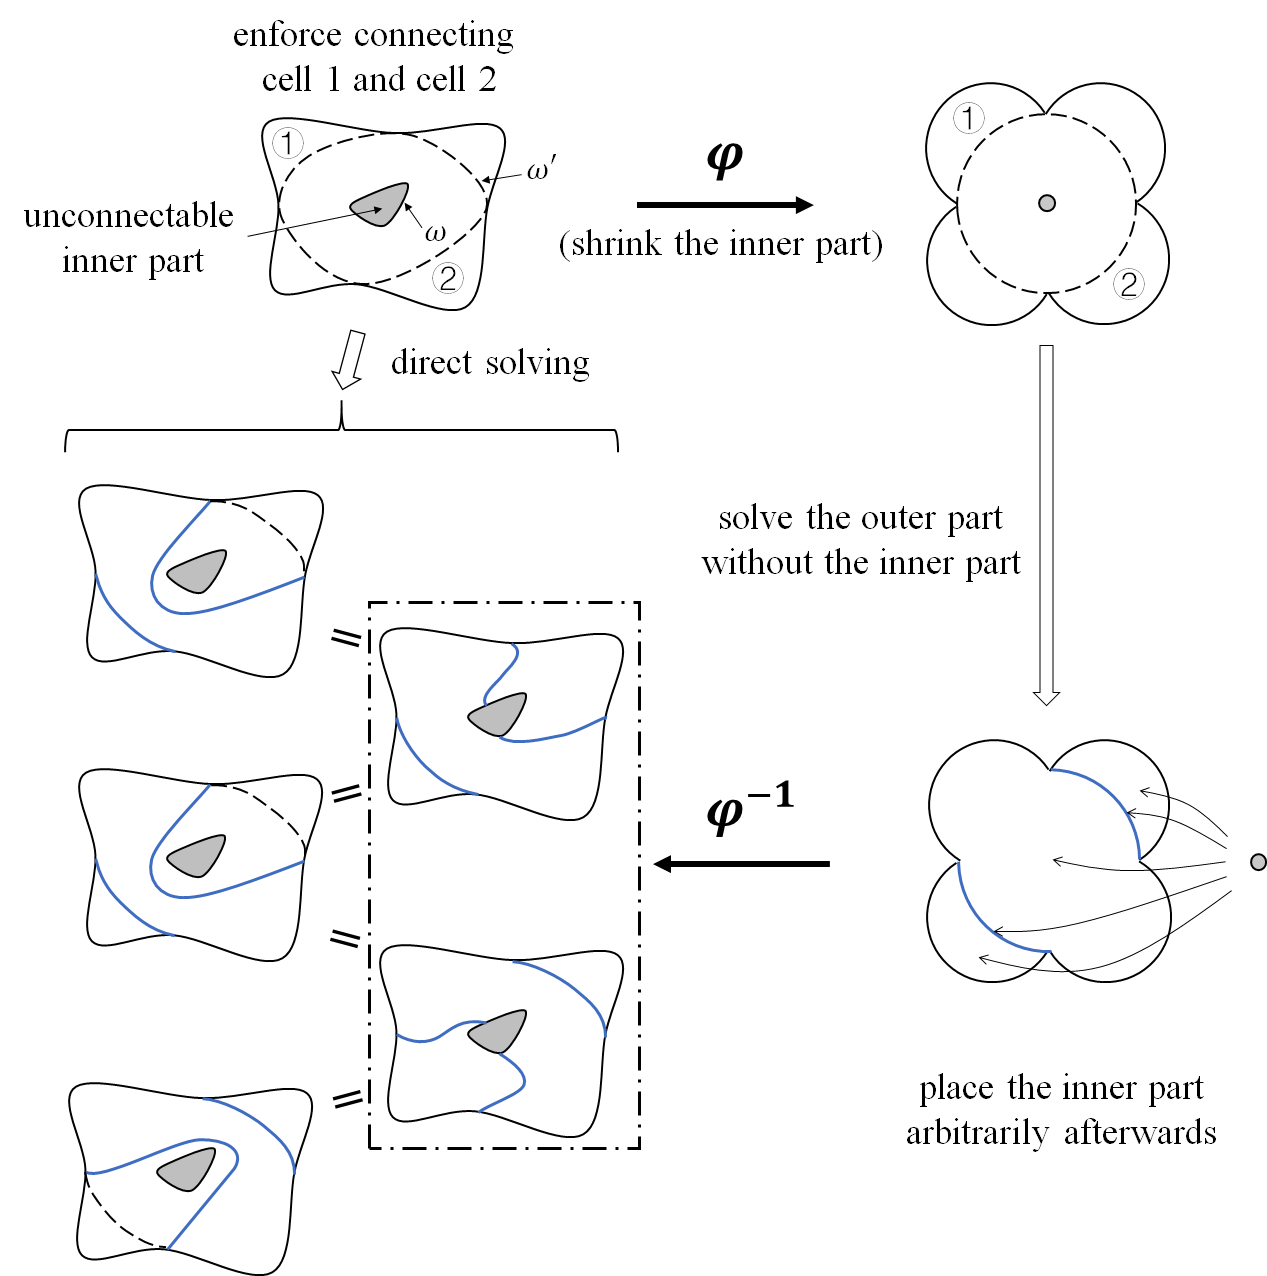
\includegraphics[width = 0.46\textwidth]{figures/RSS_related_figures/proof/fig_physical_hole_6}
\caption{Example showing that the unconnectable inner part (marked in grey) is negligible when solving the outer part. 
In this simple example the direct solutions are straightforward, and they are equivalent to first solving the outer part without the inner part, 
and then arbitrarily replacing back the inner part. It can also be observed how the inner part can be placed ``on'' a cutting path 
(dashed block), yet there is no need not consider these cases since they are effectively equivalent to the three divisions shown on the left under a continuous cutting path transformation. 
\textcolor{blue}{In other words, the inner part is a $1$-edge cell, thus we only to consider whether keep the edge or remove the edge.}  
}
 \label{fig_physical_hole}
\end{figure}

The situation when inner part and the outer part of $\Omega$ are not connected arises when the inner part is a physical hole, 
the inner part can only be covered with a totally different colour from that of the outer part, or when all the edges in $\omega$ must be retained. 
In these cases, first we prove that the inner part of $\Omega$ is negligible when solving the outer part. 
To show this equivalence, let $\varphi$ be a homeomorphic mapping 
from $\Omega$ to the standard unit disk $D$, with its boundaries mapped onto concentric circles, 
\begin{equation}
\varphi: \Omega\rightarrow D, \omega'\mapsto \mathbb{S}^1(1), \omega\mapsto \mathbb{S}^1(\delta), \delta\rightarrow 0^+
\end{equation}
then the inner part becomes an infinitesimal open neighbourhood of the origin. See Fig.~\ref{fig_physical_hole} for illustration. 
Let a cutting path of $D$, $\varphi(\beta)$, start and end at $\varphi(\omega')$, then it must be one of the following two cases:
\begin{equation}
\label{equ_nocross}
\begin{aligned}
&(0, 0)\notin \varphi(\beta)\\
\Rightarrow &\exists \epsilon > 0, B(0, \epsilon) \cap \varphi(\beta) = \varnothing\\
\Rightarrow &\mbox{let } \delta < \epsilon, \mbox{ then } \varphi(\omega)\cap \varphi(\beta) = \varnothing\\
\Rightarrow & \omega\cap \beta = \varnothing
\end{aligned}
\end{equation}
where $B(x, r)$ is an open ball centering at $x$ with radius $r>0$, or 
\begin{equation}
\label{equ_cross}
\begin{aligned}
&(0, 0)\in \varphi(\beta)\\
\Rightarrow &\varphi(\omega)\cap \varphi(\beta) \neq \varnothing, \forall \delta\\
\Rightarrow & \omega\cap \beta \neq \varnothing
\end{aligned}
\end{equation}
All the different topological divisions described by ~(\ref{equ_nocross}) and~(\ref{equ_cross}) correspond to those listed in Fig.~\ref{fig_physical_hole}.
\begin{color}{blue}
On a side note, it can be seen in Fig.\ref{fig_physical_hole} that a $1$-edge cell should not be connected by any cutting path. To instead, we only need to consider its existence. 
\end{color}
 
Next, we prove the inverse claim that the outer part of $\Omega$ is negligible when solving the inner part.  
Let a sphere with radius $r$ stand within the inner part (anywhere is applicable but a place within the inner part will simplify the
 description), and $\psi$ be the stereographic projection~\cite{coxeter1961introduction}
\begin{equation}
\begin{aligned}
\psi: \mathbb{R}^2&\rightarrow \mathbb{S}^2\backslash \mathfrak{n}\\
(x, y, 0)&\mapsto (\frac{4r^2x}{x^2 + y^2 + 4r^2}, \frac{4r^2y}{x^2 + y^2 + 4r^2}, \frac{2r(x^2 + y^2)}{x^2 + y^2 + 4r^2})
\end{aligned}
\end{equation}
\begin{figure}[t]
\centering
\subfigure[]{ 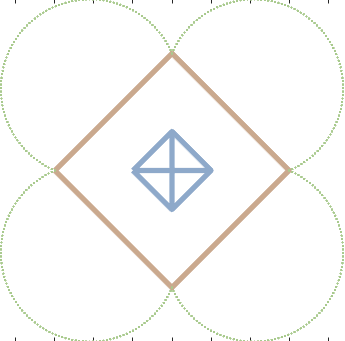
\includegraphics[width = 0.11\textwidth]{figures/RSS_related_figures/proof/fig_stereo_1}}
\subfigure[]{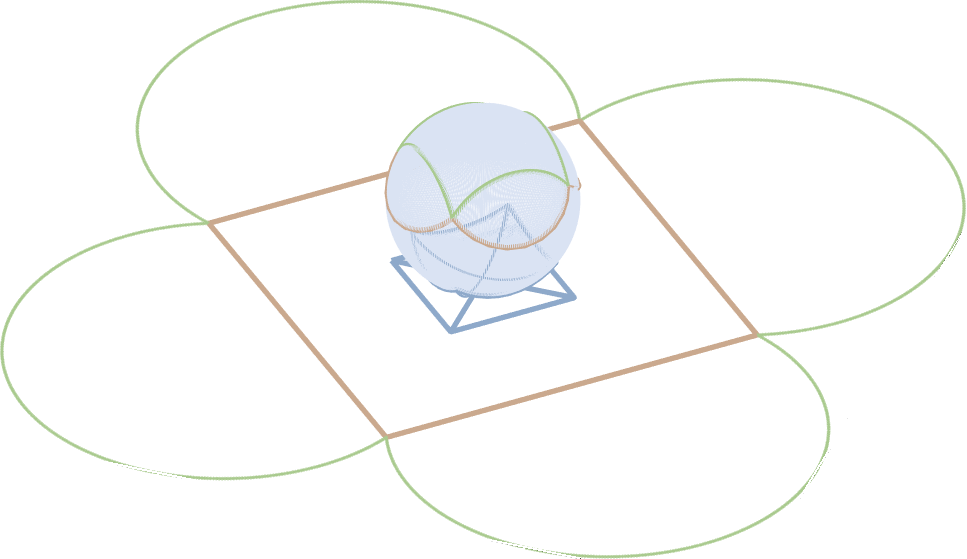
\includegraphics[width = 0.13\textwidth]{figures/RSS_related_figures/proof/fig_stereo_2}}
\subfigure[]{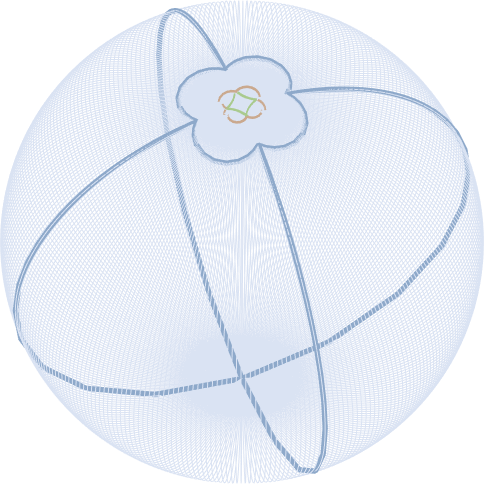
\includegraphics[width = 0.11\textwidth]{figures/RSS_related_figures/proof/fig_stereo_3}}
\caption{ (a) Topological graph with a genus-one cell enforced to be kept (the area between concentric squares). 
(b) A stereographics projection using a sphere lying within the inner boundary. 
(c) Let the radius of the sphere be small enough, then the inner part of graph and the outer part interchange 
near the north pole of the sphere. }
\label{fig_stereographic_projection}
\end{figure}
where $\mathfrak{n}$ denotes the arctic point. See Fig.~\ref{fig_stereographic_projection} for illustration. Since $\psi$ is homeomorphic, 
the transformed graph on the sphere is equivalent to the original graph.  $\psi$ maps the outer part (including the uncoverable ambient 
space) to a neighbourhood of the arctic point (the $\infty$ point to the arctic point), and the inner part to a neighbourhood of the antarctic point. 
Let $r\rightarrow 0$, the roles of the inner part and the outer part interchange near the arctic point. 
Recalling the observation of the negligibility of the inner part, we finish the proof.

In summary, when the inner part and the outer part are not connected, they can be solved independently and their results can be merged directly.

\subsection{Negligibility of Cyclic and Single Cutting Paths}
Cutting paths connecting $\omega$ and $\omega'$ can be classified based on their number of cycles, as depicted by Fig.~\ref{fig_cycle}. 
However, Fig.~\ref{fig_no_cyclic_cutting_path} shows that all cyclic cutting paths have the same topological function as the acyclic one, 
thus can be safely disregarded. 
Note however that unlike the case for other equivalences, the physical cellular decomposition using the cyclic cutting paths cannot be generated through continuously modifying the position of the acyclic ones. Here the equivalence means that only the acyclic situations require explicit consideration. Once an acyclic solution is optimal, all equivalent solutions using the cyclic cutting paths are all optimal and automatically considered. 
%\begin{figure}[t]
%\centering
%\includegraphics[width = 0.44\textwidth]{figures/proof/fig_cycle}
%\caption{The classification of the cutting paths. One acyclic cutting path corresponds to a family of cyclic cutting paths that share the same start point and end point but go through different cycles.}\label{fig_cycle}
%\end{figure}
%
%\begin{figure}[t]
%\centering
%\includegraphics[width = 0.48\textwidth]{figures/proof/fig_no_cyclic_cutting_path}
%\caption{The cyclic cutting paths can be safely disregarded because they serve as the same function as the acyclic cutting paths in the sense of topological structure. The grey cell is the created sub-cell (here only one sub-cell is created). 
%The below three figures show a continuous transformation (rotation) from the $1$-cycle division and $0$-cycle division. The result is easy to generalize to $n$-cycles cases. }\label{fig_no_cyclic_cutting_path}
%\end{figure}
\begin{figure}[t]
\centering
\subfigure[Each acyclic cutting path corresponds to a family of cyclic cutting paths that go through different cycles.]{
	\includegraphics[width = 0.44\textwidth]{figures/RSS_related_figures/proof/fig_cycle}
	\label{fig_cycle}}
\subfigure[Continuous transformation between the $0$-cycle division and $1$-cycle division, with similar results for the $n$-cycles case.]{
	\includegraphics[width = 0.44\textwidth]{figures/RSS_related_figures/proof/fig_no_cyclic_cutting_path}
	\label{fig_no_cyclic_cutting_path}}
\caption{Examples of negligible cutting paths.}
\end{figure}


%\begin{figure}[t]
%\centering
%\subfigure[]{
%\includegraphics[width=0.14\textwidth]{figures/proof/fig_one_cutting_path_1}
%}
%\subfigure[]{
%\includegraphics[width=0.14\textwidth]{figures/proof/fig_one_cutting_path_2}
%}
%\subfigure[]{
%\includegraphics[width=0.14\textwidth]{figures/proof/fig_one_cutting_path_3}\label{fig_one_cutting_path:c}
%}
%\caption{(a) One cutting path can connect two inner cells. (b) One cutting path can connect two outer cells. (c) But one cutting path cannot transform the genus-one cell into simply-connected cells, because the two sides of the cutting path are the same cell, which are impossible to have different colours. }\label{fig_one_cutting_path}
%\end{figure}

%Next, see a counter-example in Fig. \ref{fig_one_cutting_path:c}, where a single cutting path can only lead to contradiction. 
Next, we observe that if there is only one cutting path that connects $\omega$ and $\omega'$, then $\Omega$ is transformed into a 
single simply-connected sub-cell. However, this becomes a contradiction since both sides of the cutting paths are effectively the same cell, 
thus impossible to have different colors. It is therefore apparent that it is not the cutting path but the connected area what determines 
the division of $\Omega$. More precisely, an area connecting the inner part and the outer part of $\Omega$. 
This observation motivates us to directly consider the connectivities between cells. Based on the remarks in 
Section~\ref{section_simply_connected}, we only need to judge whether keeping or removing each edge. 
Let the indices of $J$ edges in $\omega$ and $K$ edges in $\omega'$ be (in cyclic order) 
\begin{equation}\label{equ_omega}
\omega = (\alpha_1, \cdots, \alpha_J)
\end{equation}
\begin{equation}\label{equ_omega_prime}
\omega' = (\alpha'_1, \cdots, \alpha'_K).
\end{equation}
Arbitrarily choosing some edges in $\omega$ and $\omega'$ to generate a connectivity, like
\begin{equation}\label{equ_example_division}
(\{\alpha_{i_1}, \cdots, \alpha_{i_r}\}, \{\alpha'_{j_1}, \cdots, \alpha'_{j_s}\} ), 1\leq r\leq J, 1\leq s\leq K
\end{equation}
where $\{\}$ means the order has no meaning, leads to valid divisions of the $\Omega$. An example is shown in 
Fig.\ref{fig_not_same_cutting_path}, where it is apparent that results are not unique. The finiteness of this approach is discussed next. 


\subsection{Assignment of Cutting Paths Based on Connectivity}
\label{subsection_arbitrary_assignment}
Extracting all combinations from (\ref{equ_example_division}) does not necessarily mean listing all different divisions. 
In Fig. \ref{fig_not_same_cutting_path}, various divisions are created from the same connectivity. 
%Unlike the simply-connected case, the specified connectivity of a genus-one cell does not determine a unique structure of the cutting paths. For example, in Fig. \ref{fig_not_same_cutting_path}, different divisions are given based on a same connectivity. 
In order to address this issue, the whole division of $\Omega$ is regarded as a two-stage process, first transforming into simply-connected sub-cells and then undertaking further divisions in these sub-cells. 
We prove that in the first stage, only two cutting paths are required which connect $\omega$ and $\omega'$. 

First, all cutting paths that do not connect $\omega$ and $\omega'$ do not appear in the first stage, because they can be seen as further divisions in the generated sub-cells. Refer to Fig.~\ref{fig_equivalence} for an illustration of this phenomenon. 
%Hence, only those cutting paths that connect both $\omega$ and $\omega'$ need further discussion.
Then, let there be three cutting paths that connect $\omega$ and $\omega'$, then $\Omega$ is divided into three simply-connected sub-cells. However, the resulting topological structure is equivalent to $\Omega$ being firstly divided into two sub-cells, then another cutting path creating further divisions iteratively. Hence, there need to be at most two cutting paths in the first-stage.  

In summary, let~$\omega$ and~$\omega'$ be defined by~(\ref{equ_omega}) and~(\ref{equ_omega_prime}), during the first stage a continuous 
subset is identified in~$\omega$, and another one in~$\omega'$. The total number of different divisions is the number of different choices of these continuous subsets. To relieve the problem of the cyclic choices, we enforce the sub-cell $1$ be the one containing $\alpha_1$. 
So all choices in $\omega$ are described by
\begin{equation}\label{equ_all_omega}
\left\{
\begin{aligned}
&\{\alpha_1\}\ (1\mbox{ element})\\
&\{\alpha_1, \alpha_2\}, \{\alpha_J, \alpha_1\}\ (2\mbox{ elements})\\
&\{\alpha_1, \alpha_2, \alpha_3\}, \{\alpha_J, \alpha_1, \alpha_2\}, \{\alpha_{J-1}, \alpha_J, \alpha_1\}\ (3\mbox{ elements})\\
&\cdots\\
&\{\alpha_1, \cdots, \alpha_{J-1}\}, \cdots, \{\alpha_3, \cdots, \alpha_J, \alpha_1\}\ (J-1\mbox{ elements})
\end{aligned}
\right.
\end{equation}
Likewise, all choices in $\omega'$ are given by
\begin{equation}\label{equ_all_omega_prime}
\left\{
\begin{aligned}
&\{\alpha_1'\}, \{\alpha_2'\}, \cdots, \{\alpha_K'\}\ (K\mbox{ elements})\\
&\{\alpha_1', \alpha_2'\}, \cdots, \{\alpha_K', \alpha_1'\}\ (K\mbox{ elements})\\
&\{\alpha_1', \alpha_2', \alpha_3'\}, \cdots, \{\alpha_{K}', \alpha_1', \alpha_2'\}\ (K\mbox{ elements})\\
&\cdots\\
&\begin{aligned}
 \{\alpha_1', \cdots, \alpha_{K-1}'\}, &\{\alpha_K', \alpha_1', \cdots, \alpha_{K-2}'\},\\
 &\cdots, \{\alpha_2', \cdots, \alpha_K'\}
\end{aligned}
\ (K\mbox{ elements})
\end{aligned}
\right.
\end{equation}
%So all choices in $\omega$ and $\omega'$ are
%\begin{align}
%&\left\{
%\begin{aligned}\label{equ_all_omega}
%&\{\alpha_1\}\\
%&\{\alpha_1, \alpha_2\}, \{\alpha_J, \alpha_1\}\\
%&\{\alpha_1, \alpha_2, \alpha_3\}, \{\alpha_J, \alpha_1, \alpha_2\}, \{\alpha_{J-1}, \alpha_J, \alpha_1\}\\
%&\cdots\\
%&\{\alpha_1, \cdots, \alpha_{J-1}\}, \cdots, \{\alpha_3, \cdots, \alpha_J, \alpha_1\}
%\end{aligned}
%\right.\\
%%\end{equation}
%%and all choices in $\omega'$ are
%%\begin{equation}
%&\left\{
%\begin{aligned}\label{equ_all_omega_prime}
%&\{\alpha_1'\}, \{\alpha_2'\}, \cdots, \{\alpha_K'\}\\
%&\{\alpha_1', \alpha_2'\}, \cdots, \{\alpha_K', \alpha_1'\}\\
%&\{\alpha_1', \alpha_2', \alpha_3'\}, \cdots, \{\alpha_{K}', \alpha_1', \alpha_2'\}\\
%&\cdots\\
%&\{\alpha_1', \cdots, \alpha_{K-1}'\}, \{\alpha_K', \alpha_1', \cdots, \alpha_{K-2}'\}, \cdots, \{\alpha_2', \cdots, \alpha_K'\}
%\end{aligned}
%\right.
%\end{align}

\begin{figure}[t]
\centering
\includegraphics[width = 0.44\textwidth]{figures/RSS_related_figures/proof/fig_only_one_division_3}
\caption{In this example, cells $1$, $3$, $7$ and $10$ are enforced to be connected.
The four distinct divisions shown on the right are all valid, exemplifying the non-uniqueness of the subdivision problem.
%We can see at the right side there are four different divisions having the same function. 
}\label{fig_not_same_cutting_path}
\end{figure}

\begin{figure}[t]
\centering
\subfigure[Illustration of cutting paths that start and end at the same boundary, which can be seen as further divisions (in sub-cell $2$, shown in red).]{
	\includegraphics[width=0.45\textwidth]{figures/RSS_related_figures/proof/fig_equivalence_1}}
\subfigure[Example shows that the third (and later) cutting paths connecting $\omega$ and $\omega'$ can be seen as further divisions (in sub-cell $2$, shown in red).]{
	\includegraphics[width=0.45\textwidth]{figures/RSS_related_figures/proof/fig_equivalence_2}}
\caption{The placement of cutting paths can be seen as a two-stage processes: First we only place two cutting paths that connect the inner boundary and the outer boundary, and then place all other cutting paths within the simply-connected sub-cells, seen as further divisions of the sub-cells.}
\label{fig_equivalence}
\end{figure}

\subsection{Complexity Analysis}\label{subsection_genus_one_complexity}
When $\omega$ and $\omega'$ are connected, there are $r$ methods to choose $r$ continuous edges in $\omega$ containing $\alpha_1$, i.e., 
\begin{equation}
\{\alpha_{J-r+1}, \cdots, \alpha_J, \alpha_1\}, \cdots, \{\alpha_1, \cdots, \alpha_r\}
\end{equation}
and $K$ methods to choose $s$ continuous edges in $\omega'$. Summarising all possible $r$ and $s$ we get
\begin{equation}\label{equ_Psi_1}
\Psi(J, K) = \sum\limits_{r = 1}^{J-1}\sum\limits_{s = 1}^{K-1} rK\Phi(r+s)\Phi(J+K -r-s)
\end{equation}
with $\Phi$ defined by~(\ref{equ_Psi}). 
\begin{color}{blue}
This is the complexity for the genus-one cell under the assumption that it is divided into simply-connected sub-cells. 
\end{color}
Moreover, from Section \ref{subsection_un_inner_cell}, the number of different divisions keeping a genus-one structure is 
\begin{equation}\label{equ_Phi_0}
\Phi_0(J, K) = \Phi(J) + \Phi(K) = 2^J + 2^K
\end{equation}
\begin{color}{blue}
where the subscript $0$ means that the ring structure of $\omega$ to be kept in the final cellular decomposition. 
\end{color}
Hence the total number of different divisions for a genus-one cell with $J$ edges in the inner boundary and $K$ edges in the outer boundary is given by
\begin{equation}
\Phi(J, K) = \Phi_0(J, K) + \Psi(J, K)
\end{equation}

\section{Solution of Large Genus Cells}
\label{section_large_genus}
There are $n$ inner boundaries in a genus-$n$ cell. Taking the outer boundary into consideration, there are $C_{n+1}^2$ 
possible ``starting-  ending-point" pairs for the possible cutting paths, which are impractical to enumerate and deal with. 
Hence, a multi-stage iterative strategy is once again proposed to transform a genus-$n$ cell into sub-cells with genus no more than $n-1$. 

\subsection{Genus-Two Cell Case}
Following a deduction process similar to the one in Section~\ref{subsection_un_inner_cell}, the ensuing equivalence states arise:
\begin{enumerate}
\item The disconnected inner part can be safely discarded and the remaining becomes a genus-one cell which has been proved solvable. 
After solving both the genus-one cell and the unconnectable part independently, we can arbitrarily place the resulting division of the 
disconnected inner part in the result of the genus-one cell. 
\item When both inner parts are unconnectable, the genus-two cell can be seen as three simply-connected parts. And the solution comes from the arbitrary placements of the solution of the inner parts in the result of the outer part. 
\end{enumerate}

For a genus-$n$ cell, if any of its inner part is disconnected, the genus-$n$ problem becomes a genus-$(n-1)$ problem which is proven solvable under induction. Hence, in this section the focus is on the case when all boundaries are forced to be connected. 

%We introduce the notations. 
Following the notation of a genus-one cell, a genus-two cell is also denoted by $\Omega$, with its outer boundary described by 
\begin{equation}
\label{equ_omega_genus_two}
\omega = (\alpha_1, \cdots, \alpha_K)
\end{equation}
and the inner boundaries given by
\begin{equation}
\label{equ_omega_genus_two_1}
\omega^1 = (\alpha^1_1, \cdots, \alpha^1_{J_1})
\end{equation}
\begin{equation}
\label{equ_omega_genus_two_2}
\omega^2 = (\alpha^2_1, \cdots, \alpha^2_{J_2})
\end{equation}
where $\alpha_*^*$ are the edges in each boundary listed in cyclic order. 

\begin{figure*}[t]
\centering
\includegraphics[width = 0.96\textwidth]{figures/RSS_related_figures/proof/fig_no_on_cutting_path}
\caption{Example showing that at each stage, cost-wise it is unnecessary to place the second inner part on the 
cutting paths created earlier (in blue).}
\label{fig_no_on_cutting_path}
\end{figure*}

Similar to the process illustrated in Section~\ref{section_genus_one}, we regard the whole division of $\Omega$ as a three-stage process. 
In the first stage, we consider the generation of the cutting paths connecting $\omega$ and $\omega^1$. 
As per the discussion in Section~\ref{subsection_arbitrary_assignment}, at this point there are only two cutting paths, generating two sub-cells. 
In the second stage, we place $\omega^2$ in each of the sub-cells. 
In either case, the sub-cell containing $\omega^2$ becomes a genus-one cell. 
Then it can be solved through further division. 
After creating other two cutting paths, $\Omega$ is transformed into three simply-connected sub-cells. 
In the third stage, all other cutting paths are created. 

\subsection{Negligibility of Putting Inner Part on the Cutting Paths}
A special case may first appear to arise when placing $\omega^2$ within each sub-cell generated in the first stage intersecting 
the actual cutting path created (seen in blue in Fig.~\ref{fig_no_on_cutting_path}) 
%unnecessary to consider the place intersecting the generated cutting paths created in the first stage. 
Yet this is a case that requires no consideration given the equivalence shown in the same Figure. 
Since $\omega^2$ is not assumed unconnectable, if a cutting path lies on the existing topological edges, it prevents further connections
(such as the one shown in red in Fig.~\ref{fig_no_on_cutting_path}), leading to higher cost. 
Recalling the result from Section~\ref{subsection_arbitrary_assignment}, there are only two cutting paths dividing $\Omega$ into two parts, so there are exactly two different places to put $\omega^2$, i.e., in either sub-cell created in the first stage. 

\subsection{Complexity Analysis of Solving Genus-Two Cells}
\label{subsection_genus_two_complexity}
When $\omega^1$ and $\omega^2$ are both disconnected, similar to~(\ref{equ_Phi_0}), 
\textcolor{blue}{two $0$s are used as subscripts to denote this case, }
we have
\begin{equation}\label{equ_Phi_00}
\Phi_{00}(J_1, J_2, K) = 2^{J_1} +2^{J_2} + 2^K
\end{equation}
If $\omega$ and $\omega^1$ are connected, but $\omega^2$ is disconnected, 
\begin{equation}\label{equ_Phi_10}
\Phi_{10}(J_1, J_2, K) = \Psi(J_1, K)+\Phi(J_2)
\end{equation}
exchanging the role of $\omega^1$ and $\omega^2$, 
\begin{equation}\label{equ_Phi_01}
\Phi_{01}(J_1, J_2, K) = \Psi(J_2, K) + \Phi(J_1)
\end{equation}

When both $\omega^1$ and $\omega^2$ are connected, the complexity can be calculated by considering $\omega^2$ being placed in 
different sub-cells separately. Using $\Xi_1$ for the situations that $\omega^2$ is placed in sub-cell $1$, 
and $\Xi_0$ for sub-cell $2$ give rise to
%Assume that in the first stage, $r_1$ edges from $\omega^1$ and $s$ edges from $\omega$ are chosed to form sub-cell $1$, then the number of divisions in the second stage is
\begin{equation}
\Xi_{1}(J_2; r_1, J_1, s, K) = \Psi(J_2, r_1+s)\Phi(J_1+K-r_1-s)
\end{equation}
\begin{equation}
\Xi_{0}(J_2; r_1, J_1, s, K) = \Phi(r_1+s)\Psi(J_2, J_1+K-r_1-s)
\end{equation}
%\begin{equation}
%\Phi_1(J_2, r_1+s)2^{J+K-r_1-s} + 2^{r_1+s}\Phi_1(J_2, J+K - r_1 - s)
%\end{equation}
Going through all possible $r_1$ and $s$, we have 
\begin{equation}\label{equ_Phi_11}
\begin{aligned}
\Psi(J_1, &J_2, K) = \sum\limits_{r_1 = 1}^{J_1-1}\sum\limits_{s = 1}^{K-1}\\
&r_1K\left[\Xi_1\left(J_2; r_1, J_1, s, K\right) + \Xi_0\left(J_2; r_1, J_1, s, K\right)\right]
\end{aligned}
\end{equation} 
Summarising (\ref{equ_Phi_00}), (\ref{equ_Phi_10}), (\ref{equ_Phi_01}) and (\ref{equ_Phi_11}), the final result is compouned by
\begin{equation}
\begin{aligned}
\Phi(J_1, J_2, K) =& \Phi_{00}(J_1, J_2, K) + \Phi_{01}(J_1, J_2, K)\\
& + \Phi_{10}(J_1, J_2, K) + \Psi(J_1, J_2, K)
\end{aligned}
\end{equation}

\subsection{Genus-$n$ Cell Case}
Let $\Omega$ be a genus-$n$ cell, with its outer boundary denoted by $\omega$ and inner boundaries denoted by $\omega^1, \cdots, \omega^n$. The edges and their order in each boundary are given by (\ref{equ_omega_genus_two}) and 
\begin{equation}\label{equ_inner_boundaries}
\omega^i = (\alpha^i_1, \cdots, \alpha^i_{J_i}), \forall i = 1, \cdots, n
\end{equation}
Again, we assume that all $\omega^i$ must be connected, or else the disconnected inner parts can be safely discarded, then the genus-$n$ problem becomes a lower-genus problem. 

Similar to our discussion of the genus-two cell, the whole division of a genus-$n$ cell can be seen as an $(n+1)$-stage process. 
At each stage, $\omega^i$ is added to one of the sub-cells, transforming it into a genus-one sub-cell. Then, exactly two new cutting paths are required to transform this sub-cell again into two simply-connected sub-cells. 
%After the $i$-th stage, the original genus-$n$ cell has been divided into $(i+1)$ simply-connected sub-cells, so there are $(i+1)$ possible places to put $\omega^{i+1}$. 
After $n$ stages, $\Omega$ becomes an enssemble of simply-connected sub-cells. The process is illustrated 
by Fig.~\ref{fig_iterative_process}. 

\begin{figure*}[t]
\centering
\includegraphics[width=0.96\textwidth]{figures/RSS_related_figures/proof/fig_iterative_process_2}
\caption{Iterative transformation process of the genus-$n$ case.}%This example shows the process of each stage with an assigned connectivity.}
\label{fig_iterative_process}
\end{figure*}

\subsection{Complexity Analysis of Solving Genus-$n$ Cells}
The number of different divisions can be classified based on whether each inner part is connected. 
For a genus-$n$ cell, define the subscript $T_n$ as a binary string with length $n$, where the digit sum of $T_n$ is $N(T_n)$. 
For example, $N(T_n) = 0$ represents the case that none of the inner boundaries are connected. In this case, 
%If none of the inner boundaries is connected, then $N(T_n)$ = 0
\begin{equation}\label{equ_n_0}
\Phi_{0	\cdots 0}(J_1, \cdots, J_n, K) = 2^{J_1} + \cdots + 2^{J_n} + 2^K
\end{equation} 
If $N(T_n) = 1$, e.g., $\omega$ and $\omega^1$ are connected - and a genus-$(n-1)$ structure is kept after the whole division -  the number of divisions are
%If $\omega^1$ and $\omega$ are connected (thus a genus-$(n-1)$ structure is kept after the whole division process),then ${\rm abs} N$ = 1 the number of different divisions is
\begin{equation}\label{equ_n_1}
\Phi_{1 0 \cdots 0}(J_1, \cdots, J_n, K) = \Psi(J_1, K) + 2^{J_2} + \cdots + 2^{J_n}
\end{equation}
There are $(C_n^1-1)$ terms with $N(T_n)=1$, e.g., $\Phi_{010\cdots 0}$ to $\Phi_{0\cdots 01}$, that can be calculated through exchanging the indices.
Similarily, an example for $N(T_n) = 2$ can be given by 
\begin{equation}\label{equ_n_2}
\Phi_{110\cdots0}(J_1, \cdots, J_n, K) = \Psi(J_1, J_2, K) + 2^{J_3} + \cdots + 2^{J_n}
\end{equation}
and $(C_n^2-1)$ terms can be calculated through exchanging the indices, 
$$\cdots $$
\begin{equation}\label{equ_n_n-1}
\Phi_{1\cdots 10}(J_1, \cdots, J_n, K) = \Psi(J_1, \cdots, J_{n-1}, K) + 2^{J_n}
\end{equation}
with other $(C_n^{n-1}-1)$ similar terms satisfying $N(T_n) = n-1$.

By induction, all the above mentioned terms can be calculated except for the one satisfying $N(T_n) = n$. %with all $1$s in the subscripts. 
After the first stage, we can choose which sub-cell each $\omega^i, i = 2, \cdots, n$ will eventually lie in, and $\Xi_{T_{n-1}}$ are used to consider each situation, with the $i$-th binary digit in $T_{n-1}$ representing that $\omega^i$ lies in sub-cell $1$ or sub-cell $2$. % is $0$ or $1$
Let $Q(T, i)$ be the value of the $i$-th digit in $T$,  
\begin{equation}
Q(T, i) = \frac{T}{2^{n-i}}\mbox{ mod } 2
\end{equation}
then
\begin{equation}\label{equ_Xi_n}
\begin{aligned}
&\Xi_{T_{n-1}}(J_2, \cdots, J_n; r_1, J, s, K) \\
=&\, \Psi(J_{i_2}, \cdots, J_{i_l}, r_1+s)\Psi(J_{i_{l+1}}, \cdots, J_{i_n}, J+K-r_1-s)
\end{aligned}
\end{equation}
where $i_2, \cdots, i_n$ are specified by
\begin{equation}
\left\{
\begin{aligned}
&Q(T_{n-1}, i_j) = 1, &j = 2, \cdots, l\\
&Q(T_{n-1}, i_j) = 0, &j = l+1, \cdots, n.
\end{aligned}
\right.
\end{equation}

It is easy to see that the order of $J_{i_*}$ does not effect the result in (\ref{equ_Xi_n}). So
\begin{equation}\label{equ_n_n}
\begin{aligned}
\Psi(J_1, \cdots, &J_n, K) = \sum\limits_{r_1 = 1}^{J_1 - 1} \sum\limits_{s = 1}^{K-1}\\
&\left(r_1K \sum\limits_{T_{n-1} = 0	}^{2^{n-1}-1}\Xi_{T_{n-1}}(J_2, \cdots, J_n; r_1, J, s, K) \right)
\end{aligned}
\end{equation}
Summarising the results from (\ref{equ_n_0}), (\ref{equ_n_1}), (\ref{equ_n_2}), (\ref{equ_n_n-1}), (\ref{equ_n_n}), 
%In summary, let $T$ be a binarial number of length $n$,
\begin{equation}
\begin{aligned}
\Phi(J_1, \cdots, J_n, K) = &\sum\limits_{T_n = 0}^{2^n-2}\Phi_{T_n}(J_1, \cdots, J_n, K)\\
& + \Psi(J_1, \cdots, J_n, K)
\end{aligned}
\end{equation}













To help the reader better understand the above formulae, we append a table of symbols and their physical meaning in Table \ref{table:symbols}.

\begin{table*}[h]
\small\sf\centering
\caption{The notation used in this paper. Some symbols have multiple meanings and their context must be used to disambiguate them. $i, j, k, l, n, r, s, \lambda$ are sometimes used for indexing without listing below.}\label{table:symbols}
\begin{tabular}{>{\bfseries}ll}
\toprule
\normalfont{Symbols}   &    Physical Meaning   \\
\midrule
%$A_m$ & A homogeneous open region containing point $m$ on the surface\\
$B(x, \epsilon)$ & An open ball with radius $\epsilon$ centering $x$\\
$\bar{\mathscr{C}}, \mathscr{C}$ & The manipulator configuration space, the set of all valid configurations\\
$c, c_i, i\in \mathbb{N}$ & A valid configuration\\ 
$c_{mi}, i\in \mathbb{N}$ & A valid configuration to cover the point $m$\\
%$C_i, i\in \mathbb{N}$ & The $i$-th topological cell, which is a maximal homogeneous open region on the surface\\
$d(\cdot, \cdot)$ & A joint-space distance measure\\
%$D$ & The unit standard disk in $\mathbb{R}^2$\\ 
$e_1, e_2, e_3$ & A local frame of the EE pose\\
%$E, E_i, i\in \mathbb{N}$ & A topological edge\\
%$F_k, k\in \mathbb{N}$ & Quality measurements of the configurations given to the surface task\\
%${\rm FK, IK}$ & The manipulator forward kinematic, inverse kinematic\\
$g, g_*$ & The Gauss mapping, the tangent mapping induced by $g$\\
$J, \bar{J}$ & The manipulator Jacobian, the upper $5$ rows of the Jacobian\\ 
$J_i, i\in \mathbb{N}$ & The number of edges in the $i$-th inner boundary of the multiply-connected cell\\
$K$ & The number of edges in the outer boundary of the cell\\
$m, m'$ & A point on the surface\\
$M$ & The coverable part of the surface of the object\\
$\bar{M}$ & The part of surface excluding vicinities of all singular points\\
%$\mathfrak{n}$ & The north pole of $\mathbb{S}^2$\\
%$N, N'$ & The number of valid configurations in $P_m, P_{m'}$\\
$\bar{N}$ & The last row of the manipulator Jacobian\\
%$N(T_n)$ & The digit sum of $T_n$\\
$p_{ij}$ & A vertex on the planar grids\\
$\tilde{p}_{ij}$ & A vertex on the curvilinear grids\\
%$P_m$ & The set of possible configurations to cover the point $m$\\
%$Q(T, i)$ & The value of the $i$-th digit in $T$\\
$R, r$ & Radius of sphere\\
$s$ & A singular configuration\\
$S$ & The set of all singular configurations\\
%$S_x$ & Restricted sub-manifold at singular point $x$\\
$\mathbb{S}^1, \mathbb{S}^2$ & The unit circle, the unit sphere in $\mathbb{R}^{3}$\\
$T_n, n\in \mathbb{N}$ & A binary string with $n$ digits\\
%$T_xM$ & Tangent plane of $M$ at $x$\\
%$u$ & Tangent vector of $M$\\
$U_{mi}$ & An open region in the task-space that covers the point $m$ and contains $c_{mi}$\\
%$UM$ & The unit tangent bundle of $M$\\
%$\bar{U}$ & Eigenvectors of $\bar{J}\bar{J}^T$\\
$v_x, v_y, v_z$ & The 3D translational motion speed of the EE\\
%$\bar{V}$ & Eigenvectors of $\bar{J}^T\bar{J}$\\
$x$ & A singular point on the surface\\
$\dot{\bar{x}}$ & Speed of EE\\
$\dot{\hat{x}}$ & Accessible space coordinate of $\dot{\bar{x}}$\\
$\alpha, \alpha_i, \alpha_i', i\in \mathbb{N}$ & An edge, the $i$-th edge in $\omega$, the $i$-th edge in $\omega'$\\
$\alpha_{i_r}$ & The $r$-th random chosen edge among $\{\alpha_i\}$\\
$\beta$ & A cutting path\\
$\gamma, \gamma_M$ & A curve on $\mathbb{S}^2$, a curve on $M$\\
%$\Gamma$ & A continuous set of singular points on the surface with non-zero area\\
$\omega_x, \omega_y, \omega_z$ & The rotational motion speed of the EE\\
$\bar{\omega}, \bar{\omega}^-, \bar{\omega}^\perp,  \omega_1, \cdots, \omega_5$ & The joint speed of the manipulator\\
$\hat{\omega}, \hat{\omega}^-, \hat{\omega}^\perp$ & Modified joint-space coordinate of $\bar{\omega}, \bar{\omega}^-, \bar{\omega}^\perp$\\
$\omega_{ee}$ & The speed of the rotatable EE\\
$\omega, \omega', \omega^i, i\in \mathbb{N}$ & The boundary of a cell\\
$\Omega$ & A multiply-connected cell, with different genus in different subsections\\
$\varphi$ & A homeomorphic mapping to canonical planar regions\\
$\epsilon_{\rm sing}$ & A threshold that removes regular configurations which does not have enough manipulability\\
$\epsilon_{\rm cont}$ & A threshold that judges the joint-space continuity of two discrete configurations\\
$\epsilon_{\rm regu}$ & A threshold that assigns a neighbourhood of valid singularities\\
$\delta, \delta_i, i\in \mathbb{N}$ & Constant values of thresholds\\
%$\psi$ & The stereographic projection\\
%$\bar{\Sigma}, \bar{\sigma}$ & The singular value of $\bar{J}$\\
$\Phi(K)$ & The complexity of a simply-connected $K$-edge cell\\
$\Phi(J_1, \cdots, J_n, K)$ & The complexity of a genus-$n$ cell with $J_1, \cdots, J_n, K$ edges in the boundaries\\
$\Phi_{T_n}(J_1, \cdots, J_n, K)$ & The complexity of genus-one cell keeping the inner boundary corresponding to $0$ disconnected\\
$\Psi(J_1, \cdots, J_n, K)$ & The complexity of genus-$n$ cell with $J_1, \cdots, J_n, K$ edges being divided into simply-connected sub-cells\\
$\Xi_{T_{n-1}}(J_2, \cdots, J_n; r_1, J, s_1, K)$ & After the genus-$n$ cell is divided into two sub-cells , the complexity of further divisions in the $T_{n-1}$-th case\\
\bottomrule
\end{tabular}
\end{table*}

\begin{figure*}[t]
\centering
\subfigure[]{
\includegraphics[width=0.12\textwidth]{figures/RSS_related_figures/hill_exp/0_06/color_comb_manipulability}
}
\subfigure[]{
\includegraphics[width=0.12\textwidth]{figures/RSS_related_figures/hill_exp/0_07/color_comb_manipulability}
}
\subfigure[]{
\includegraphics[width=0.12\textwidth]{figures/RSS_related_figures/hill_exp/0_08/color_comb_manipulability}
}
\subfigure[]{
\includegraphics[width=0.12\textwidth]{figures/RSS_related_figures/hill_exp/0_10/color_comb_manipulability_with_mesh}
}
\subfigure[]{
\includegraphics[width=0.12\textwidth]{figures/RSS_related_figures/hill_exp/0_12/color_comb_manipulability}
}
\subfigure[]{
\includegraphics[width=0.12\textwidth]{figures/RSS_related_figures/hill_exp/0_14/color_comb_manipulability}
}
\subfigure[]{
\includegraphics[width=0.12\textwidth]{figures/RSS_related_figures/hill_exp/0_16/manipulability_comb_with_mesh_2}
}
\subfigure[]{
\includegraphics[width=0.12\textwidth]{figures/RSS_related_figures/hill_exp/0_06/init_graph}
}
\subfigure[]{
\includegraphics[width=0.12\textwidth]{figures/RSS_related_figures/hill_exp/0_07/init_graph}
}
\subfigure[]{
\includegraphics[width=0.12\textwidth]{figures/RSS_related_figures/hill_exp/0_08/init_graph}
}
\subfigure[]{
\includegraphics[width=0.12\textwidth]{figures/RSS_related_figures/hill_exp/0_10/init_graph}
}
\subfigure[]{
\includegraphics[width=0.12\textwidth]{figures/RSS_related_figures/hill_exp/0_12/init_graph}
}
\subfigure[]{
\includegraphics[width=0.12\textwidth]{figures/RSS_related_figures/hill_exp/0_14/init_graph}
}
\subfigure[]{
\includegraphics[width=0.12\textwidth]{figures/RSS_related_figures/hill_exp/0_16/init_graph}
}
\caption{From left to right are the illustration of coverable area of colours and initial topological graph given the threshold of translational manipulability as $0.06, 0.07, 0.08, 0.1, 0.12, 0.14$ and $0.16$. Note that when the threshold is set to $>0.1$, all wrist-flipped configurations are no longer valid. }\label{fig:various_threshold}
\end{figure*}

\begin{table}[t]
\small\sf\centering
\caption{UR5 Manipulator Kinematic Parameters}\label{table:ur5_kinematics}
\begin{tabular}{>{\bfseries}lllll}
\toprule
\normalfont{Joint i}   &     $\bm{\alpha_i}$ [rad]    &   $\bm{a_i}$  [m]    &    $\bm{\theta_i }$ [rad]   &    $\bm{d_i}$  [m]   \\
\midrule
1 & $\pi/2$ & 0 & $\theta_1$ & 0.089 \\
2 & 0 & $-0.425$ & $\theta_2$ & 0 \\
3 & 0 & $-0.39225$ & $\theta_3$ & 0 \\
4 & $\pi/2$ & $0$ & $\theta_4$ & 0.11 \\
5 & $-\pi/2$ & 0 & $\theta_5$ & 0.09 \\
EE & $0$ & 0 & - & 0.32\\
\bottomrule
\end{tabular}
\end{table}

\section{Experimental Results}\label{section_exp}
Several representative simulation works have been implemented to validate the proposed algorithm on challenging arbitrarily-shaped objects. 
We use a typical 6 DoF manipulator, a Universial Robots UR5. The kinematics of the manipulator are collected in Table \ref{table:ur5_kinematics}. For such endeavour, the (commonplace) final revolute joint of the manipulator is unnecessary given the rotating nature of the polishing tool itself. This is indeed the case for the UR5, and simulations and real evaluation have thus been undertaken where the lask link has been locked. 







\subsection{Example with Various Manipulability Thresholds}
The examples in Fig.~\ref{fig:hill_multiply_conn}, Fig.~\ref{fig_hill_exp_0_10} and Fig.~\ref{fig_hill_exp_0_16} illustrate the solutions of covering a ``hilly terrain" with varying degrees of desirable manipulability~\cite{yoshikawa1990translational}. 
For a given configuration (colour) cell, the manipulability is explicitly depicted brighter for increasing manipulability for the given configuration. The threshold  varies from a minium of $0.06$ (Fig.~\ref{fig:hill_multiply_conn}) to at least $0.10$ (Fig.~\ref{fig_hill_exp_0_10}), up to at least $0.16$, the maximum where a solution can be found for the object (in Fig.~\ref{fig_hill_exp_0_16}).

As one would expect, a sharp reduction on the reachable area is observed as the manipulability tightens 
(mainly due to the limited mobility of the wrist-flipped configurations, shown in the bottom two configurations 
in Fig.~\ref{fig:manip_010_configs}), causing large fluctuations in the structure of the resulting cells and topology graphs. When the threshold goes to $0.16$, most of the kinematic-valid wrist-unflipped configurations are no longer valid, as depicted in Fig.~\ref{fig_hill_exp_0_16}. 
\begin{color}{blue}
For an illustration of continuous variation of threshold, see Fig.\ref{fig:various_threshold}
\end{color}



\begin{figure}[t]
\centering
\subfigure[]{\includegraphics[width = 0.4\columnwidth]{figures/RSS_related_figures/hill_exp/0_10/demo_comb}\label{fig:manip_010_configs}}
\subfigure[]{\includegraphics[width = 0.4\columnwidth]{figures/RSS_related_figures/hill_exp/0_10/color_comb_manipulability_with_mesh}}
\subfigure[]{\includegraphics[width = 0.4\columnwidth]{figures/RSS_related_figures/hill_exp/0_10/init_graph}}
\subfigure[]{\includegraphics[width = 0.4\columnwidth]{figures/RSS_related_figures/hill_exp/0_10/result_graph}}
\caption{(a) Examples of configurations belonging to different colours, where the threshold of manipulability at each point is set to $>0.1$. 
(b) Coverable area of the corresponding colours. We can see the wrist-flipped configurations can only cover reduced areas, and the configurations 
can no longer reach the area near the base of the manipulator (as compared with Fig.~\ref{fig:hill_multiply_conn}, where the minimum threshold is set to $> 0.06$). (c) Topological graph. (d) An optimal solution with $1$ lift-off. }
\label{fig_hill_exp_0_10}
\end{figure}

\begin{figure}[t]
\centering
\subfigure[]{\includegraphics[width = 0.4\columnwidth]{figures/RSS_related_figures/hill_exp/0_16/demo_comb}}
\subfigure[]{\includegraphics[width = 0.4\columnwidth]{figures/RSS_related_figures/hill_exp/0_16/manipulability_comb_with_mesh_2}}
\subfigure[]{\includegraphics[width = 0.4\columnwidth]{figures/RSS_related_figures/hill_exp/0_16/init_graph}}
\subfigure[]{\includegraphics[width = 0.4\columnwidth]{figures/RSS_related_figures/hill_exp/0_16/result_graph}}
\caption{Like Fig.~\ref{fig_hill_exp_0_10}, where the threshold of manipulability is set to $> 0.16$. }
\label{fig_hill_exp_0_16}
\end{figure}

\subsection{Example of all Multiply-Connected Cells}
Fig. \ref{fig_ring_exp} depicts the process of covering the surface of a ``swimming'' ring, a closed surface with no boundary. 
This is a particularly challenging case, it can be seen how the topological graph is formed by cells which are all multiply-connected, 
yet the proposed algorithm is able to come up with an effective solution with a single configuration discontinuity to the SNCPP problem. 

\begin{figure}[t]
\centering
\subfigure[]{\includegraphics[width = 0.4\columnwidth]{figures/RSS_related_figures/ring_exp/demo_comb}}
\subfigure[]{\includegraphics[width = 0.4\columnwidth]{figures/RSS_related_figures/ring_exp/color_comb}}
\subfigure[]{\includegraphics[width = 0.4\columnwidth]{figures/RSS_related_figures/ring_exp/init_graph}}
\subfigure[]{\includegraphics[width = 0.4\columnwidth]{figures/RSS_related_figures/ring_exp/result_graph}}
\caption{Proposed SNCPP applied to a closed surface ring(a) Examples of different configurations, where it becomes apparent that significant discontinuities will be inevitable without proper planning should the manipulator motion stretch in and out of the ring.  (b) Continuous coverable area 
of three (colour) configurations, all of them being genus-one cells. (c) Topological graph generated. (d) One optimal solution, where 
only $1$ lift-off is required.}
\label{fig_ring_exp}
\end{figure}

\subsection{Example of Non-Orientable Surfaces}
Fig.\ref{fig_mobius_exp} presents the solution of polishing a Mobi\"{u}s strip, whose surface is non-orientable. The manipulator is required to maintain the EE normal to the surface for proper operation simulating a contact task such as polishing. This is rather challenging in this case 
since the strip is twisted, hence the orientation of the normal vector varies over the full $2\pi$ rads. However, the proposed algorithm 
is able to come up with an configuration mapping leading to an optimal solution where only $1$ lift-off is required over the entire object.

\begin{figure}[t]
\centering
\subfigure[]{\includegraphics[width = 0.4\columnwidth]{figures/RSS_related_figures/mobius_exp/demo_comb}}
\subfigure[]{\includegraphics[width = 0.4\columnwidth]{figures/RSS_related_figures/mobius_exp/color_comb}}
\subfigure[]{\includegraphics[width = 0.4\columnwidth]{figures/RSS_related_figures/mobius_exp/init_graph}}
\subfigure[]{\includegraphics[width = 0.4\columnwidth]{figures/RSS_related_figures/mobius_exp/result_graph}}
\caption{Proposed SNCPP applied to a Mobi\"{u}s strip (a) Examples of different configurations. 
(b) Coverable area of each the corresponding (colour) configuration. 
(c) Topological graph (d) One optimal solution requiring $1$ lift-offs. }
\label{fig_mobius_exp}
\end{figure}

\begin{figure}[t]
\centering
\includegraphics[width = 0.24\textwidth]{figures/real_world/whole_graph_left}
\includegraphics[width = 0.24\textwidth]{figures/real_world/whole_graph_right}
\caption{The initial topological graph without splitting a neighbourhood area surrounding valid singularities. }\label{fig:whole_graph}
\end{figure}


\begin{figure}[t]
\centering
\includegraphics[width = 0.24\textwidth]{figures/real_world/init_graph_left}
\includegraphics[width = 0.24\textwidth]{figures/real_world/init_graph_right}
\includegraphics[width = 0.24\textwidth]{figures/real_world/color_1_left}
\includegraphics[width = 0.24\textwidth]{figures/real_world/color_1_right}
\includegraphics[width = 0.24\textwidth]{figures/real_world/color_2_left}
\includegraphics[width = 0.24\textwidth]{figures/real_world/color_2_right}
\includegraphics[width = 0.24\textwidth]{figures/real_world/color_3_left}
\includegraphics[width = 0.24\textwidth]{figures/real_world/color_3_right}
\includegraphics[width = 0.24\textwidth]{figures/real_world/color_4_left}
\includegraphics[width = 0.24\textwidth]{figures/real_world/color_4_right}
\caption{Illustration of the topological graph and reachable area of colours after remove the neighbourhood of singularities. Each continuous set of valid configurations is injective to the surface points}\label{fig:bijective_graph}
\end{figure}

\begin{figure*}[t]
\centering
\includegraphics[width = 0.96\textwidth]{figures/real_world/pose_comb}
\caption{Illustration of four non-singular configurations which are very near a singularities. Indexing the singularity from left to right, it is apparent to see that the singularity $1$ and $3$ are caused by the shoulder-left configurations, while $2$ and $4$ are caused by the shoulder-right configurations.}
\end{figure*}

\begin{color}{blue}
\subsection{Real-World Experiments}\label{subsection_realworld}
\end{color}

Finally, we show a real-world covering task of a spherical object, together with detailed process of simultaneously leveraging singularities and template coverage paths. For the simplicity of description, other irrelavant configurations (colours) are omitted. The initial topological graph when directly running the algorithm is shown in Fig.\ref{fig:whole_graph}. The whole region is almost in a same cell (together with some isolated configurations that are given different colours), which reveals a $0$ lift-off solution of the coverage task. However, the available colour of the cell does not uniquely corresponds to an IK solution, and some single configurations are given different colours than its neighbours, which indicate the existence of singularities. Direct trials of boustrophedon path fail unsurprisingly. 
After removing the vicinity of singularities following the criterion in (\ref{equ_remove_neighbour}), a new topological graph appears with all colours being bijective between the joint-space and the surface points, shown in Fig.\ref{fig:bijective_graph}. From the removed configurations we know that there are four singularities. Indexing the singularities visually from left to right, $1$ and $3$ are actually caused by the shoulder-left configurations, and $2$ and $4$ are caused by the shoulder-right configurations. Thus no matter which pair of connectable colours we choose, two singular points are actually not singular and can be covered with regular coverage path, whilst one of the other two singularities is used to do smooth manipulator pose adjustment. 
In our case, we use the configurations corresponding to the green colour and the red color, together with a smooth transition passing singularity $2$. The proposed algorithm is able to come up with an effective solution with no EE lift-off or suspension. The reader is referred to the associated video for demonstration. 


\begin{figure*}[t]
\centering
\includegraphics[width = 0.19\textwidth]{figures/real_world/show_huge_change/pose_1}
\includegraphics[width = 0.19\textwidth]{figures/real_world/show_huge_change/pose_2}
\includegraphics[width = 0.19\textwidth]{figures/real_world/show_huge_change/pose_3}
\includegraphics[width = 0.19\textwidth]{figures/real_world/show_huge_change/pose_4}
\includegraphics[width = 0.19\textwidth]{figures/real_world/show_huge_change/pose_5}
\caption{Illustration of a manipulator motion near the singularity. While the EE pose does not change much, the wrist rotates for almost $\pi$ rad. }\label{fig:boust}
\end{figure*}

In contrast to the proposed algorithm, we also show that boustrophedon path is not applicable given the severe pose changes of the manipulator near the singularity. See Fig.\ref{fig:boust} for a clip of motion near the singularity. Although the EE pose does not change much, the wrist rotates almost $\pi$ rad, from below the EE to above the EE. As one could expect that when the EE is passing the singularity, it itself will not move any more and only the wrist is moving, leading to EE suspension at the singular point. 

Moreover, the spiral path are neither applicable, because except within the vicinity of the singularity, the configurations belonging to different colours are not continuous. See Fig.\ref{fig:two_points} for the visualization of two configurations belonging to different colours. They are indeedly used in the final solution of the proposed algorithm, but it is obviously that direct concatenation of such configurations is not continuous (a jump from wrist-below pose to wrist-above pose is impossible). 

\begin{figure}[t]
\centering
\includegraphics[width = 0.24\textwidth]{figures/real_world/show_demo_of_two_colours/demo_2}
\includegraphics[width = 0.24\textwidth]{figures/real_world/show_demo_of_two_colours/demo_3}
\caption{These two points on the surface which are being covered would be continuously visited if we adapted pure boustrophedon path or pure spiral path, which are obviously impossible. }\label{fig:two_points}
\end{figure}



\section{Conclusion and Future Work}\label{section_conclusion}
This paper has proposed a theoretical complete solution to the optimal smooth nonrevisiting coverage task problem of arbitrarily shaped objects with a non-redundant manipulator. 
Given topological graphs of surface cells corresponding to feasible and continuous manipulator configurations, 
the scheme ensures optimality with respect to the number of surface discontinuities, and is able to deal with non simply-connected 
space topologies, which arise for complex objects and as the number of task constraints limit the set of feasible configurations. 

In considering the generic solution to non simply-connected cells found in realistic 
environments, the proposed scheme effectively transforms the optimal CPP problem into an optimal colour designing problem of a topological configuration graph where a systematic solution for all genus cells is proposed. 
\textcolor{blue}{The usage of valid singular configurations is also taken into consideration. }
Through efficiently discarding equivalent and non-optimal cellular decompositions, the finiteness of divisions has been proven, and an upper bound in the number of divisions is calculated. 

Challenging simulation scenarios suplemented by a video are provided to validate the proposed scheme.

\section*{Acknowledgement}
This work was supported by National Key R\&D Program of China (2018YFB1309300) National Nature Science Foundation of China (61903332, U1609210).
Parts of this work have appeared in the proceedings of the Robotics: Science and Systems 2020. 

\vfill

\bibliographystyle{plainnat}
\bibliography{IJRR21}

%\begin{thebibliography}{99}
%\bibitem[Kopka and Daly(2003)]{R1}
%Kopka~H and Daly~PW (2003) \textit{A Guide to \LaTeX}, 4th~edn.
%Addison-Wesley.
%
%\bibitem[Lamport(1994)]{R2}
%Lamport~L (1994) \textit{\LaTeX: a Document Preparation System},
%2nd~edn. Addison-Wesley.
%
%\bibitem[Mittelbach and Goossens(2004)]{R3}
%Mittelbach~F and Goossens~M (2004) \textit{The \LaTeX\ Companion},
%2nd~edn. Addison-Wesley.
%
%\end{thebibliography}

\end{document}
